\documentclass[UTF8,a4paper,12pt]{ctexbook} 

\usepackage{graphicx}%学习插入图
\usepackage{verbatim}%学习注释多行
\usepackage{booktabs}%表格
\usepackage{geometry}%图片
\usepackage{amsmath} 
\usepackage{amssymb}
\usepackage{listings}%代码
\usepackage{xcolor}  %颜色
\usepackage{enumitem}%列表格式
\setenumerate[1]{itemsep=1pt,partopsep=0pt,parsep=\parskip,topsep=5pt}
\setitemize[1]{itemsep=1pt,partopsep=0pt,parsep=\parskip,topsep=5pt}
\setdescription{itemsep=0pt,partopsep=0pt,parsep=\parskip,topsep=5pt}
\usepackage{hyperref} %超链接 \url{URL}
\usepackage{ulem}
\usepackage{subfig}
\usepackage{booktabs}
\usepackage[linesnumbered,ruled,vlined]{algorithm2e}
\usepackage{tocbibind}
\usepackage{caption}
\usepackage{mathtools}
\usepackage{dcolumn}
\usepackage{fontspec}
\usepackage{times}\usepackage{mathptmx}
\usepackage{multirow}
\usepackage{float}
\usepackage{url}
\CTEXsetup[format+={\flushleft}]{section}
\setmainfont{Times New Roman}
\graphicspath{{figure/}}
\geometry{left=1.6cm,right=1.8cm,top=2cm,bottom=1.7cm} %设置文章宽度

\pagestyle{plain} 		  %设置页面布局
\author{\kaishu 郑华}
\title{ \textbf{C++ Advanced 学习笔记}}
%代码效果
\definecolor{mygreen}{rgb}{0,0.6,0}
\definecolor{mygray}{rgb}{0.5,0.5,0.5}
\definecolor{mymauve}{rgb}{0.58,0,0.82}
\lstset{ %
	backgroundcolor=\color{white},   % choose the background color
	basicstyle=\footnotesize\ttfamily,        % size of fonts used for the code
	%stringstyle=\color{codepurple},
	%basicstyle=\footnotesize,
	%breakatwhitespace=false,         
	%breaklines=true,                 
	%captionpos=b,                    
	%keepspaces=true,                 
	%numbers=left,                    
	%numbersep=5pt,                  
	%showspaces=false,                
	%showstringspaces=false,
	%showtabs=false,        
	columns=fullflexible,
	breaklines=true,                 % automatic line breaking only at whitespace
	captionpos=b,                    % sets the caption-position to bottom
	tabsize=4,
	commentstyle=\color{mygreen},    % comment style
	escapeinside={\%*}{*)},          % if you want to add LaTeX within your code
	keywordstyle=\color{blue},       % keyword style
	stringstyle=\color{mymauve}\ttfamily,     % string literal style
 	frame=single,					%tb top and bottom; L left double line
 	xleftmargin=.06\textwidth, 
 	%xrightmargin=.1\textwidth,
	rulesepcolor=\color{red!20!green!20!blue!20},
	% identifierstyle=\color{red},
	language=c++,
}

\begin{document}          %正文排版开始
 	\maketitle
	\tableofcontents

\chapter{内存管理}
	参考文献:\url{https://blog.csdn.net/zhanghefu/article/details/5003407}
	
	\section{内存管理详解}
		\subsection{内存分配方式}
			\paragraph{虚拟内存布局}
				\begin{itemize}
					\item \textbf{PCB} 保存进程id、文件描述符等。
				
					\item \textbf{栈},在执行函数时,函数内局部变量的存储单元都可以在栈上创建,函数执行结束时这些存储单元自动被释放。栈内存分配运算内置于处理器的指令集中,效率很高,但是分配的内存容量有限。
					
					\item \textbf{内存映射区} 父子进程共享。
					
					\item \textbf{堆},就是那些由\verb|new分配|的内存块,他们的释放编译器不去管,由我们的应用程序去控制,一般一个\verb|new|就要对应一个\verb|delete|。\textit{如果程序员没有释放掉,那么在程序结束后,操作系统会自动回收。}
					
					\item \textbf{自由存储区},就是那些由\verb|malloc等分配|的内存块,他和堆是十分相似的,\textit{不过它是用free来结束自己的生命的。}
					
					\item \textbf{全局/静态存储区},\textit{全局变量和静态变量被分配到同一块内存中},在以前的C语言中,全局变量又分为初始化的和未初始化的,\textbf{在C++里面没有这个区分了,他们共同占用同一块内存区}。
					
					\item \textbf{常量存储区},这是一块比较特殊的存储区,\textbf{他们里面存放的是常量,不允许修改}。
				\end{itemize}

			\paragraph{堆栈区分问题}
				\verb|void f() { int* p=new int[5]; }|
				
				这条短短的一句话就包含了堆与栈,看到\verb|new|,我们首先就应该想到,我们分配了一块堆内存,\textbf{那么指针p呢}?他分配的是一块栈内存,所以这句话的意思就是:\textbf{在栈内存中存放了一个指向一块堆内存的指针p}。
				
				在程序会\textbf{先}\textit{确定在堆中分配内存的大小},\textbf{然后}\textit{调用operator new分配内存},\textbf{然后}\textit{返回这块内存的首地址,放入栈中},他在VC6下的汇编代码如下:
				\begin{lstlisting}
	00401028 push 14h
	0040102A call operator new (00401060)
	0040102F add esp,4
	00401032 mov dword ptr [ebp-8],eax
	00401035 mov eax,dword ptr [ebp-8]
	00401038 mov dword ptr [ebp-4],eax
				\end{lstlisting}
				
				
				这里,我们为了简单并没有释放内存,那么该怎么去释放呢?是delete p么?澳,错了,应该是\verb|delete []p|,这是为了告诉编译器:我删除的是一个数组,VC6就会根据相应的Cookie信息去进行释放内存的工作。
			
			\paragraph{堆栈区别}
				堆栈的主要区别有以下6点:
				\begin{itemize}[itemsep=3pt]
					\item \textbf{管理方式不同}:\textbf{对于栈来讲},是由编译器自动管理,无需我们手工控制;\textbf{对于堆来说},释放工作由程序员控制,容易产生memory leak。
					
					\item \textbf{空间大小不同}:一般来讲在32位系统下,\textbf{堆内存}可以达到4G的空间,从这个角度来看堆内存几乎是没有什么限制的。但是\textbf{对于栈来讲},一般都是有一定的空间大小的,例如,在VC6下面,默认的栈空间大小是1M(好像是,记不清楚了)。当然,我们可以修改:
					
						打开工程,依次操作菜单如下:\textit{Project->Setting->Link,在Category 中选中Output,然后在Reserve中设定堆栈的最大值和commit。}
						
					\item \textbf{能否产生碎片不同}:\textbf{对于堆来讲},频繁的\verb|new/delete|势必会\textbf{造成内存空间的不连续,从而造成大量的碎片,使程序效率降低}。\textbf{对于栈来讲},则不会存在这个问题,因为栈是先进后出的队列,他们是如此的一一对应,以至于永远都不可能有一个内存块从栈中间弹出,在他弹出之前,在他上面的后进的栈内容已经被弹出
					
					\item \textbf{生长方向不同}:\textbf{对于堆来讲},生长方向是向上的,也就是向着内存地址增加的方向;\textbf{对于栈来讲},它的生长方向是向下的,是向着内存地址减小的方向增长。
					
					\item \textbf{分配方式不同}:\textbf{堆}都是动态分配的,没有静态分配的堆。\textbf{栈}有2种分配方式:静态分配和动态分配。静态分配是编译器完成的,比如局部变量的分配。动态分配由alloca函数进行分配,但是栈的动态分配和堆是不同的,他的动态分配是由编译器进行释放,无需我们手工实现。
					
					\item \textbf{分配效率不同}:\textbf{栈}是机器系统提供的数据结构,计算机会在底层对栈提供支持:分配专门的寄存器存放栈的地址,压栈出栈都有专门的指令执行,这就决定了栈的效率比较高。\textbf{堆}则是C/C++函数库提供的,它的机制是很复杂的,例如为了分配一块内存,库函数会按照一定的算法(具体的算法可以参考数据结构/操作系统)在堆内存中搜索可用的足够大小的空间,如果没有足够大小的空间(可能是由于内存碎片太多),就有可能调用系统功能去增加程序数据段的内存空间,这样就有机会分到足够大小的内存,然后进行返回。显然,堆的效率比栈要低得多。
				\end{itemize}
				
				从这里我们可以看到,堆和栈相比,由于大量\verb|new/delete|的使用,容易造成大量的内存碎片;由于没有专门的系统支持,效率很低;由于可能引发\verb|用户态和核心态|的切换,内存的申请,代价变得更加昂贵。所以栈在程序中是应用最广泛的,就算是函数的调用也利用栈去完成,函数调用过程中的\textit{参数,返回地址,EBP和局部变量}\textbf{都采用栈的方式存放}。所以,我们推荐大家尽量用栈,而不是用堆。
				
				虽然栈有如此众多的好处,但是由于和堆相比不是那么灵活,有时候分配大量的内存空间,还是用堆好一些。
				
				无论是堆还是栈,都要防止越界现象的发生(除非你是故意使其越界),因为越界的结果要么是程序崩溃,要么是摧毁程序的堆、栈结构,产生以想不到的结果,就算是在你的程序运行过程中,没有发生上面的问题,你还是要小心,说不定什么时候就崩掉,那时候debug可是相当困难的:)
		
		\subsection{控制内存分配}
		
			由于内存的限制,频繁的动态分配不定大小的内存会引起很大的问题以及\textbf{堆破碎}的风险。
			一个\textbf{防止堆破碎}的通用方法是\textit{从不同固定大小的内存池中分配不同类型的对象}。对每个类重载new 和delete就提供了这样的控制。
			
			实现:C++\_Advanced 内存池实现,针对不同的对象创建不同的内存管理池
			

		\subsection{指针参数是如何传递内存的}
			如果函数的参数是一个指针,不要指望用该指针去申请动态内存。如下示例中,Test函数的语句\verb|GetMemory(str, 200)|\textbf{并没有使str获得期望的内存},str依旧是NULL,为什么?
			\begin{lstlisting}
	void GetMemory(char *p, int num)
	{
		p = (char *)malloc(sizeof(char) * num);
	}
	
	void Test(void)
	{
		char *str = NULL;
		GetMemory(str, 100); // str 仍然为 NULL
		strcpy(str, "hello"); // 运行错误
	}
			\end{lstlisting}
			毛病出在函数GetMemory中。\textbf{编译器总是要}\textit{为函数的每个参数制作临时副本},指针参数p的副本是 \verb|_p|,编译器使 \verb|_p = p|。\textbf{如果函数体内的程序修改了}\verb|_p|的\textbf{内容},\textbf{就导致参数p的内容作相应的修改}。这就是指针可以用作输出参数的原因。
			
			在本例中,\verb|_p|申请了新的内存,\textbf{只是把}\verb|_p|\textbf{所指的内存地址改变了},\textbf{但是p丝毫未变}。所以函数\verb|GetMemory|并不能输出任何东西。\textit{事实上,每执行一次GetMemory就会泄露一块内存,因为没有用free释放内存}。
			
			\textbf{如果非得要用指针参数去申请内存},那么应该改用“指向指针的指针”,见示例:
			\begin{lstlisting}
	void GetMemory2(char **p, int num)
	{	
		*p = (char *)malloc(sizeof(char) * num);	
	}
			\end{lstlisting}
			由于“指向指针的指针”这个概念不容易理解,我们可以用函数返回值来传递动态内存。这种方法更加简单,见示例:
			\begin{lstlisting}
	char *GetMemory3(int num)
	{
		char *p = (char *)malloc(sizeof(char) * num);
		return p;	
	}
			\end{lstlisting}
			\textbf{用函数返回值来传递动态内存这种方法虽然好用},但是常常有人把return语句用错了。这里强调不要用return语句返回指向“栈内存”的指针,因为该内存在函数结束时自动消亡,见示例:
			\begin{lstlisting}
	char *GetString(void)
	{
		char p[] = "hello world";
		return p; // 编译器将提出警告
	}
			\end{lstlisting}
			用调试器逐步跟踪Test4,发现执行\verb|str = GetString|语句后str不再是NULL指针,但是str的内容不是“hello world”而是垃圾。
			
			如果把上述示例改写成如下示例,会怎么样?
			\begin{lstlisting}
	char *GetString2(void)
	{
		char *p = "hello world";
		return p;
	}
			\end{lstlisting}
			函数Test5运行虽然不会出错,但是函数GetString2的设计概念却是错误的。因为GetString2内的“hello world”是常量字符串,位于静态存储区,它在程序生命期内恒定不变。无论什么时候调用GetString2,它返回的始终是同一个“只读”的内存块。
			
		\subsection{杜绝野指针}
			“野指针”不是NULL指针,是指向“垃圾”内存的指针。人们一般不会错用NULL指针,因为用if语句很容易判断。但是“野指针”是很危险的,if语句对它不起作用。 “野指针”的成因主要有两种:
			
			\subparagraph{指针变量没有被初始化}
				任何指针变量刚被创建时不会自动成为NULL指针,它的缺省值是随机的,它会乱指一气。所以,指针变量在创建的同时应当被初始化,要么将指针设置为NULL,要么让它指向合法的内存。例如
				\begin{lstlisting}
	char *p = NULL;
	char *str = (char *) malloc(100);
				\end{lstlisting}
			
			
			\subparagraph{指针p被free或者delete之后}
				没有置为NULL,让人误以为p是个合法的指针。
			
			
			\subparagraph{指针操作超越了变量的作用域范围}
				这种情况让人防不胜防,示例程序如下:
				\begin{lstlisting}
	class  A
	{
		public:
		void Func(void){ cout << “Func of class A” << endl; }
	};
	
	void Test(void)
	{	
		A *p;	
		{			
			A a;			
			p = &a; // 注意 a 的生命期
		}
		p->Func(); // p是“野指针”
	}
				\end{lstlisting}
				函数Test在执行语句\verb|p->Func()|时,对象a已经消失,而p是指向a的,所以p就成了\verb|“野指针”|。但奇怪的是我运行这个程序时居然没有出错,这可能与编译器有关。

		\subsection{内存耗尽怎么处理}
			\begin{itemize}
				\item 判断指针是否为\verb|NULL|,如果是则马上\verb|用return语句|终止本函数。
				\item 判断指针是否为\verb|NULL|,如果是则马上\verb|用exit(1)|终止整个程序的运行。
				\item 为new和malloc设置异常处理函数。例如Visual C++可以用\verb|_set_new_hander|函数为new设置用户自己定义的异常处理函数,也可以让malloc享用与new相同的异常处理函数。详细内容请参考C++使用手册。
			\end{itemize}
		

	\section{健壮指针和资源管理}
		\subsection{RAII}
			在构造函数中分配资源,在析构函数中释放资源。
		\subsection{智能指针}
			见C++\_Basic\_C11
			
			\paragraph{循环引用问题}\verb|->|
			
				引用计数\verb|shared_ptr|
		
				循环引用解决办法\verb|weak_ptr|
	
	\section{内存分配}
		\subsection{内存空间分配示例}
			\begin{figure}[H]
				\centering
				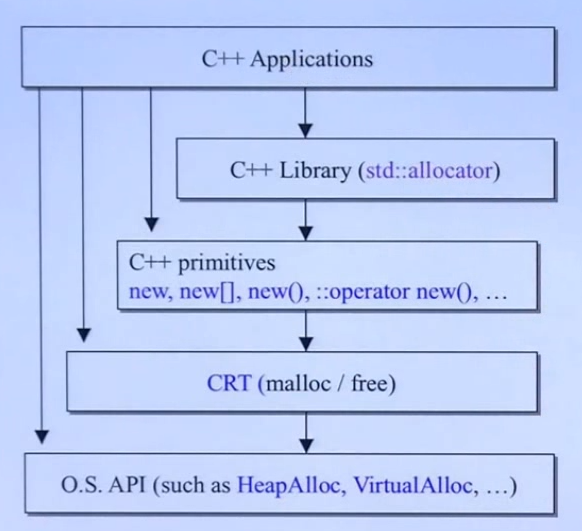
\includegraphics[scale = 0.5]{MemProcess.png}
				\caption{Mem Process}
			\end{figure}

		
		\subsection{内存管理基础要素}
			\begin{table}[H]
				\caption{C++ Memory Primitives}
				\begin{tabular}{llll}
					\toprule[1.5pt]
					分配& 释放& 类型& 可否重载\\
					\midrule[1pt]
					\verb|malloc()|&\verb|free()|& C 函数& 不可\\
					\verb|new|&		\verb|delete|& C++ 表达式& 不可\\
					\verb|::operator new()|& \verb|::operator delete()|& C++ 函数& 可\\
					\verb|allocator<T>::allocate()|& \verb|allocator<T>::deallocate()|& C++ 标准库& 可自由设计\\
					\bottomrule[1.5pt]
				\end{tabular}
			\end{table}	
			
			\newpage
			\paragraph{new}\verb|->|
				\begin{lstlisting}
	Complex* pc = new Complex(1,2);
	|
	|_____
		 |
		Complex* pc;
		try{
			void* mem = operator new( sizeof(Complex) ); // 1申请内存
			pc = static_cast<Complex*>(mem); // 2转型
			pc ->Complex::Complex(1,2);// 3调用构造函数
		} 
		catch(std::bad_alloc)
		{
			....
		}
				\end{lstlisting}
		
			
			\paragraph{operator new()}\verb|->|
				\begin{lstlisting}
	void* operator new(size_t size, const std::nothrow_t &)_THROW0()
	{
		void *p;
		while((p = malloc(size)) == 0)
		{
			_TRY_BEGIN
				if(_callnewh(size) == 0) break; // new handle: 当无内存使用用户指定处理函数进行处理
			_CATCH(std::bad_alloc) return (0);
			_CATCH_END
		}
		return (p);
	}
				\end{lstlisting}
		
			\paragraph{new(已分配内存指针 p) expression} \verb|placement new ->|
			
				给已分配内存调用合理的构造函数进行初始化。
				 
				\begin{lstlisting}
	new(p) Complex(1,2);				
				\end{lstlisting}
				
			\newpage
			\paragraph{array new, array delete}\verb|->|
				\begin{lstlisting}
	Complex* pca = new Complex[3];// 唤起3次 constructor, 无法从参数获取初值
	
	delete[] pca; //唤起3次deconstructor, 如果没有写中括号,那么会以为为普通指针,只调用一次析构。
				\end{lstlisting}
				
				\begin{figure}[H]
					\centering
					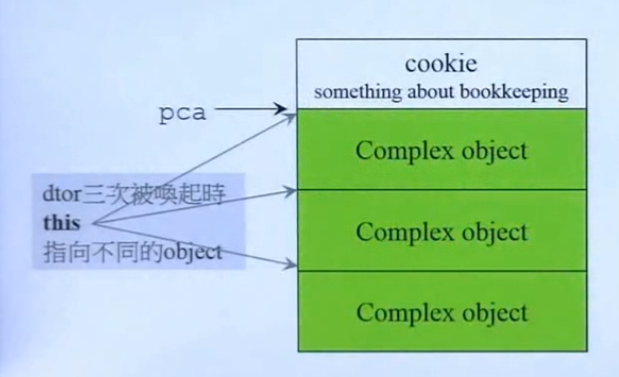
\includegraphics[scale = 0.5]{arrayNew.png}
					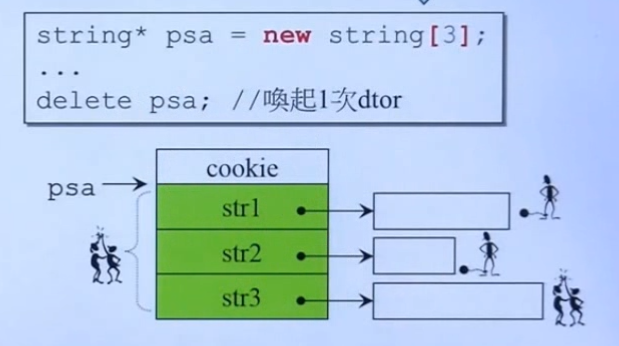
\includegraphics[scale = 0.5]{opArrayNew.png}
					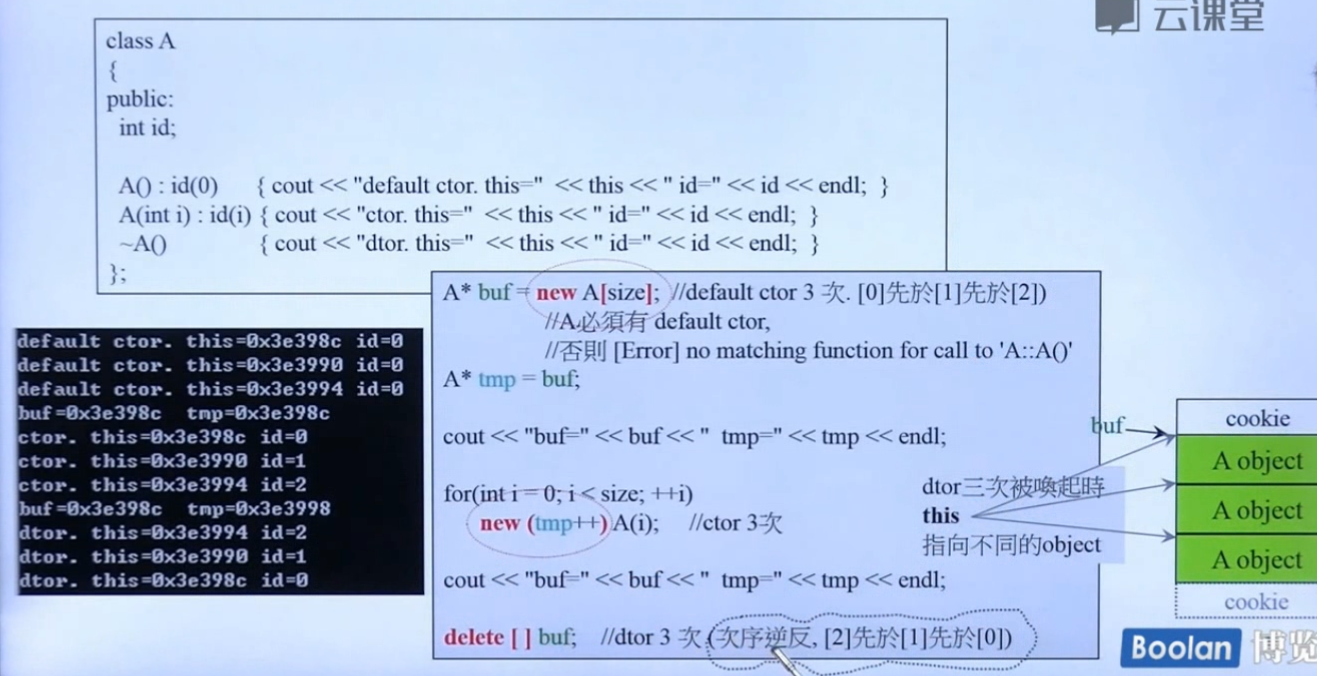
\includegraphics[scale = 0.3]{arrayNewExample.png}
					\caption{Array New Mem}
				\end{figure}
				
			\verb|cookie -> 负责记录申请数组的长度,即调用delete 的次数|		
			
			\newpage		
			\paragraph{delete}\verb|->|
				\begin{lstlisting}
	Complex* pc = new Complex(1,2);
		...
	delete pc;
	|
	|____
		 |
		 pc->~Complex(); // 先析构
		 operator delete(pc); // 然后释放内存
				\end{lstlisting}
	
			\paragraph{operator delete(void *)}\verb|->|
				\begin{lstlisting}
	void _cdecl operator delete(void*p) _THROW0()
	{
		free(p);
	}
				\end{lstlisting}
		
			\paragraph{总结-流程}示例\verb|->|
				\begin{lstlisting}
	Foo* p = new Foo(x);
		...
	delete p;
				\end{lstlisting}
	
				上述代码可具体表示为如下几个相关部分
				\begin{enumerate}[itemindent = 1em]
					\item \textbf{operator new :}\verb|Foo* p = (Foo*)operator new(sizeof(Foo));|
					
						notice: \verb|operator new -> Foo::operator new(size_t size)|即这里调用的是该类重载后的\verb|operator new|,如果没有发生重载则调用原\verb|operator new|,\verb|operator delete| 相同。
						
					\item \textbf{placement new :}\verb|new(p) Foo(x);|
					\item \textbf{deConstruct :}\verb|p->~Foo();|
					\item \textbf{operator delete :}\verb|operator delete(p);|
				\end{enumerate}
			
			\newpage	
			\paragraph{allocator}
				将内存管理的细节隔离实现,简化不同类的编写效率与安全性。
				
				\begin{lstlisting}
	class allocator
	{
	private:
		struct obj{
			struct obj* next; //embedded pointer
		}
	
	public:
		void *allocate(size_t);
		void deallocate(void*, size_t);
	
	private:
		obj* freeStore = nullptr;
		const int CHUNK = 5;
	};			
	
	void allocator::deallocate(void* p, size_t)
	{
		//将*p 收回插回freeList 前端
		((obj*)p) ->next = freeStore;
		freeStore =(obj*)p;
	}					
	
	
	// 什么类型的类都是如下使用allocator 的,因此会产生宏简化过程。
	class Foo{
	public:
		long L;
		string str;
		static allocator myAlloc;
		
	public:
		Foo(long l):L(l){}
		static void* operator new(size_t size)
		{
			return myAlloc.allocate(size);
		}
		
		static void operator delete(void* pdead, size_t size)
		{
			return myAlloc.deallocate(pdead,size);
		}
	
	};
	allocate Foo::myAlloc;
				\end{lstlisting}
			
			\newpage
			\paragraph{marco for static allocator}
				简化上述allcator 注入的代码量与程序员的工作量。
					
				\begin{lstlisting}
	// Declare pool alloc
	#define DECLARE_POOL_ALLOC()\
	public:\
		void* operator new(size_t size){return myAlloc.allocate(size);}\
		void operator delete(void* p){return myAlloc.deallocate(p);}\
	protected:\
		static allocator myAlloc;
	
	// Implement pool alloc
	#define IMPLEMENT_POOL_ALLOC(class_name)\
	allocator class_name::myAlloc;
	
	
	// class Foo 实现
	class Foo{
		DECLARE_POOL_ALLOC()
	public:
		long L;
		string str;
	public:
		Foo(long l):L(l){}
	};
	IMPLEMENT_POOL_ALLOC(Foo)
	
	class Goo{
	DECLARE_POOL_ALLOC()
	public:
		complex<double> c;
		string str;
	public:
			Foo(complex<double>& x):c(x){}
	};
	IMPLEMENT_POOL_ALLOC(Goo)
				\end{lstlisting}
				
			\paragraph{new Handler}
				当内存分配失败的情况下使用newHandler 进行处理,以释放空间满足分配或者终止程序。
			
		\subsection{malloc 申请空间布局结构}
			 
			在使用malloc 分配的内存中存在着大量的空余空间,如cookie 信息等,基本结构如图\ref{mem}所示。
			\begin{figure}[H]
				\centering
				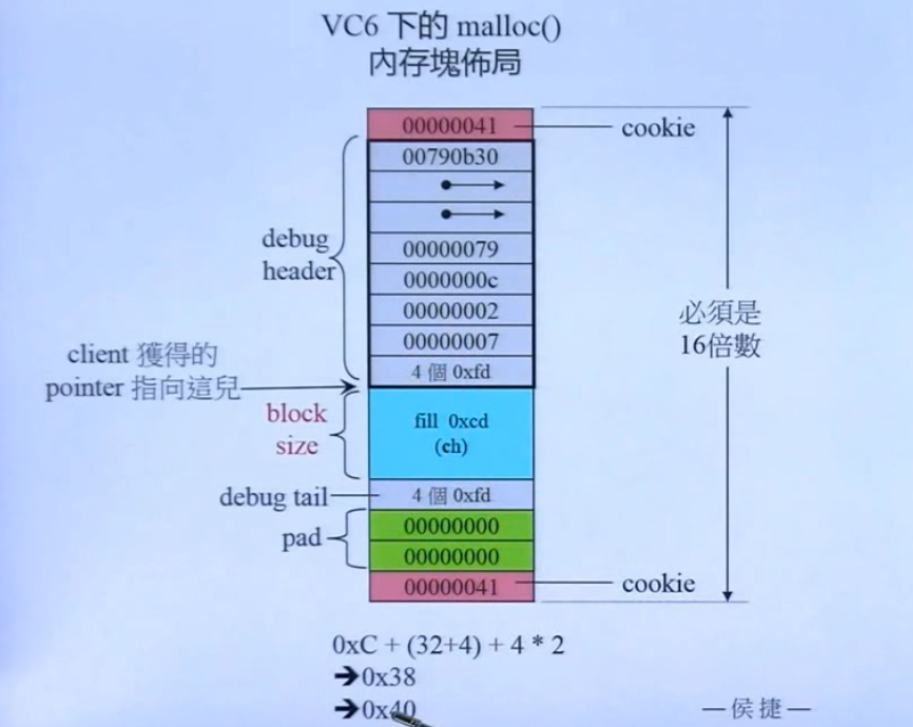
\includegraphics[scale = 0.5]{Malloc.png}
				\caption{Malloc 结构图}
				\label{mem}
			\end{figure}
	
		\subsection{embedded pointers}
			当客户端获得小区块,获得的即是char*(指向某个 union obj). 此时虽然客户端没有如LString 之类的信息可知区块大小,但由于这区块是给object 所用,相等于object 大小,object Constructor 自然不会过分。如图\ref{emb}所示。
			\begin{figure}[H]
				\centering
				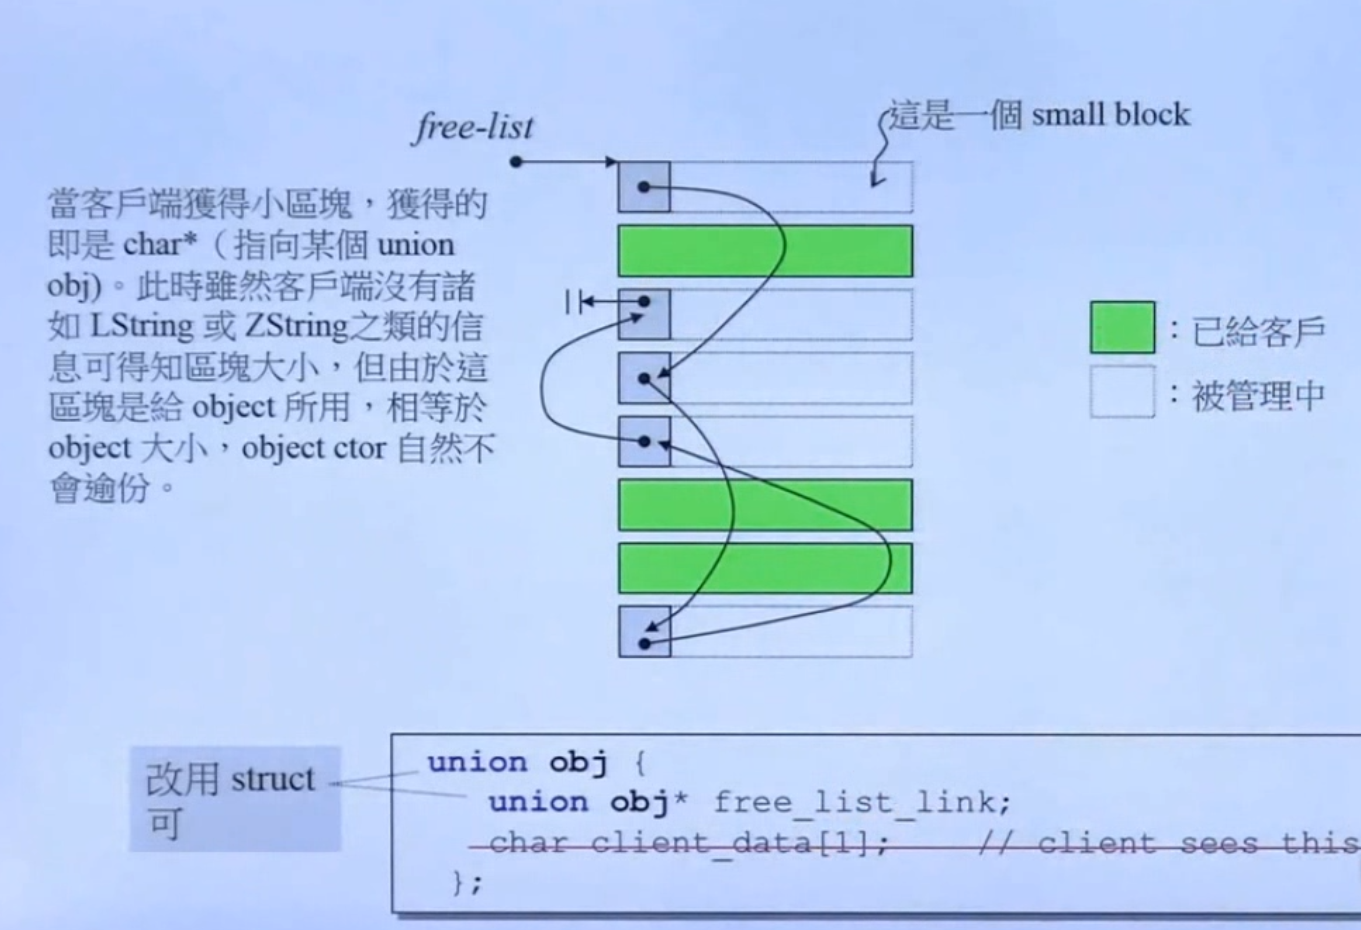
\includegraphics[scale = 0.3]{embeddedP.png}
				\caption{嵌入指针}
				\label{emb}
			\end{figure}
			
			\begin{lstlisting}
	class Airplane{
	private:
		// Data member 结构声明
		struct AirplaneRep{
			unsigned long miles;
			char type;
		};
		
	private:
		union{
			AirplaneRep rep;  // 此指针针对使用中的 objects
			Airplane* next;   //此指针针对内存池 freelist 上的object 
		}
	};
			\end{lstlisting}
	
	
	\section{STL 内存分配}
		\paragraph{STL freelist 何时释放}
			在看完源码后,知道了如何利用内存池进行管理内存,但是如果内存紧张,怎么知道freelist 何时释放呢?析构?引用计数?
			
		\paragraph{STL pool allocator用法示例}
			STL(GNUC 4.9)库中带有的内存池分配,但是标准的分配依旧是只调用new expression。
			
			\begin{lstlisting}
	#include <extend\pool_allocator.h>
	
	template<typename Alloc>
	void cookie_test(Alloc alloc, size_t n)
	{
		typename Alloc::value_type *p1, *p2, *p3;
		p1 = alloc.allocate(n);
		p2 = alloc.allocate(n);
		p3 = alloc.allocate(n);
		
		cout<<"p1 = " << p1 << '\t' <<"p2 = " << p2 <<'\t'<<endl;
		
		alloc.deallocate(p1, sizeof(typename Alloc::value_type));
		alloc.deallocate(p2, sizeof(typename Alloc::value_type));
		alloc.deallocate(p3, sizeof(typename Alloc::value_type));
	}
	
	
	// Test 主体
	int main()
	{
		// 使用标准内存池分配
		cout << sizeof(__gnu_cxx::__pool_alloc<int>) <<endl;
		vector<int, __gnu_cxx::__pool_alloc<int>> vecPool;
		cookie_test(__gnu_cxx::__pool_alloc<double>(), 1);
		
		// 使用默认分配器分配
		cout << sizeof(std::allocator<int>) <<endl;
		vector<int, std::allocator<int>> vecPool;
		cookie_test(std::allocator<double>(), 1);		
	}
			\end{lstlisting}
		
		
		\paragraph{原理概述}
			std::alloc \verb|->16 大小的链表| 负责分配(0-8-16-...-128bytes) 大小的内存管理池。超过128后,使用malloc 进行内存管理。
			
			战备
			
			如果x-size 的链表为空,且战备池已经占用,则申请20*(x-size)*2 的内存池,否则使用x-size 的对应指针指向该战备池,并在战备池中按照x-size 进行切割分配管理,*2的意图就是留相同的一份池用于战备,有则在内存池中分配。 
	
			\begin{figure}[H]
				\centering
				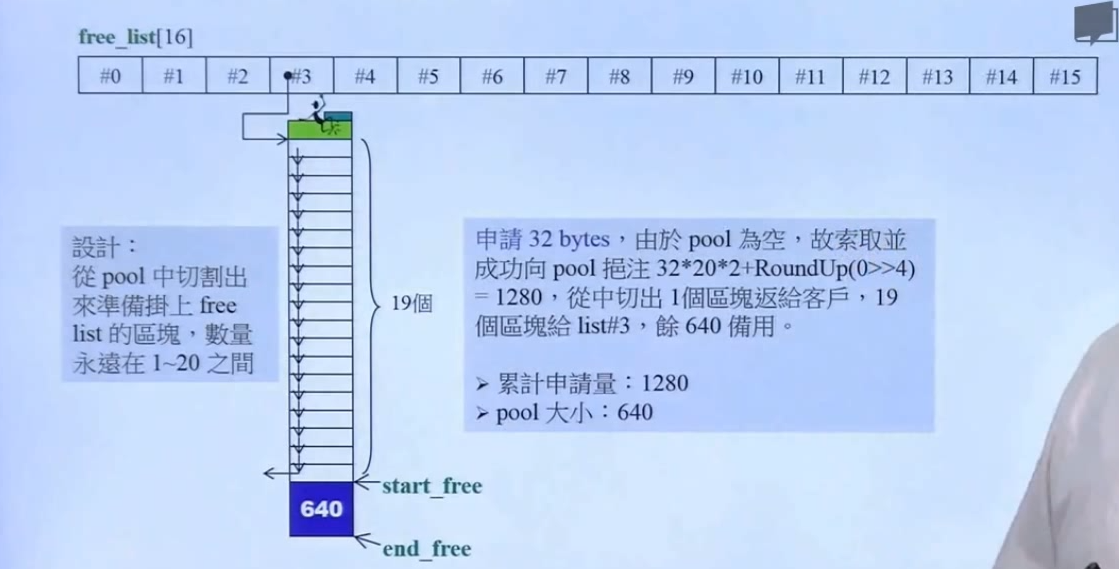
\includegraphics[scale=0.4]{STD_arc.png}
				\caption{STD alloctor 架构图}
			\end{figure}
			
		
			在可用空间为0时,\textbf{最多分配20个对象空间 }*2 +RoundUp。
		
			在剩余的战备空间不足一个对象时,就是\textbf{堆碎片的处理}。
		
		\paragraph{堆碎片处理}
			剩余的碎片插入最接近的链表中。
			
			\begin{figure}[H]
				\centering
				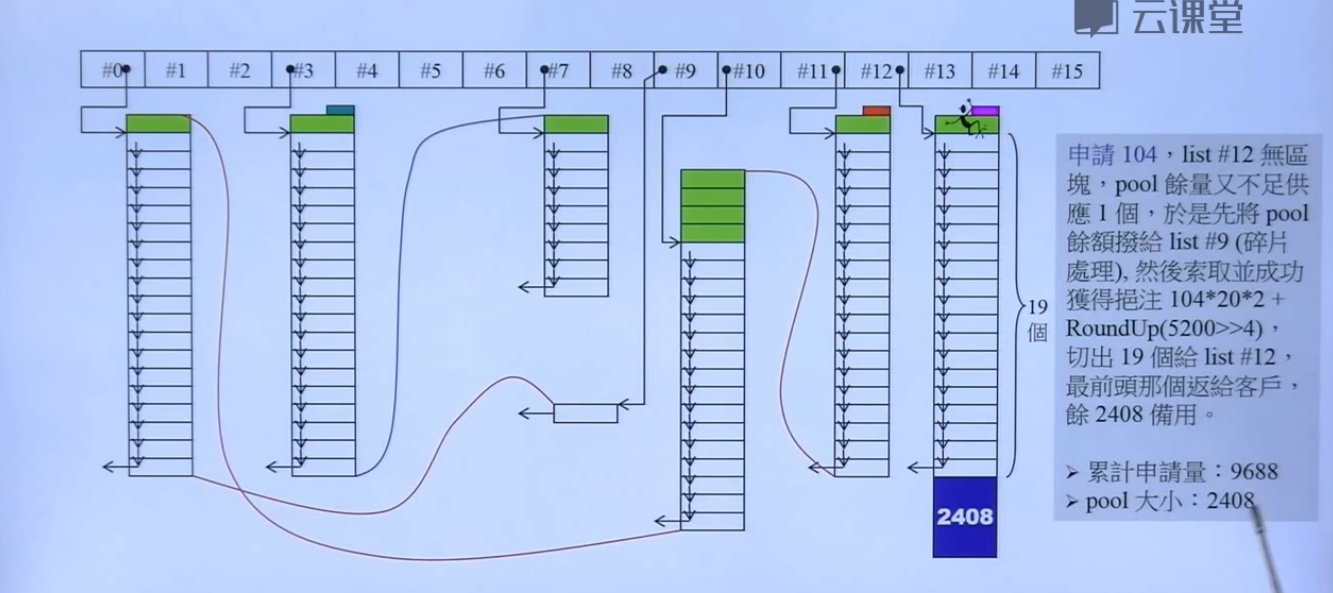
\includegraphics[scale=0.37]{headFragment.png}
				\caption{堆碎片处理流程}
			\end{figure}
		
		
		\paragraph{内存不足解决}
			依次往右借战备池满足当下需求
				

	\section{STL 源码结构}
		SGI的内存配置器分成两层:第一层直接调用malloc,第二层是自己做了一个内存池来分配。下面说下第二层配置器的思路:
		
		\verb|std::alloc|在\textbf{设计时}考虑到了以下几个方面:
			\begin{itemize}
				\item 向系统堆申请空间。
				\item 考虑多线程状态。
				\item 考虑内存不足时的措施。
				\item 考虑过多“小型区块”可能造成的内存碎片问题。
			\end{itemize}
		
		\textbf{二级配置器内存申请过程}:
			\begin{itemize}
				\item 首先判断是否小于128bytes。
				\item 若小于则把申请长度填充至8的倍数。
				\item 利用\verb|free_list+FREELIST_INDEX(n)|获取所需内存块在\verb|free-lists|链表中的位置。
				\item 若申请失败则调用\verb|refill给free-list|扩容。
				\item 若申请成功则将\verb|free-list|的头节点保存之后指向下一个节点,返回保存的地址。
			\end{itemize}
			
		第二层配置器首先设置了一个\verb|free_list[16]|的数组,数组中是指针,分别指向一块内存,指针类型定义如下:
		
		\begin{lstlisting}
	union obj {
	  union obj *free_list_link;
	  char client_data[1];
	};
		\end{lstlisting}
		
		总之,\verb|free_list|每个下标链接的内存大小为:8B、16B、24B、32B、40B、...、128B。共16个。
		
		现在假如要分配一块32B的内存,但\verb|free_list|[3]所指向的指针为NULL,即空闲链表\verb|free_list|中没有32B的内存,这时候就需要通过下面的\verb|_S_chunk_alloc|来分配内存给\verb|free_list|了。默认每次分配是分配20个大小为32B的内存。
		
		即\verb|_S_chunk_alloc|第二个参数传入值为20,但系统不一定能分配20个,所以用的是引用。\verb|_S_chunk_malloc|主要\textbf{分三种情况来处理}:
			\begin{itemize}
				\item 现有内存池容量满足你的需求:32B * 20个,直接返回给你这么大一块内存;
				\item 现有内存池容量不能满足这么多个,即20个,但可以满足1个,那先给你\verb|free_list|对应项分配一个32B再说;
				\item 现有内存池容量连一个都满足不了,那只能利用malloc从堆中分配内存。
			\end{itemize}
		
		从堆中分配内存时,首先把当前内存池中剩余的一些零碎内存赋给\verb|free_list|中;
		
		然后从堆中malloc内存,修改内存池的\verb|_S_start_free、_S_end_free|指针。(这两个指针分别指向内存池的起始地址和结束地址)。
		
		再然后递归调用\verb|_S_chunk_malloc|函数。
		  
		\paragraph{class allocator}\verb|class __default_alloc_template|

		\paragraph{allocate()}\verb|~|
			\begin{lstlisting}[frame = lines]
	static void* allocate(size_t __n)  
	{  
	    void* __ret = 0;  
	        
	    if (__n > (size_t) _MAX_BYTES)   
	        // 如果请求大于128字节,由一级内存配置器分配内存  
	    	__ret = __mem_interface::allocate(__n);  
	    else   
	    // 当内存请求小于等于128字节时  
	    {  
	           _Obj* volatile* __my_free_list = _S_free_list   
	             + _S_freelist_index(__n);  
	      //定位监管的freelist  
	  
	          _Obj* __restrict__ __result = *__my_free_list;  
	          if (__result == 0)  
	          //如果freelist是空的,则通过调用s_refill分配freelist  
	        __ret = _S_refill(_S_round_up(__n));  
	      else   
	          //如果freelist有空闲内存块,则返回一个空闲块给客户  
	          //同时监管freelist的头指针后移一个空闲块  
	          {  
	              *__my_free_list = __result -> _M_free_list_link;  
	              __ret = __result;  
	          }  
	      }  
	      return __ret;  
	};  
			\end{lstlisting}

		\paragraph{refill()}
			函数原型:\fbox{void* \_\_default\_alloc\_template::refill(size\_t n)}
			
			若free-list中没有可用区块时,则会调用refill为free-list填充新的空间。新的空间来自内存池,由chunk\_alloc()申请。默认是取得20个新区块,但是如果内存池空间不足,则获得的区块数可能小于20。如果chunk\_alloc()返回一个区块,则直接返回,将该区块分配给调用者使用。free-list不增加。若返回区块数大于1,则从第二个区块开始扩展free-list链表,每个链表占n的长度。将第一个区块返回。
			
			\begin{lstlisting}[frame = lines]
	 // Returns an object of size __n, and optionally adds to "size  
	 // __n"'s free list.  We assume that __n is properly aligned.  We  
	 // hold the allocation lock.  
	   
	template<bool __threads, int __inst>  
	   void*  
	   __default_alloc_template<__threads, __inst>::_S_refill(size_t __n)  
	  {  
	     int __nobjs = 20;   
	     //默认20个,实际client需求的20倍  
	     char* __chunk = _S_chunk_alloc(__n, __nobjs);  
	     //请求memory pool分配内存块,实际需求的20倍  
	     _Obj* volatile* __my_free_list;  
	     _Obj* __result;  
	     _Obj* __current_obj;  
	     _Obj* __next_obj;  
	     int __i;  
	       
	    if (1 == __nobjs) return(__chunk);  
	     
	    __my_free_list = _S_free_list + _S_freelist_index(__n);  
	       
	    __result = (_Obj*)__chunk;   
	    //将返回给客户20块内存区块的第一块地址  
	   *__my_free_list = __next_obj = (_Obj*)(__chunk + __n);  
	    //修改监管freelist的首地址为第一个空闲内存块的地址  
	  
	   for (__i = 1; ; __i++) {  
	       __current_obj = __next_obj;  
	       __next_obj = (_Obj*)((char*)__next_obj + __n);  
	       if (__nobjs - 1 == __i) {  
	         __current_obj -> _M_free_list_link = 0;  
	         break;  
	       } else {  
	         __current_obj -> _M_free_list_link = __next_obj;  
	       }  
	   }  
	  
	   //上述for循环,是将freelist中的各结点串接起来。  
	  
	    return(__result);  
	}  
			\end{lstlisting}
					
		\paragraph{chunk\_alloc()}
			函数原型:\fbox{char*  \_\_default\_alloc\_template::chunk\_alloc(size\_t size,int\& nobjs)}
			
			其中nobjs是引用传参,是传入传出参数。表示的是chunk申请到的区块数,默认是20。
			
			函数先判断内存池中剩余的空间是否满足申请20个内存区块,若满足则直接返回。若不满足,则尽量申请多的区块,并利用nobjs的返回值标明申请的区块数量。若内存池剩余的空间不够申请1个内存区块,则先将这剩余的区块分配给适当的free-list,然后再从系统堆中申请需求量的两倍加上附加量的内存空间,递归调用自己返回正确的nobjs值,由于nobjs最大为20,剩余的未加入free-list的内存放入内存池中。若从堆中申请失败,则遍历整个free-lists,看能否找到一个满足长度要求的内存区块。如果还是找不到,则调用一级配置器,也就是malloc(),利用它的异常机制来处理,若未定义处理函数,则抛出bad\_alloc异常。
			
			\begin{lstlisting}[frame = lines]
	template <bool __threads, int __inst>
	char*
	__default_alloc_template<__threads, __inst>::_S_chunk_alloc(size_t __size,
	                                                            int& __nobjs)
	{
	    char* __result;
	    size_t __total_bytes = __size * __nobjs;
	    size_t __bytes_left = _S_end_free - _S_start_free; // 内存池剩余空间
	 
	    if (__bytes_left >= __total_bytes) { // 内存池剩余空间完全满足需求
	        __result = _S_start_free;
	        _S_start_free += __total_bytes;
	        return(__result);
	    } else if (__bytes_left >= __size) { // 内存池剩余空间不能完全满足需求,但足够供应一个(含)以上的区块
	        __nobjs = (int)(__bytes_left/__size);
	        __total_bytes = __size * __nobjs;
	        __result = _S_start_free;
	        _S_start_free += __total_bytes;
	        return(__result);
	    } else { // 内存池剩余空间连一个区块的大小都无法提供
	        size_t __bytes_to_get =
	      2 * __total_bytes + _S_round_up(_S_heap_size >> 4);
	        // Try to make use of the left-over piece.
	        // 把内存池当前剩下的一些小残余零头利用一下。
	        if (__bytes_left > 0) {
	            _Obj* __STL_VOLATILE* __my_free_list =
	                        _S_free_list + _S_freelist_index(__bytes_left); // 这里对吗?假如__bytes_left = 15,则_S_freelist_index(15) = 1,
	                                                                        // 即16B的位置,而实际上只剩下了15B?
	 
	            ((_Obj*)_S_start_free) -> _M_free_list_link = *__my_free_list;
	            *__my_free_list = (_Obj*)_S_start_free;
	        }
	        _S_start_free = (char*)malloc(__bytes_to_get);
	        if (0 == _S_start_free) {
	            size_t __i;
	            _Obj* __STL_VOLATILE* __my_free_list;
	        _Obj* __p;
	            // Try to make do with what we have.  That can't
	            // hurt.  We do not try smaller requests, since that tends
	            // to result in disaster on multi-process machines.
	            for (__i = __size;
	                 __i <= (size_t) _MAX_BYTES;
	                 __i += (size_t) _ALIGN) {
	                __my_free_list = _S_free_list + _S_freelist_index(__i);
	                __p = *__my_free_list;
	                if (0 != __p) {
	                    *__my_free_list = __p -> _M_free_list_link;
	                    _S_start_free = (char*)__p;
	                    _S_end_free = _S_start_free + __i; // 这里确定每一块内存大小都是__i吗?
	                    return(_S_chunk_alloc(__size, __nobjs));
	                    // Any leftover piece will eventually make it to the
	                    // right free list.
	                }
	            }
	        _S_end_free = 0;    // In case of exception.
	            _S_start_free = (char*)malloc_alloc::allocate(__bytes_to_get);
	            // This should either throw an
	            // exception or remedy the situation.  Thus we assume it
	            // succeeded.
	        }
	        _S_heap_size += __bytes_to_get;
	        _S_end_free = _S_start_free + __bytes_to_get;
	        return(_S_chunk_alloc(__size, __nobjs));
	    }
	}
			\end{lstlisting}
			
			  可以看到\verb|chunk_alloc|函数的\textbf{输入}有两个:
			  	\begin{enumerate}
			  		\item \verb|int&__nobjs|,待分配的元素个数;
			  		\item \verb|size_t __size|,每个元素的大小。
			  	\end{enumerate}
			  
			\verb|chunk_alloc|函数的程序流程图(为了方便观察,画的并不是标准的程序流程图)如下:
				\begin{figure}[H]
					\centering
					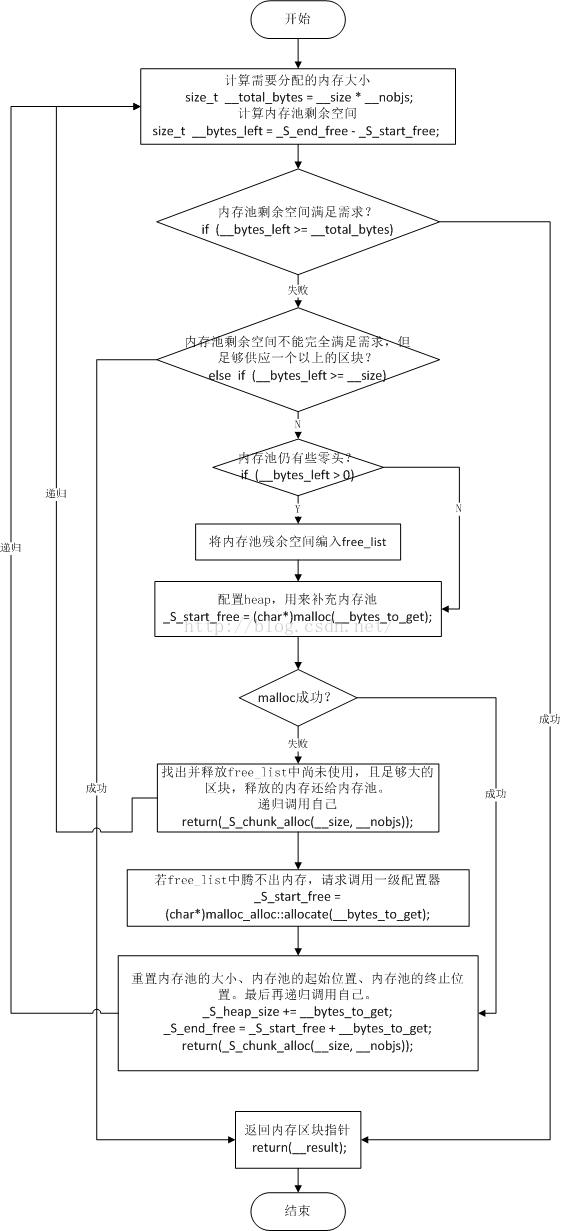
\includegraphics[scale=0.5]{chunk.png}
					\caption{chunkAlloc 流程}
				\end{figure}
				
		\paragraph{deallocate()}
			若回收长度大于128bytes则直接调用一级配置器,也就是::operator delete。否则就在free-lists上寻找对应大小的区块,调整该free-list,回收区块。
				
			\begin{lstlisting}[frame = lines]
	static void   
	    deallocate(void* __p, size_t __n)  
	    {  
	      if (__n > (size_t) _MAX_BYTES)  
	    __mem_interface::deallocate(__p, __n);  
	      else   
	      {  
	      _Obj* volatile*  __my_free_list  
	        = _S_free_list + _S_freelist_index(__n);  
	      _Obj* __q = (_Obj*)__p;  
	        
	      __q -> _M_free_list_link = *__my_free_list;  
	      *__my_free_list = __q;  
	     }  
	    }  
			\end{lstlisting}
					
	\section{内存泄漏}
		\subsection{如何对付内存泄漏?}
			当你的代码中到处充满了new 操作、delete操作和指针运算的话,你将会在某个地方搞晕了头,导致内存泄漏,指针引用错误,以及诸如此类的问题。
			这和你如何小心地对待内存分配工作其实完全没有关系:代码的复杂性最终总是会超过你能够付出的时间和努力。于是随后产生了一些成功的技巧,它们依赖于\textbf{将内存分配(allocations)与重新分配(deallocation)工作隐藏在易于管理的类型之后}。
			
			标准容器(standard containers)是一个优秀的例子。它们不是通过你而是自己为元素管理内存,从而避免了产生糟糕的结果。
			
			\textbf{模板和标准库}实现了\textit{容器、资源句柄以及诸如此类的东西},更早的使用甚至在多年以前。异常的使用使之更加完善。
			
			如果你实在不能将内存分配/重新分配的操作隐藏到你需要的对象中时,你可以使用资源句柄(resource handle),以将内存泄漏的可能性降至最低。这里有个例子:我需要通过一个函数,在空闲内存中建立一个对象并返回它。这时候可能忘记释放这个对象。毕竟,我们不能说,仅仅关注当这个指针要被释放的时候,谁将负责去做。使用资源句柄,这里用了标准库中的\verb|auto_ptr|,使需要为之负责的地方变得明确了。
			
		\subsection{内存泄漏的发生方式}
			\begin{itemize}
				\item 常发性内存泄漏。
				\item 偶发性内存泄漏。
				\item 一次性内存泄漏。
				\item \textbf{隐式内存泄漏}。程序在运行过程中\textit{不停的分配内存,但是直到结束的时候才释放内存}。严格的说这里并没有发生内存泄漏,因为最终程序释放了所有申请的内存。但是对于一个服务器程序,需要运行几天,几周甚至几个月,\textbf{不及时释放内存也可能导致最终耗尽系统的所有内存。}所以,我们称这类内存泄漏为隐式内存泄漏。举一个例子:
				\begin{lstlisting}
	class Connection
	{
		public:
		Connection( SOCKET s);
		~Connection();	
		…	
		private:
		SOCKET _socket;
		…	
	};
	
	class ConnectionManager	
	{
		public:
		ConnectionManager(){}
		
		~ConnectionManager(){
			list::iterator it;
			
			for( it = _connlist.begin(); it != _connlist.end(); ++it ){
				delete (*it);
			}
			_connlist.clear();
		}
		
		void OnClientConnected( SOCKET s ){
			Connection* p = new Connection(s);
			_connlist.push_back(p);
		}
		
		void OnClientDisconnected( Connection* pconn ){
			_connlist.remove( pconn );
			delete pconn;	
		}
		private:
		list _connlist;	
	};
				\end{lstlisting}
				假设在Client从Server端断开后,Server并没有呼叫OnClientDisconnected()函数,那么代表那次连接的Connection对象就不会被及时的删除(在Server程序退出的时候,所有Connection对象会在ConnectionManager的析构函数里被删除)。当不断的有连接建立、断开时隐式内存泄漏就发生了。
				
				从用户使用程序的角度来看,内存泄漏本身不会产生什么危害,作为一般的用户,根本感觉不到内存泄漏的存在。真正有危害的是\textbf{内存泄漏的堆积},这会最终消耗尽系统所有的内存。从这个角度来说,一次性内存泄漏并没有什么危害,因为它不会堆积,\textbf{而隐式内存泄漏危害性则非常大,因为较之于常发性和偶发性内存泄漏它更难被检测到。}
				
			\end{itemize}
		\subsection{C/C++内存泄漏及其检测工具}
			
			
			
		\subsection{检测内存泄漏}
			
			
			
	\section{内存回收}
		C++将内存划分为\textbf{三个逻辑区域}:\textit{堆、栈和静态存储区}。既然如此,我称位于它们之中的对象分别为堆对象,栈对象以及静态对象。那么这些不同的内存对象有什么区别了?堆对象和栈对象各有什么优劣了?如何禁止创建堆对象或栈对象了?
		
		\subsection{内存对象大会战}
			\textbf{几乎所有的临时对象都是栈对象}。比如,下面的函数定义:
			
			\verb|Type fun(Type object);|
			
			这个函数至少产生两个临时对象,首先,参数是按值传递的,所以会调用拷贝构造函数生成一个临时对象\verb|object_copy1| ,在函数内部使用的不是使用的不是object,而是\verb|object_copy1|,自然,\verb|object_copy1|是一个栈对象,它在函数返回时被释放;还有这个函数是值返回的,在函数返回时,如果我们不考虑返回值优化(NRV),那么也会产生一个临时对象\verb|object_copy2|,这个临时对象会在函数返回后一段时间内被释放。
			
			\textbf{静态存储区}。所有的\textit{静态对象、全局对象都于静态存储区分配}。关于全局对象,是在\textbf{main()函数执行前}就\textit{分配好了的}。其实,在main()函数中的显示代码执行之前,会调用一个由编译器生成的\verb|_main()|函数,而\verb|_main()|函数\textbf{会进行所有全局对象的的构造及初始化工作}。而\textit{在main()函数结束之前},\textbf{会调用由编译器生成的exit函数,来释放所有的全局对象}。
			
			那么,\textbf{局部静态对象}了?局部静态对象通常也是在函数中定义的,就像栈对象一样,只不过,其前面多了个static关键字。\textbf{局部静态对象的生命期}是从其所在函数第一次被调用,更确切地说,\textit{是当第一次执行到该静态对象的声明代码时,产生该静态局部对象,直到整个程序结束时,才销毁该对象。}
			
			\textbf{class的静态成员}?class的\textbf{静态成员对象的生命期},class的静态成员对象\textit{随着第一个class object的产生而产生,在整个程序结束时消亡。}也就是有这样的情况存在,在程序中我们定义了一个class,该类中有一个静态对象作为成员,但是在程序执行过程中,\textit{如果我们没有创建任何一个该class object,那么也就不会产生该class所包含的那个静态对象}。还有,\textit{如果创建了多个class object,那么所有这些object都共享那个静态对象成员}。
			
			
			
		\subsection{垃圾回收方法}
			许多 C 或者 C++ 程序员对垃圾回收嗤之以鼻,认为垃圾回收肯定比自己来管理动态内存要低效,而且在回收的时候一定会让程序停顿在那里,而如果自己控制内存管理的话,分配和释放时间都是稳定的,不会导致程序停顿。最后,很多 C/C++ 程序员坚信在C/C++ 中无法实现垃圾回收机制。这些错误的观点都是由于不了解垃圾回收的算法而臆想出来的。
			
			\textbf{其实垃圾回收机制并不慢,甚至比动态内存分配更高效。}因为我们可以只分配不释放,那么分配内存的时候只需要从堆上一直的获得新的内存,移动堆顶的指针就够了;而释放的过程被省略了,自然也加快了速度。现代的垃圾回收算法已经发展了很多,增量收集算法已经可以让垃圾回收过程分段进行,避免打断程序的运行了。而传统的动态内存管理的算法同样有在适当的时间收集内存碎片的工作要做,并不比垃圾回收更有优势。
			
			而\textbf{垃圾回收的算法}的\textbf{基础}通常\textit{基于扫描并标记当前可能被使用的所有内存块},\textit{从已经被分配的所有内存中把未标记的内存回收来做的}。C/C++ 中无法实现垃圾回收的观点通常基于无法正确扫描出所有可能还会被使用的内存块,但是,看似不可能的事情实际上实现起来却并不复杂。
			
			首先,通过扫描内存的数据,指向堆上动态分配出来内存的指针是很容易被识别出来的,如果有识别错误,也只能是把一些不是指针的数据当成指针,而不会把指针当成非指针数据。这样,回收垃圾的过程只会漏回收掉而不会错误的把不应该回收的内存清理。
			
			其次,如果回溯所有内存块被引用的根,只可能存在于全局变量和当前的栈内,而全局变量(包括函数内的静态变量)都是集中存在于 bss 段或 data段中。
			
			垃圾回收的时候,只需要扫描 bss 段, data 段以及当前被使用着的栈空间,找到可能是动态内存指针的量,把引用到的内存递归扫描就可以得到当前正在使用的所有动态内存了。
			
			如果肯为你的工程实现一个不错的垃圾回收器,提高内存管理的速度,甚至减少总的内存消耗都是可能的。如果有兴趣的话,可以搜索一下网上已有的关于垃圾回收的论文和实现了的库,\textbf{开拓视野对一个程序员尤为重要}。
	
\chapter{装载链接原理}
	参考文献:\url{https://tech.meituan.com/linker.html}
	
	为了让读者可以对源代码如何编译到二进制可执行程序有一个整体的了解,将会从一下几个方面介绍一下程序编译,链接和装载的基本原理。
	
	\section{CPU体系}
		我们现在大部分同学接触到的 PC 机或者服务器使用的 CPU 都是 \verb|X86_64| 指令集体系结构,这是一种基于 CISC(复杂指令集体系结构)。我们在计算机组成原理的课程里面都学到,其实CPU指令集类型中除了 CISC,还有另外一种 RISC 类型的 CPU 体系结构,也就是简单指令集体系结构,比如 SUN 的 SPARC 指令集,IBM 的 PowerPC 指令集都是基于 RISC 指令集的 CPU 体系结构。我们这里不去深究各种体系结构的细节,我们关心的是\textbf{在其中一种 CPU 体系结构中编译的代码能够在另一种体系结构下面运行么?}
		
		答案是否定的,因为所谓的二进制程序,其实都是有一条一条的 CPU 指令组成,二进制程序执行的过程中,也是由 CPU 把这些指令 load 到指令流中一条一条执行。不同的 CPU 体系结构的指令集是不一样的,指令的长度和组成都有区别。\textbf{所以让SPARC的CPU去执行一个编译成 X86 的 CPU 指令集的二进制程序是不可行的}。
	
	
	\section{跨平台原理}
		为什么经过 \verb|gcc/g++| 编译过的二进制程序不能跨平台执行呢?
		
		\verb|java| 程序能够跨平台执行是因为不同系统平台上面安装的 \verb|java 虚拟机|能够识别同一种 \verb|java 字节码|。
		那么我们是不是可以推断,不同的操作系统二进制程序不能跨平台执行,\textbf{是因为不同操作系统下面二进制文件的格式不同}呢?
		
		事实确实是这样的。我们都知道的是一个程序编译成二进制之后,运行的时候是\verb|从 main 函数|开始执行的。但是这个\textbf{程序是怎么样 load 到内存中的},\textbf{执行流又是如何准确的定位到 main 函数的地址的}。其实这些工作都是操作系统替我们做的。
		
		首先,操作系统肯定要\textbf{分配一块虚拟地址空间};
		
		然后,系统需要把二进制程序中的\textbf{代码和数据 load 到这个地址空间中},
		
		随后,系统会\textbf{根据某种特定的文件格式},找到其中某一个特定的位置(初始化段),\textit{做一些程序运行前的初始化工作},比如环境变量初始化和全局变量的处理,然后开始执行我们的 main 函数。\textbf{这里的“某种特定的文件格式”就是为什么二进制程序不能跨平台运行的原因。}
		
		这里我真正想说的是,\textbf{每一种操作系统有自己的二进制文件格式},操作系统把二进制可执行程序load到内存中之后,会根据默认的这种格式寻找各种数据,比如代码段,数据段和初始化段。所以说 \verb|Windows| 下面的 \verb|exe 可执行文件|,lib 静态库,dll 动态库是不可以直接运行在 Linux 系统下面的;\verb|MacOS| 下面的 \verb|Mach-O 可执行文件|,静态链接库(a库),动态链接库(so库)也是不能够直接放在 Linux 系统下面运行的。反之亦然,\verb|Linux| 下面的 \verb|ELF 可执行文件|,静态链接库(a库),动态链接库(so库)同样不能够在 Window 系统下面运行。
	
	\section{C例子->编译器与链接器}
		说完了 CPU 体系结构和操作系统对二进制文件格式的影响,下面我们从几个例子看一下从源代码文件如何经过处理最终变成一个可执行文件。不同的系统下有不同的编译器,比如 Windows 下有 vs 自带的 C++ 编译器,Linux 和 Unix 下面有 gcc/g++ 编译器。也有很多不同的编程语言,各自有自己的编译器把相应的源代码编译成二进制可执行程序。尽管有些实现细节不同,这些编译器的工作原理和过程是一致的。由于 Linux 和 c语言使用相对广泛,同时笔者对 Linux 和C/C++相对熟悉,本文剩下的部分都是基于在 Linux 平台下使用 gcc/g++ 编译器编译 c/c++ 源代码进行说明和解释。
		
		本文的初衷是让工程师对程序源代码如何通过编译器,链接器和装载器最终成为一个进程运行在系统中的整个过程有一个基本的理解,所以并不会涉及到编译器如何通过进行词法分析,语法分析和语义分析最终得到目标二进制文件。因此本文剩下的部分主要集中在 gcc/g++ 如何形成一个 Linux 认识的 elf 可执行文件的。
	
			\subsection{C源文件}
				\begin{lstlisting}
	int g_a = 1;            //定义有初始值全局变量
	int g_b;                 //定义无初始值全局变量
	static int g_c;         //定义全局static变量
	extern int g_x;         //声明全局变量
	extern int sub();     //函数声明
	
	int sum(int m, int n) {        //函数定义
		return m+n;
	}
	int main(int argc, char* argv[]) {
		static int s_a = 0;     //局部static变量
		int l_a = 0;                 //局部非static变量
		sum(g_a,g_b);
		return 0;
	}
				\end{lstlisting}
			
			\subsection{目标文件}
			
				在我们用 gcc 编译这个程序来查看编译器做了哪些事情之前,其实我们可以简单梳理一下,为了让这个程序能够运行起来,编译器至少都需要做哪些事情。
				
				首先,我们都会默认 CPU 会根据程序的代码一条一条执行;其实,当遇到了条件判断或者函数调用,程序就会发生指令流的跳转;还有,程序代码执行的过程中需要操作各种变量指向的数据。从这三个“理所当然”的行为里面,我们可以推断出编译器至少需要做哪些事情。
				
				第一,CPU 肯定不能理解这些高级语言代码,\textbf{编译器需要把代码编译成二进制指令}。 
				
				第二,指令流跳转的时候,\textbf{CPU 怎么能找到要跳转的位置,编译器需要为每个定义的函数所在的位置定义一个标签,每个标签有一个地址,调用每个函数的时候就相当于跳转到那个标签指向的地址}。 
				
				第三,CPU 如何能找到那些变量指向的数据,\textbf{编译器需要为每一个变量定义一个标签,每个标签同样有一个地址,这个地址指向内存中的数据空间}。
			
				我们来实际看一下编译器的行为,我们先把这个这个编译成目标文件看一下:
				
				\verb|gcc -c test.c -o test.o && nm test.o|
				\begin{lstlisting}
	0000000000000000 D g_a
	0000000000000004 C g_b
	0000000000000000 b g_c
					 U g_x
	0000000000000014 T main
	0000000000000004 b s_a.1597
	0000000000000000 T sum
				\end{lstlisting}
				
				
				首先我们用 \verb|gcc -c 命令|把 \verb|test.c| 源码文件编译成 \verb|test.o| 目标文件,需要注意的是虽然目标文件也是二进制文件,但是和可执行文件是有区别的,目标文件仅仅把当前的源码文件编译成二进制文件,并没有经过链接过程,是不能够执行的。
				然后我们用 \verb|nm 命令|可以\textbf{查看一下目标文件的 symbol 信息}。这里我们看到了nm命令的输出默认有三列,其中\textbf{最左边}的一列是\textit{变量的相对地址},\textbf{中间的}一列表示变量所在的\textit{段的类型},\textbf{右面}表示\textit{变量的名字}。
				
				\begin{itemize}
					\item 首先最左边这一列是变量在所在\textbf{段的相对地址},我们看到\verb| g_a 和 g_c| 的相对地址是相同的,这并不冲突,因为他们处于不同的段中( D 和 b 表示它们在目标文件中处于不同的段中)。
					\item 第二列表示变量所处的\textbf{段的类型},比如我们这里看到了有 D,C,b,T 这些类型的段,实际上编译器支持的段类型比这个还多。我们同样不去深究各个段类型的意思,只要明白不同的段存放的是不同的数据即可,比如 \textbf{D 段就是数据段},专门\textit{存放有初始值的全局变量},\textbf{T 段表示代码段},所有的\textit{代码编译后的指令}都放到这个段中。在这里我们可以注意到同一个段中的变量\textit{相对地址是不能重复的}。
					\item 第三列表示变量的名字,这里我们看到局部的静态变量名字被编译器修改为 \verb|s_a.1597|,我们应该能猜得到编译器这么做的原因。\verb|s_a| 是一个\textit{局部静态变量},作用域限制在定义它的代码块中,所以我们可以在不同的作用域中声明相同名字的局部静态变量,比如我们可以在sum函数中声明另外一个 \verb|s_a|。但是我们上面提过,局部静态变量属于全局变量的范畴,它是存在于程序运行的整个生命周期的,所以为了支持这个功能,编译器对这种\textit{局部的静态变量名字加了一个后缀以便标识不同的局部静态变量}。
				\end{itemize}
				
				为什么这里的变量声明 \verb|g_x| \textbf{没有地址}呢?我们在C源码文件部分曾经提到过,\textbf{变量和函数的声明本质}上是\textit{给编译器一个承诺},告诉编译器虽然在本文件中没有这个变量或者函数定义,但是在其他文件中一定有,\textbf{所以当编译器发现程序需要读取这个变量对应的数据,但是在源文件中找不到的时候,就会把这个变量放在一个特殊的段(段类型为 U)里面,表示后续链接的时候需要在后面的目标文件或者链接库中找到这个变量,然后链接成为可执行二进制文件。}
				
				从上面这些信息的解释其实我们可以看出来,编译器没有那么复杂,它做的任何事情都是为了支持语言级别的功能。
				
			\subsection{目标文件的链接}
				上节我们留下了一个需要在其他目标文件中寻找的变量名。这一小节,我们讨论一下,在编译器把各个 C 源代码文件编译成目标文件之后,链接器需要对这些目标文件做什么样的处理。
				
				首先我们尝试一下对上一小节得到的目标文件链接一下看看有什么结果:\verb|gcc test.o -o test|
				\begin{lstlisting}
	test.o: In function `main':
	test.c:(.text+0x2c): undefined reference to `g_x'
	collect2: ld returned 1 exit status
				\end{lstlisting}
			
				当我们尝试把这个目标文件进行链接成为可执行文件时,链接器报错了。因为我们之前通过变量声明\textbf{承诺过的变量并没有在其他的目标文件或者库文件中找到},所以链接器无法得到一个完整可执行程序。我们尝试用另外一个 C 程序修复这个问题:
				\begin{lstlisting}
	int g_x = 100;
	int sub() {}
				\end{lstlisting}
				
				把这个文件编译成目标文件\verb|gcc -c test2.c -o test2.o; nm test2.o|
				\begin{lstlisting}
	0000000000000000 D g_x
	0000000000000000 T sub
				\end{lstlisting}
				
				现在我们尝试把这两个目标文件链接成为可执行文件:\verb|gcc test.o test2.o -o test; nm test|, 这时我们发现输出了比目标文件多很多的信息,其中定义了很多为了实现不同语言级别的功能而需要的段,在这里我们关心的是源文件中定义的那些变量对应的 symbol 及其地址,如下图所示:
				\begin{lstlisting}
	00000000004005e8 T _fini
	0000000000400390 T _init
	00000000004003d0 T _start
	...
	0000000000601018 D g_a
	0000000000601038 B g_b
	0000000000601030 b g_c
	000000000060101c D g_x
	00000000004004c8 T main
	0000000000601034 b s_a.1597
	0000000000400504 T sub
	00000000004004b4 T sum
				\end{lstlisting}
				
				在最终的可以执行文件里面,我们可以看到,首先,之前在第一个源文件中\verb|声明的变量g_x |和\verb|声明的函数 sub| 最终在第二个目标文件中\textbf{找到了定义};其次,在不同目标文件中定义的变量,比如 \verb|g_a、 g_x |都会放在了数据段中(段类型为 D);还有,\textbf{之前在目标文件中变量的相对地址全部变成了绝对地址}。
				
				所以我们再一次进行总结一下\textbf{链接器需要对源代码进行的处理}:
				\begin{itemize}[itemindent = 1em]
					\item 对各个目标文件中没有定义的变量,在其他目标文件中寻找到相关的定义。
					\item 把不同目标文件中生成的同类型的段进行合并。
					\item 对不同目标文件中的变量进行地址重定位。
				\end{itemize}
				
				这也是链接器所需要实现的最基本的功能。
				
	\section{执行期间->装载器程序}
		上面的几个小节中我们讨论了编译器把一个 C 源码文件编译成一个目标文件需要做的最基本的处理,也讨论了链接器把多个目标文件链接成可执行文件时需要具备的最基本的功能。在这一个小节我们来讨论一下可执行文件如何被系统装载运行的。
		
		\subsection{动态链接库}
			我们都知道,在我们写程序的过程中,不会自己实现所有的功能,一般情况下会调用我们所需要的系统库和第三方库来实现我们的功能。在上面两个小节的示例代码中,为了说明问题的简单起见,我们仅仅声明,定义了几个变量和函数,并没有使用任何的库函数。那么现在假设我们需要调用一个库函数提供的功能,这个时候可执行文件又是什么样的呢,我们再看一个小例子:
			
			\begin{lstlisting}
	#include <stdio.h>
	#include <string.h>
	
	int main(int argc, char* argv[]) {
		char buf[32];
		strncpy(buf, "Hello, World\n", 32);
		printf("%s",buf);
	}
			\end{lstlisting}
		
			我们把这个文件编译成可执行文件并且查看一下它的symbols:
			
			\verb|gcc test3.c -o test3; nm test3|
			\begin{lstlisting}
	00000000004005b4 T main
						U printf@@GLIBC_2.2.5
						U strncpy@@GLIBC_2.2.5		
			\end{lstlisting}
			
			现在我们检查的是可执行文件,为什么可执行文件里面仍然有这种没有地址的 symbols 呢?
			
			这里可执行文件中的“未定义”的 symbols 其实\textbf{是为了支持动态链接库的功能}。
			
			我们先来回顾一下动态链接库应该有一个什么样的功能。\textbf{所谓动态链接库是指,程序在运行的时候才去定位这个库,并且把这个库链接到进程的虚拟地址空间}。对于某一个动态链接库来说,所有使用这个库的可执行文件都共享同一块物理地址空间,这个物理地址空间在当前动态链接库第一次被链接时 load 到内存中。
			
			现在我们看一下二进制文件中对动态链接库中的函数怎么处理的,\verb@objdump -D test3 | less@,搜索\verb|printf|我们应该能看到以下内容:
			\begin{lstlisting}
	0000000000400490 <strncpy@plt>:
	400490:       ff 25 6a 0b 20 00       jmpq   *0x200b6a(%rip)        # 601000 <_GLOBAL_OFFSET_TABLE_+0x18>
	400496:       68 00 00 00 00          pushq  $0x0
	40049b:       e9 e0 ff ff ff          jmpq   400480 <_init+0x20>
	...
	00000000004004b0 <printf@plt>:
	4004b0:       ff 25 5a 0b 20 00       jmpq   *0x200b5a(%rip)        # 601010 <_GLOBAL_OFFSET_TABLE_+0x28>
	4004b6:       68 02 00 00 00          pushq  $0x2
	4004bb:       e9 c0 ff ff ff          jmpq   400480 <_init+0x20>
			\end{lstlisting}
			
			我们看到可执行文件中为 \verb|strncpy 和 printf| 分别生成了三个代理 symbol,然后代理 symbol 指向的第一条指令就是跳转到\verb|_GLOBAL_OFFSET_TABLE_|这个 symbol 对应的代码段中的一个偏移位置,而在 linux 中,这个\verb|_GLOBAL_OFFSET_TABLE_|对应的代码段是为了给\textbf{“地址无关代码”做动态地址重定位用的}。
			我们提过,\textbf{动态链接库可以映射到不同进程的不同的虚拟地址空间},所以属于“地址无关代码”,\textbf{链接器把对这个函数的调用代码跳转到程序运行时动态装载地址}。
			
			Linux 提供了一个很方便的命令查看一个可执行文件依赖的动态链接库,我们查看一下当前可执行文件的动态库依赖情况:\verb|ldd test3|:
			\begin{lstlisting}
    linux-vdso.so.1 =>  (0x00007fff413ff000)
    libc.so.6 => /lib/x86_64-linux-gnu/libc.so.6 (0x00007fe202ae7000)
    /lib64/ld-linux-x86-64.so.2 (0x00007fe202eb2000)	
			\end{lstlisting}
			
			\verb|ldd 命令|模拟\textbf{加载可执行程序需要的动态链接库,但并不执行程序},后面的地址部分表示模拟装载过程中动态链接库的地址。\textbf{如果尝试多次运行} \verb|ldd| 命令,我们会发现每次动态链接库的地址都是不一样的,\textbf{因为这个地址是动态定位的}。
			
			我们平常工作中,如果某一个二进制可执行文件报错找不到某个函数定义,可以用这个命令检查是否系统丢失或者没有安装某一个动态链接库。
			
			我们在上面的小程序最后加一个\verb|sleep(1000);|,然后查看一下运行时的内存映射分配,
			
			\verb|cd /proc/21509 && cat maps|,应该可以看到下面这一段:
			\begin{lstlisting}
	7feeef61f000-7feeef7d4000 r-xp 00000000 fd:01 135891                     /lib/x86_64-linux-gnu/libc-2.15.so
	7feeef7d4000-7feeef9d3000 ---p 001b5000 fd:01 135891                     /lib/x86_64-linux-gnu/libc-2.15.so
	7feeef9d3000-7feeef9d7000 r--p 001b4000 fd:01 135891                     /lib/x86_64-linux-gnu/libc-2.15.so
	7feeef9d7000-7feeef9d9000 rw-p 001b8000 fd:01 135891                     /lib/x86_64-linux-gnu/libc-2.15.so
			\end{lstlisting}
			
			我们可以看到进程运行时,系统为\verb| libc |库在进程地址空间中映射了四个段,因为每个段权限不同,所以不能合并为一个段。\textbf{对这些动态链接库的调用最终会跳转到这里显示的地址中。}
			
			根据以上这些信息,我们在这里继续总结一下\textbf{链接器需要对动态链接库需要做的最基本的事情}:
			\begin{itemize}[itemindent = 1em]
				\item 链接库在将目标文件链接成可执行文件的时候如果发现某一个变量或者函数在目标文件中找不到,会按照 \verb|gcc 预定义|的动态库寻找路径寻找动态库中定义的变量或者函数。
				\item 如果链接库在某一个动态链接库中找到了该变量或者函数定义,链接库首先会把这个动态链接库写到可执行文件的依赖库中,然后生成这个当前变量或者函数的代理 symbol。
				\item  在\verb|_GLOBAL_OFFSET_TABLE_|代码中生成真正的动态跳转指令,并且在库函数(比如\verb|strncpy|,\verb|printf|)代理symbol中跳转到\verb|_GLOBAL_OFFSET_TABLE_|中相应的偏移位置。
			\end{itemize}
			
			前面我们一直在讨论动态链接库(so库),其实在各个平台下面都有静态链接库,静态链接库的链接行为跟目标文件非常类似,但是由于静态库有一些问题,比如因为每个可执行文件都有静态库的一个版本,这导致库升级的时候很麻烦等问题,现在静态库用的非常少,所以这里我们不去深究。
			
		\subsection{Main 函数之前}
			我们总结一下当我们通过bash运行一个程序的时候,Linux 做了哪些事情:
				
			\begin{figure}[htbp]
				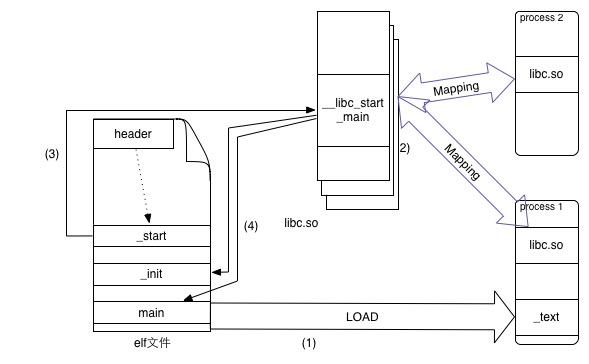
\includegraphics[scale = 0.7]{beforeMain.jpg}
				\caption{进入Main之前操作系统做的事情}
			\end{figure}
			
			\begin{itemize}[itemindent = 1em]
				\item 首先 bash 进行 \verb|fork |系统调用,生成一个子进程,接着在子进程中运行 \verb|execve| 函数指定的 \verb|elf 二进制程序|( Linux中执行二进制程序最终都是通过 \verb|execve| 这个库函数进行的),\verb|execve| 会调用系统调用把 \verb|elf 文件| load 到内存中的代码段(\verb|_text|)中。
				
				\item 如果有依赖的动态链接库,会调用动态链接器进行库文件的地址映射,动态链接库的内存空间是被多个进程共享的。
				
				\item 内核从 \verb|elf| 文件头得到\verb|_start|的地址,调度执行流从\verb|_start|指向的地址开始执行,执行流在\verb|_start|执行的代码段中跳转到\verb|libc|中的公共初始化代码段\verb|__libc_start_main|,进行程序运行前的初始化工作。
				
				\item \verb|__libc_start_main|的执行过程中,会跳转到\verb|_init|中全局变量的初始化工作,随后调用我们的\verb|main|函数,进入到主函数的指令流程。
			\end{itemize}

	

\chapter{正则表达式}
	\section{基础知识}
		\subparagraph{头文件} \verb|#include <regex>|
		
		\subsection{整个字符串是否匹配} \verb|regex_match|
			\begin{lstlisting}
	 regex reg1("\\w+day");
	 string s1 = "saturday";
	 string s2 = "saturday and sunday";
	 smatch r1;
	 smatch r2;
	 cout << boolalpha << regex_match(s1, r1, reg1) << endl;  //true
	 cout << boolalpha << regex_match(s2, r2, reg1) << endl;  //false
	 cout << "s1匹配结果:" << r1.str() << endl;          //saturday
	 cout << "s2匹配结果:" << r2.str() << endl;          //空
	 cout << endl;
			\end{lstlisting}
		\subsection{只返回一个匹配结果} \verb|regex_match|
			\begin{lstlisting}
	smatch rr1;
	smatch rr2;
	cout << boolalpha << regex_search(s1, rr1, reg1) << endl;  //true
	cout << "s1匹配结果:" << rr1.str() << endl;           //saturday
	cout << boolalpha << regex_search(s2, rr2, reg1) << endl;  //true
	cout << "s1匹配结果:" << rr2.str() << endl;           //saturday
	cout << endl;
			\end{lstlisting}
		
		\subsection{返回多个匹配结果} \verb|iterator|
			\begin{lstlisting}
	cout << "iterator结果:" << endl;
	sregex_iterator it(s2.begin(), s2.end(), reg1);
	sregex_iterator end;
	for(; it != end; ++it)
	{
		cout << it->str() << endl;
		//cout << *it << endl; 错误
	}
	
	cout << "token_iterator结果:" << endl;
	sregex_token_iterator tit(s2.begin(), s2.end(), reg1);
	sregex_token_iterator tend;
	for(; tit != tend; ++tit)
	{
		cout << tit->str() << endl;
		cout << *tit << endl;
	}
			\end{lstlisting}
			
	\section{子表达式匹配}
		\begin{lstlisting}
	regex reg2("(\\d{1,3}):(\\d{1,3}):(\\d{1,3}):(\\d{1,3})");
	string ip = "0:11:222:333";
	smatch m; 
	regex_match(ip, m, reg2);
	cout << "输出:str()" << endl;
	cout << m.str() << endl;   //0:11:222:333
	cout << m.str(1) << endl;  //0
	cout << m.str(2) << endl;  //11
	cout << m.str(3) << endl;  //222
	cout << m.str(4) << endl;  //333
	
	cout << "输出:[i]" << endl; //结果同上
	cout << m[0] << endl;
	cout << m[1] << endl;
	cout << m[2] << endl;
	cout << m[3] << endl;
	cout << m[4] << endl;
	
	string ip2 = "0:11:222:333 4:55:66:7";
	sregex_iterator ip_it(ip2.begin(), ip2.end(), reg2);
	sregex_iterator ip_end;
	for(; ip_it != ip_end; ++ip_it)
	{
		cout << ip_it->str() << endl;
		cout << ip_it->str(1) << endl;
		cout << ip_it->str(2) << endl;
		cout << ip_it->str(3) << endl;
		cout << ip_it->str(4) << endl;
	}
		\end{lstlisting}
		
	
\chapter{异常处理}
	\section{简介}
		用于处理软件程序运行时的错误,并用于处理软件系统中可预知或不可预知的问题。这样就可以保证软件系统运行的稳定性与健壮性
		
		C++应用程序中在考虑异常设计时,并不是所有的程序模块处理都需要附加上异常情况的处理。相对来说,异常处理没有普通方法函数调用速度快。过度的错误处理会影响应用程序运行的效率。通常在C++开发的软件系统中,应用程序都由对应的库、组件以及运行的具体不同模块组成。在设计时,异常的处理应充分考虑到独立程序库以及组件之间的情况。便于使用者在程序出现异常情况下,使用库或者组件的开发者能够快速定位出库、组件还是应用程序的错误。
		
		\paragraph{编写流程}
			\begin{enumerate}
				\item 使用Try块
				\item 引发异常
				\item 使用catch 捕获特定类型
			\end{enumerate}
			
		\textbf{try体中可以直接抛出异常,或者在try体中调用的函数体中间接的抛出}
		\begin{lstlisting}
	try
	{
		…               //可能出错产生异常的代码
	
		throwtypen();  //throw  new Type();  一个对象或值
	}catch(type1)
	{
		…               //对应类型的异常处理代码
	}catch(type2)
	{
		…               //对应类型的异常处理代码
	}catch(...) 		//任意类型
	{
	
	}  
	

	或者
	
	try	
	{
		function();//调用可能会抛出异常的函数方法
	}catch(type1)
	{
		…               //对应类型的异常处理代码
	}catch(type2)
	{
		…               //对应类型的异常处理代码
	}	
		\end{lstlisting}

	\section{异常处理机制}
		\subsection{异常再引发}
			\begin{itemize}
			\item 可以在基本任务完成后重新引发所处理的异常,最后再\verb|throw|
			\item 主要用于在程序终止前写入日志和实施特殊的清除任务
			\end{itemize}
			
			\begin{lstlisting}
	try
	{
		throw AnException();
	}
	catch(...)
	{
		..
		throw;
	}
			\end{lstlisting}
			
		\subsection{栈展开}
			\begin{itemize}
				\item  异常引发代码和异常处理程序可能属于不同函数
				\item  当异常发生时,沿着异常处理块的嵌套顺序逆向回溯查找能够处理该异常的catch 字句,即如果当前函数没有处理代码,则返回上一层调用函数查找catch处理代码,以此类推
				\item  如找到对应的catch 字句,处理该异常
				\item  异常处理完后,程序保持catch 字句所在的函数栈框架,不会返回引发异常的函数栈框架,即程序停留在catch处理程序处。
				\item  函数栈框架消失时,局部对象被自动析构,但是如果未执行\verb|delete| 操作,动态分配的目标对象就未被析构
			\end{itemize}
			
			流程如图\ref{process_error}所示
\begin{lstlisting}
	#include <iostream>
	
	using namespace std;
	
	int main()
	{
		try{
			cout << "Before Throw" << endl;
			throw 1; // 抛出对象  new Obj
			cout << "After Throw In Try" << endl;
		}
		catch (int& i)	// 捕获对象 Obj& 
		{
			cout << "After Throw In Catch" << endl;
		}
		
		//如果没有匹配的catch块,就会调用teminate():如果没设置teminate就终止程序..就不会执行下面的语句了
		
		cout << "Main!" << endl;
		cin.get();
	}
\end{lstlisting}
			
			\begin{figure}[h]
				\centering
				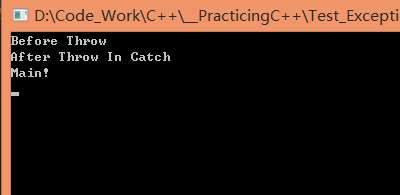
\includegraphics[scale = 1]{Exception_Process.png}
				\caption{流程演示}
				\label{process_error}
			\end{figure}
	
	\subsection{未处理异常}
		\begin{itemize}
			\item 所有未处理异常由预定义函数\verb|std::terminate()| 函数处理
			\item 可以使用\verb|std::set_terminate()| 函数设置\verb|std::terminate()| 函数处理例程。
		\end{itemize}
		
		\begin{lstlisting}
	void term_func()  {  exit( -1 );  }
	int main()
	{
	   try
	   {
	      set_terminate( term_func );
	      throw "Out of memory!";
	   }
	   catch( int ){  /* … */  }
	   return 0;
	}
		\end{lstlisting}
	\subsection{描述函数可否引发异常}
		\begin{itemize}
			\item 声明时,函数后加 \verb|throw()| 表示不能引发异常 等价于 c11\verb|noexcept 或 noexcept(true)|
			\item 声明时,函数后加 \verb|throw(T)| 表示引发某类异常 
			\item 声明时,函数后加 \verb|throw(...)| 表示可以引发任意形式异常 等价于 c11\verb|noexcept(false)|
			\item 可能引发异常 时,c11 使用\verb|noexcept(noexcept(expr))|,expr 为可转换为true  或 false 常数表达式
		\end{itemize}	
		
		c11 建议使用\verb|noexcept| 来表示该函数是否可以抛出异常	
			\begin{lstlisting}
	class JuStack
	{
	  public:
		    JuStack( int cap ) : _stk(new int[cap+1]), _cap(cap), _cnt(0), _top(0)  { }
		    virtual ~JuStack()  {  if( _stk )  delete _stk, _stk = NULL;  }
	  public:
		    int Pop()  throw( EStackEmpty ); // int pop() noexcept(false);
		    void Push( int value )  throw( EStackFull );
		    bool IsFull() const  {  return _cap == _cnt;  }
		    bool IsEmpty() const  {  return _cnt == 0;  }
		    int GetCapacity() const  {  return _cap;  }
		    int GetCount() const  {  return _cnt;  }
  	  private:
		    int * _stk;
		    int _cap, _cnt, _top;
	}; 
	
			\end{lstlisting}
	\subsection{显示异常名字}
		C++ 程序在编译是会将函数名称进行变化,导致战追踪时不好读,此时可以使用 demangle 方法对函数名进行转换,使其回到原先声明的名字,方便阅读差错。
		
\begin{lstlisting}
	// 显示异常 的具体 代码
	#include <exception>
	#include <iostream>
	#include <cxxabi.h>
	
	struct empty { };
	
	template <typename T, int N>
	struct bar { };
	
	
	int main()
	{
		int     status;
		char   *realname;
		
		// exception classes not in <stdexcept>, thrown by the implementation
		// instead of the user
		std::bad_exception  e;
		realname = abi::__cxa_demangle(e.what(), 0, 0, &status);
		std::cout << e.what() << "\t=> " << realname << "\t: " << status << '\n';
		free(realname);
		
		
		// typeid
		bar<empty,17>          u;
		const std::type_info  &ti = typeid(u);
		
		realname = abi::__cxa_demangle(ti.name(), 0, 0, &status);
		std::cout << ti.name() << "\t=> " << realname << "\t: " << status << '\n';
		free(realname);
		
		return 0;
	}
	
	/*
	This prints 
	
	St13bad_exception       => std::bad_exception   : 0
	3barI5emptyLi17EE       => bar<empty, 17>       : 0
	*/
	
\end{lstlisting}	
		\subsection{异常标准库类结构}
			所有的异常类型都继承自std::exception ,在头文件 <exception> 中定义.具体细节见下图:
			\begin{figure}[h]
				\centering
				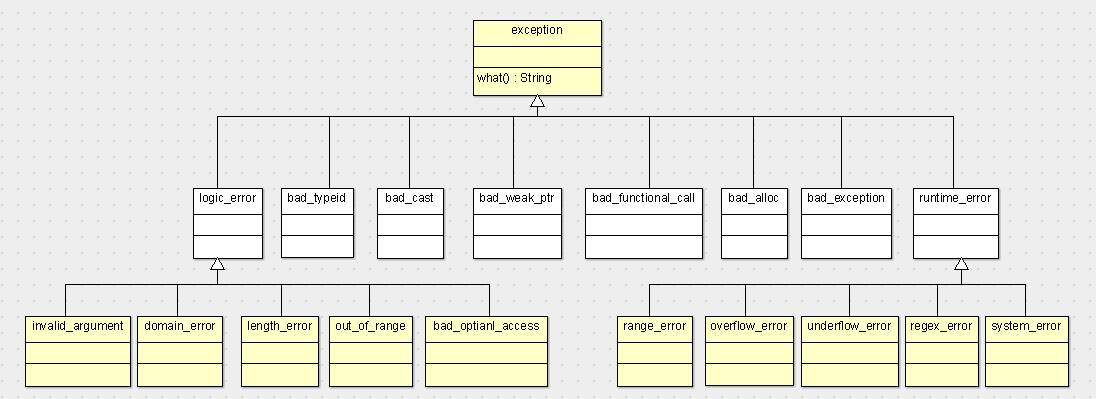
\includegraphics[scale = 0.45]{exception_level.png}
				\caption{Exception 层次结构}
			\end{figure}
	
\begin{lstlisting}
	#include <variant>
	#include <string>
	
	int main()
	{
		std::variant<int, float> v, w;
		v = 12; // v contains int
		int i = std::get<int>(v);
		w = std::get<int>(v);
		w = std::get<0>(v); // same effect as the previous line
		w = v; // same effect as the previous line
		
		//  std::get<double>(v); // error: no double in [int, float]
		//  std::get<3>(v);      // error: valid index values are 0 and 1
		
		try {
			std::get<float>(w); // w contains int, not float: will throw
		}
		catch (std::bad_variant_access&) {}
		
		std::variant<std::string> v("abc"); // converting constructors work when unambiguous
		v = "def"; // converting assignment also works when unambiguous
	}
\end{lstlisting} 
	\section{logic\_error}
		Defines a type of object to be thrown as exception. It reports errors that are a consequence of faulty logic within the program such as violating logical preconditions or class invariants and \textbf{may be preventable.}
		\subsection{invalid\_argument}
			Defines a type of object to be thrown as exception. It reports errors that arise because an argument value has not been accepted.
			
			This exception is thrown by std::bitset::bitset, and the std::stoi and std::stof families of functions. 
		\subsection{domain\_error}
			Defines a type of object to be thrown as exception. It may be used by the implementation to report domain errors, that is, situations where the inputs are outside of the domain on which an operation is defined.
			
			The standard library components do not throw this exception (mathematical functions report domain errors as specified in math\_errhandling). Third-party libraries, however, use this. For example, boost.math throws std::domain\_error if boost::math::policies::throw\_on\_error is enabled (the default setting). 
		\subsection{length\_error}
			Defines a type of object to be thrown as exception. It reports errors that are consequence of attempt to exceed implementation defined length limits for some object.
			
			This exception is thrown by member functions of std::basic\_string and std::vector::reserve 
		\subsection{out\_of\_range}
			Defines a type of object to be thrown as exception. It reports errors that are consequence of attempt to access elements out of defined range.
			
			It may be thrown by the member functions of std::bitset and std::basic\_string, by std::stoi and std::stod families of functions, and by the bounds-checked member access functions (e.g. std::vector::at and std::map::at) 
		\subsection{future\_error}
			The class std::future\_error defines an exception object that is thrown on failure by the functions in the thread library that deal with asynchronous execution and shared states (std::future, std::promise, etc). Similar to std::system\_error, this exception carries an error code compatible with std::error\_code. 
		\subsection{bad\_optional\_access}
			Defines a type of object to be thrown by std::optional::value when accessing an optional object that does not contain a value. 
		
	\section{runtime\_error}
		\subsection{range\_error}
			Defines a type of object to be thrown as exception. It can be used to report range errors (that is, situations where a result of a computation cannot be represented by the destination type)
			
			The only standard library components that throw this exception are std::wstring\_convert::from\_bytes and std::wstring\_convert::to\_bytes.
			
			The mathematical functions in the standard library components do not throw this exception (mathematical functions report range errors as specified in math\_errhandling). 
		\subsection{overflow\_error}
			Defines a type of object to be thrown as exception. It can be used to report arithmetic overflow errors (that is, situations where a result of a computation is too large for the destination type)
			
			The only standard library components that throw this exception are std::bitset::to\_ulong and std::bitset::to\_ullong.
			
			The mathematical functions of the standard library components do not throw this exception (mathematical functions report overflow errors as specified in math\_errhandling). Third-party libraries, however, use this. For example, boost.math throws std::overflow\_error if boost::math::policies::throw\_on\_error is enabled (the default setting). 
		\subsection{underflow\_error}
			Defines a type of object to be thrown as exception. It may be used to report arithmetic underflow errors (that is, situations where the result of a computation is a subnormal floating-point value)
			
			The standard library components do not throw this exception (mathematical functions report underflow errors as specified in math\_errhandling). Third-party libraries, however, use this. For example, boost.math throws std::underflow\_error if boost::math::policies::throw\_on\_error is enabled (the default setting). 
		\subsection{regex\_error}
			Defines the type of exception object thrown to report errors in the regular expressions library. 
\begin{lstlisting}
	#include <regex>
	#include <iostream>
				
	int main()
	{
		try {
			std::regex re("[a-b][a");
		} 
					
		catch (const std::regex_error& e) {
			std::cout << "regex_error caught: " << e.what() << '\n';
			if (e.code() == std::regex_constants::error_brack) {
				std::cout << "The code was error_brack\n";
				}
		}
	}
\end{lstlisting}
		\subsection{system\_error}
			std::system\_error is the type of the exception thrown by various library functions (typically the functions that interface with the OS facilities, e.g. the constructor of std::thread) when the exception has an associated std::error\_code, which may be reported. 
			\subsubsection{ios\_base::failure}
				The class std::ios\_base::failure defines an exception object that is thrown on failure by the functions in the Input/Output library.
				
				std::ios\_base::failure may be defined either as a member class of std::ios\_base or as a synonym (typedef) for another class with equivalent functionality. 
				
\begin{lstlisting}
	#include <iostream>
	#include <fstream>
	int main()
	{
		std::ifstream f("doesn't exist");
		try {
			f.exceptions(f.failbit);
		} catch (const std::ios_base::failure& e)
		{
			std::cout << "Caught an ios_base::failure.\n"
			<< "Explanatory string: " << e.what() << '\n'
			<< "Error code: " << e.code() << '\n';
		}
	}
					
	/*
		Caught an ios_base::failure.
		Explanatory string: ios_base::clear: unspecified iostream_category error
		Error code: iostream:1
	*/
				\end{lstlisting}
			\subsubsection{filesystem::filesystem\_error}
				The class std::filesystem::filesystem\_error defines an exception object that is thrown on failure by the throwing overloads of the functions in the filesystem library. 
				
		\subsection{tx\_exception}
				Defines an exception type that can be used to cancel and roll back an atomic transaction initiated by the keyword atomic\_cancel
					
				If T is not TriviallyCopyable, the program that specializes std::tx\_exception<T> is ill-formed. 
	\section{bad errors}
		\subsection{bad\_typeid}
			An exception of this type is thrown when a typeid operator is applied to a dereferenced null pointer value of a polymorphic type.
			
\begin{lstlisting}
	#include <iostream>
	#include <typeinfo>
	
	struct S { // The type has to be polymorphic
		virtual void f();
	}; 
	
	int main()
	{
		S* p = nullptr;
		try {
			std::cout << typeid(*p).name() << '\n';
		} catch(const std::bad_typeid& e) {
		std::cout << e.what() << '\n';
		}
	}
	
	//Attempted a typeid of NULL pointer!
\end{lstlisting}
		\subsection{bad\_cast}
			\subsubsection{bad\_any\_cast}
				Defines a type of object to be thrown by the value-returning forms of std::any\_cast on failure. 
		\subsection{bad\_weak\_ptr}
			std::bad\_weak\_ptr is the type of the object thrown as exceptions by the constructors of std::shared\_ptr that take std::weak\_ptr as the argument, when the std::weak\_ptr refers to an already deleted object. 
\begin{lstlisting}
	#include <memory>
	#include <iostream>
	int main()
	{
		std::shared_ptr<int> p1(new int(42));
		std::weak_ptr<int> wp(p1);
		p1.reset();
		try {
			std::shared_ptr<int> p2(wp);
		} catch(const std::bad_weak_ptr& e) {
			std::cout << e.what() << '\n';
		}
	}
	
	//std::bad_weak_ptr
\end{lstlisting}
		\subsection{bad\_function\_call}
			std::bad\_function\_call is the type of the exception thrown by std::function::operator() if the function wrapper has no target. 
\begin{lstlisting}
	#include <iostream>
	#include <functional>
	
	int main()
	{
		std::function<int()> f = nullptr;
		try {
			f();
		} catch(const std::bad_function_call& e) {
			std::cout << e.what() << '\n';
		}
	}
	
	//bad function call
\end{lstlisting}
		\subsection{bad\_alloc}
			std::bad\_alloc is the type of the object thrown as exceptions by the allocation functions to report failure to allocate storage
\begin{lstlisting}
	#include <iostream>
	#include <new>
	
	int main()
	{
		try {
				while (true) {
					new int[100000000ul];
				}
			} catch (const std::bad_alloc& e) {
			std::cout << "Allocation failed: " << e.what() << '\n';
		}
	}
	
	//Allocation failed: std::bad_alloc
\end{lstlisting}
		\subsection{bad\_exception}
			std::bad\_exception is the type of the exception thrown by the C++ runtime in the following situations: 
			
			\begin{enumerate}
				\item If a dynamic exception specification is violated and std::unexpected throws or rethrows an exception that still violates the exception specification, but the exception specification allows std::bad\_exception, std::bad\_exception is thrown.
				\item If std::exception\_ptr stores a copy of the caught exception and if the copy constructor of the exception object caught by current\_exception throws an exception, the captured exception is an instance of std::bad\_exception.
			\end{enumerate}

\begin{lstlisting}
	#include <iostream>
	#include <exception>
	#include <stdexcept>
	
	void my_unexp() { throw; }
	
	void test() throw(std::bad_exception)
	{
		throw std::runtime_error("test");
	}
	
	int main()
	{
		std::set_unexpected(my_unexp);
		try {
			test();
		} catch(const std::bad_exception& e)
		{
			std::cerr << "Caught " << e.what() << '\n';
		}
	}
	
	//Caught std::bad_exception
\end{lstlisting}
		\subsection{bad\_variant\_access}
			std::bad\_variant\_access is the type of the exception thrown in the following situations: 
			\begin{itemize}
				\item std::get(std::variant) called with an index or type that does not match the currently active alternative 
				\item  std::visit called to visit a variant that is valueless\_by\_exception 
			\end{itemize}
\begin{lstlisting}
	#include <variant>
	#include <iostream>
	
	int main()
	{
		std::variant<int, float> v;
		v = 12;
		try {
			std::get<float>(v);
		}
		catch(const std::bad_variant_access& e) {
			std::cout << e.what() << '\n';
		}
	}
	
	//bad_variant_access
\end{lstlisting}


%%%%%%%%%%%%%%%%%%%%%%%%%%%%%%%%%%%%%%%%%%%%%%%%%%%%%%%%%%%%%%%%%%%%%%%CHAPTER_MULTITRHEAD%%%%%%%%%%%%%%%%%%%%%%%%%%%%%%%%%%%%%%%%%%%%%%%%%%%%%%%%%%%%%%%%%%%%%%%%%%
\chapter{多线程}
\section{参考}
	多线程使用:\url{http://www.tuicool.com/articles/VFjyYnq}
		
		\url{http://www.2cto.com/kf/201507/419768.html}
		
		\url{http://www.2cto.com/kf/201504/390787.html}
		
		\url{http://blog.jobbole.com/81265/}
	
	内部实现源码:\url{http://blog.jobbole.com/105900/}
	
\section{须知}
	\subsection{线程安全}
		\textbf{线程安全}就是多线程访问时,采用了加锁机制,当一个线程访问该类的某个数据时,进行保护,其他线程不能进行访问直到该线程读取完,其他线程才可使用。不会出现数据不一致或者数据污染。 线程不安全就是不提供数据访问保护,有可能出现多个线程先后更改数据造成所得到的数据是脏数据
		
		比如一个 ArrayList 类,在添加一个元素的时候,它可能会有两步来完成:1. 在 Items[Size] 的位置存放此元素;2. 增大 Size 的值。
		
		在单线程运行的情况下,如果 Size = 0,添加一个元素后,此元素在位置 0,而且 Size=1;
		
		而如果是在多线程情况下,比如有两个线程,线程 A 先将元素1存放在位置 0。但是此时 CPU 调度线程A暂停,线程 B 得到运行的机会。线程B向此 ArrayList 添加元素2,因为此时 Size 仍然等于 0 (注意,我们假设的是添加一个元素是要两个步骤,而线程A仅仅完成了步骤1),所以线程B也将元素存放在位置0。然后线程A和线程B都继续运行,都增加 Size 的值,结果Size等于2。
		那好,我们来看看 ArrayList 的情况,期望的元素应该有2个,而实际只有一个元素,造成丢失元素,而且Size 等于 2。这就是“线程不安全”了
		\subparagraph{线程安全的条件}
			\begin{itemize}
				\item 多个线程同时访问时,其表现出正确的行为。
				\item 无论操作系统怎么调度这些线程,无论这些线程的执行顺序如何交织
				\item 调用端代码 \textbf{无须额外的同步}或其他协调动作。
			\end{itemize}
		\subparagraph{线程安全的类}可以通过 同步原语(类自身拥有的mutex(互斥器)来) 保护内部状态。
		\subparagraph{对象的race condition}这个不能由类自身拥有的mutex(互斥器)来保护,可以借助boost 的shared,weaked ptr 实现的observer 模式解决。
		
		\subsection{对象的创建}
			对象构造时要\textbf{做到}\underline{线程安全},唯一要求是在构造期间不要泄露this指针,即:
				\begin{itemize}
					\item 不要在构造函数中注册任何回调
					\item 不要在构造函数中将this传给跨线程的对象
					\item 即便在最后一行也不行:派生会先执行父类的构造的,而你写的可能就是父类..这样对方就讲返回一个半成品..
				\end{itemize}
\section{概念}
	线程是比进程更小的程序执行单位
	
	多个线程\textbf{可共享全局数据},\textbf{也可使用专有数据}	

	\subparagraph{内核线程}
		\begin{itemize}[itemindent = 1em]
			\item 操作系统内核支持多线程调度与执行
			\item 内核线程使用资源较少,仅包括内核栈和上下文切换时需要的保存寄存器内容的空间
		\end{itemize}
	
	\subparagraph{轻量级进程}
		\begin{itemize}[itemindent = 1em]
			\item 由内核支持的独立调度单元,调度开销小于普通的进程	
			\item 系统支持多个轻量级进程同时运行,每个都与特定的内核线程相关联
		\end{itemize}
	
	\subparagraph{用户线程}
		\begin{itemize}[itemindent = 1em]
			\item 	建立在用户空间的多个用户级线程,映射到轻量级进程后调度执行
			\item   用户线程在用户空间创建、同步和销毁,开销较低
			\item   每个线程具有独特的ID
		\end{itemize}
	
	\subparagraph{进程与线程的比较}
		\begin{itemize}[itemindent = 1em]
			\item 线程空间不独立,有问题的线程会影响其他线程;进程空间独立,有问题的进程一般不会影响其他进程	
			\item 创建进程需要额外的性能开销
			\item 线程用于开发细颗粒度并行性,进程用于开发粗颗粒度并行性
			\item 线程容易共享数据,进程共享数据必须使用进程间通讯机制
		\end{itemize}
	
\section{POSIX线程}
	\subsection{线程创建}
		\subparagraph{线程创建函数}
			\begin{itemize}[itemindent = 1em]
				\item 头文件\verb|"pthread.h"|
				\item 函数 \verb|int pthread_create(pthread_t* thread, const pthread_attr_t* attr, void* (*func)| \verb|(void*), void* arg);|
			\end{itemize}
		\subparagraph{线程创建流程}
			\begin{itemize}[itemindent = 1em]
				\item 定义指向\verb|pthread_t|对象的指针对象,\verb|pthread_t|对象用于存储新线程的\verb|ID|
				\item 定义指向线程属性\verb|pthread_attr_t|对象的指针对象;线程属性对象控制线程与程序其他部分(可能是其他线程)的交互;如果传递\verb|NULL|,则\textbf{使用缺省属性构造新线程}
				
				\item 定义指向线程函数的指针对象,使其指向固定格式的线程函数
				\item 实现线程函数;线程函数的参数和返回值均为哑型指针;\textbf{需要传递多个参数时},打包成单个\verb|void*|型的指针对象
				\item 线程退出时使用返回值将数据传递给主调线程;多个结果同样可以打包传递
			\end{itemize}
			
		\subparagraph{线程创建说明}
			\begin{itemize}[itemindent = 1em]
				\item \verb|pthread_create()|函数在线程创建完毕后立即返回,它并不等待线程结束
				\item 原线程与新线程如何执行与调度有关,程序不得依赖线程先后执行的关系
				\item 可以使用同步机制确定线程的先后执行关系
			\end{itemize}
			
		\subparagraph{线程退出方式}
			\begin{itemize}[itemindent = 1em]
				\item 线程函数结束执行
				\item 调用\verb|pthread_exit()|函数显式结束
				\item 被其他线程撤销
			\end{itemize}
			
		\subparagraph{示例代码}\verb|->|
		
			\begin{lstlisting}
	#include <pthread.h> 
	#include <iostream>
	void *  PrintAs( void * unused )
	{
		while( true )    std::cerr << 'a';
		return NULL;
	}
	void *  PrintZs( void * unused )
	{
		while( true )    std::cerr << 'z';
		return NULL;
	}
	int  main()
	{
		pthread_t  thread_id;
		pthread_create( &thread_id, NULL, &PrintAs, NULL );
		PrintZs( NULL );
		return 0;
	}
	
			\end{lstlisting}
		
	\subsection{线程ID}
	
	\subsection{线程属性}
	
	\subsection{线程撤销}

	\subsection{线程局部存储}
	
	\subsection{线程清除}
			
\section{C++11线程}
	\subsection{头文件}
		\begin{itemize}
			\item \verb|<atomic>|: 包含\verb|std::atomic|和\verb|std::atomic_flag|类,以及一套C风格的原子类型和与C兼容的原子操作的函数。
			\item \verb|<thread>|: 包含\verb|std::thread|类以及\verb|std::this_thread|命名空间。
			\item \verb|<mutex>|: 包含与互斥量(\verb|mutex、lock_guard、unique_lock|)相关的类以及其他类型和函数。
			\item \verb|<condition_variable>|: 包含与条件变量相关的类, 包括\verb|std::condition_variable |和
			
			 \verb|std::condition_variable_any|。
			\item \verb|<future>|:包含两个\verb|Promise|类(\verb|std::promise|和\verb|std::package_task|)和两个\verb|Future|类(\verb|std::future|和\verb|std::shared_future|)以及相关的类型和函数
		\end{itemize}

	\subsection{线程类}
		首先其类模板模型如下图所示:
		\begin{figure}[h]
			\centering
			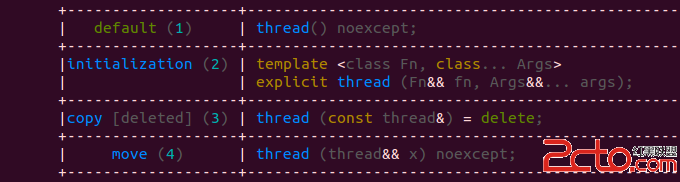
\includegraphics[scale= 0.8]{thread.png}
			\caption{Thread Pattern}
		\end{figure}
		\begin{lstlisting}
	namespace std
	{
		struct thread
		{
			// native_handle_type 是连接 thread 类和操作系统 SDK API 之间的桥梁。
			typedef implementation-dependent native_handle_type;
			native_handle_type native_handle();
			// 线程ID
			struct id
			{
				id() noexcept;
				// 可以由==, < 两个运算衍生出其它大小关系运算。
				bool operator==(thread::id x, thread::id y) noexcept;
				bool operator<(thread::id x, thread::id y) noexcept;
				template<class charT, class traits>
				basic_ostream<charT, traits>&
				operator<<(basic_ostream<charT, traits>&out, thread::id id);
				// 哈希函数
				template <class T> struct hash;
				template <> struct hash<thread::id>;
			};
			id get_id() const noexcept;
			// 构造与析构
			thread() noexcept;
			// 注意:前面为函数,后面为函数的参数表..的实参值.
			template<class F, class… Args> explicit thread(F&f, Args&&… args);
			~thread();
			thread(const thread&) = delete;
			thread(thread&&) noexcept;
			thread& operator=( const thread&) = delete;
			thread& operator=(thread&&) noexcept;
			//
			void swap(thread&) noexcept;
			bool joinable() const noexcept; //判断线程是否可联
			void join();  //等待线程结束
			void detach(); //分离线程
			// 获取物理线程数目
			static unsigned hardware_concurrency() noexcept;
		}
		
		namespace this_thead
		{
			thread::id get_id();
			void yield();
			// 阻塞当前线程至指定时点
			template<class Clock, class Duration>
			void sleep_until(const chrono::time_point<Clock, Duration>& abs_time);
			// 阻塞当前线程指定时长
			template<class Rep, class Period>
			void sleep_for(const chromo::duration<Rep, Period>& rel_time);
		}
	}	
		\end{lstlisting}
		
	\subparagraph{初始化方式..}
		创建如果指定函数,那么创建成功后就立刻执行,否则等待函数指定时执行。
		
		\verb|join| 函数用于等待结束。
		
		线程局部存储使用\verb|thread_local|关键字
		
		\begin{enumerate}[itemindent = 1em]
			\item \verb|thread_run_func_var_args|:
			\begin{lstlisting}
	#include <iostream>
	#include <thread>
			
	using namespace std;
			
	void myFirstThreadTask(int num)
	{
		for (int i = 0; i < 10; ++i)
		{
			cout << "myFirstThreadTask's num = " << num++ << endl;
			this_thread::sleep_for(chrono::milliseconds(10));
		}
	}
			
	void mySecondThreadTask(int &num)
	{
		for (int i = 0; i < 10; ++i)
		{
			cout << "mySecondThreadTask's num = " << num++ << endl;
			this_thread::sleep_for(std::chrono::milliseconds(10));
		}
	}
			
	int _tmain(int argc, _TCHAR* argv[])
	{
		int n = 5;
		thread myThread0;//myThread1为一个空线程,不代表任何可执行对象
			
		//myThread1与myFirstThreadTask函数绑定,n为其按值传递参数
		thread myThread1(myFirstThreadTask,n);
			
		//myThread2与mySecondThreadTask函数绑定,n为其引用传递参数
		thread myThread2(mySecondThreadTask,std::ref(n));
		myThread1.join();
		myThread2.join();
			
		n++;
			
		//现在myThread2不代表任何可执行对象,myThread3与mySecondThreadTask函数绑定
		thread myThread3(std::move(myThread2));
		//myThread3.join();
		return 0;
	}
			\end{lstlisting}
			\item \verb|thread_run_lambda|:
			\begin{lstlisting}
	void threadRunLambda(void)
	{
		int a = 100,
		b = 200;
		thread* t = new thread( 
		[](int ia, int ib)
		{
		cout << (ia + ib) << endl;
		},
		a,
		b );
			
		t->join();
		delete t;
	}
			\end{lstlisting}
			\item \verb|thread_run_member_func|:
			\begin{lstlisting}
// Method1:
	struct God
	{
		void create(string& anything)
		{
			cout << "create " << anything << endl;
		}
	};
			
	void threadRunMemberFunction(void)
	{
		God god;
		string s = "some";
		thread* t = new thread( &God::create, god, s );// 虽然函数定义为引用,但是还是值传递参数,如果需要引用,需要添加std::ref(s);
		// t = new thread(&God::create,god,std::ref(s)); 这样才会真正的引用传递参数
		t->join();
		delete t;
	}

// Method2:
	class Factor{
	public:
		void operater() (int a){
			cout <<"create"<< a <<endl;
		}
	};

	void threadRunObject(void)
	{
		Factor factor;
		int a = 1;
		
		thread t(factor, a);
		thread t2(Factor(),a)
		t.join();
		t2.join();
	}
			\end{lstlisting}
			
			\item  \verb|bind()将函数转化为return Type(*pointer)()|
				\begin{lstlisting}
	#include <iostream>
	#include <thread>
	class Worker  {
		public:
		Worker( int a = 0, int b = 0 ) : _a(a), _b(b)  {  }
		void  ThreadFunc()  {  ……  }
		private:  int  _a, _b;
	};
	
	int  main()
	{
		Worker  worker( 10, 20 );
		std::thread  t( std::bind( &Worker::ThreadFunc, &worker ) );
		t.join();
		return 0;
	}
				\end{lstlisting}
		\end{enumerate}
		
	\subsection{线程间数据交互和数据争用(Data Racing)}
		同一个进程内的多个线程之间多是免不了要有数据互相来往的,队列和共享数据是实现多个线程之间的数据交互的常用方式,封装好的队列使用起来相对来说不容易出错一些,而共享数据则是最基本的也是较容易出错的,因为它会产生数据争用的情况,即有超过一个线程试图同时抢占某个资源,比如对某块内存进行读写等,如下例所示:
		\begin{lstlisting}
static void inc(int *p)
{
	for(int i = 0; i < COUNT; ++i)
	(*p)++;
}
		
void ThreadDataRacing()
{
	int a = 0;
	thread th1(inc, &a);
	thread th2(inc, &a);
		
	th1.join();
	th2.join();
		
	cout<<"a = "<<a<<endl;
}
		\end{lstlisting}
		
		这是简化了的极端情况,我们可以一眼看出来这是两个线程在同时对\&a 这个内存地址进行写操作,但是在实际工作中,在代码的海洋中发现它并不一定容易。从表面看,两个线程执行完之后,最后的 a 值应该是 COUNT * 2,但是实际上并非如此,\textbf{因为简单如 (*p)++这样的操作并不是一个原子动作,要解决这个问题,对于简单的基本类型数据如字符、整型、指针等,C++提供了原子模版类 atomic},\underline{而对于复杂的对象},\textbf{则提供了最常用的锁机制,比如互斥类 mutex,门锁 lock\_guard,唯一锁 unique\_lock,条件变量 condition\_variable 等}。
		
		\subparagraph{解决方案:}
		\begin{enumerate}[itemindent = 1em]
			\item \textbf{atomic}:针对简单的基本类型数据如\textbf{字符、整型、指针}等 
			\begin{lstlisting}
static void inc(atomic<int> *p )
{
	for(int i = 0; i < COUNT; i++)
	{
		(*p)++;
	}
}
void threadDataRacing(void)
{
	atomic<int> a(0) ;
				
	thread ta( inc, &a);
	thread tb( inc, &a);
				
	ta.join();
	tb.join();
				
	cout << "a=" << a << endl;
}
			\end{lstlisting}
			\item \textbf{lock\_guard}:lock\_guard 是一个\textbf{范围锁},本质是 RAII(Resource Acquire Is Initialization),在构建的时候自动加锁,在析构的时候自动解锁,这保证了每一次加锁都会得到解锁。即使是调用函数发生了异常,在清理栈帧的时候也会调用它的析构函数得到解锁,从而保证每次加锁都会解锁,但是我们不能手工调用加锁方法或者解锁方法来进行更加精细的资源占用管理
			\begin{lstlisting}
static mutex g_mutex;
static void inc(int *p )
{
	for(int i = 0; i < COUNT; i++)
	{
	lock_guard<mutex> _(g_mutex);
		(*p)++;
	}
}
			
void threadLockGuard(void)
{
	int a = 0;
			
	thread ta( inc, &a);
	thread tb( inc, &a);
			
	ta.join();
	tb.join();
			
	cout << "a=" << a << endl;
}
			\end{lstlisting}
			\item \textbf{mutex}:如果要\textbf{支持手工加锁},可以考虑使用 unique\_lock 或者直接使用 mutex。unique\_lock 也支持 RAII,它也可以一次性将多个锁加锁;如果使用 mutex 则直接调用 mutex 类的 lock, unlock, trylock 等方法进行更加精细的锁管理
			
			Mutual exclusion algorithms \textbf{prevent} multiple threads from simultaneously accessing shared resources. This prevents data races and provides support for synchronization between threads.
			\begin{lstlisting}
static mutex g_mutex;
static void inc(int *p )
{
	thread_local int i; // TLS 变量
	for(; i < COUNT; i++)
	{
		g_mutex.lock();
		(*p)++;
		g_mutex.unlock();
	}
}
			
void threadMutex(void)
{
	int a = 0;
			
	thread ta( inc, &a);
	thread tb( inc, &a);
			
	ta.join();
	tb.join();
	cout << "a=" << a << endl;
}
			\end{lstlisting}
			
			在上例中,我们还使用了\textbf{线程本地存储 (TLS) 变量},我们只需要在变量前面声明它是 \verb|thread_local| 即可。\textit{TLS 变量在线程栈内分配,线程栈只有在线程创建之后才生效,在线程退出的时候销毁},需要注意不同系统的线程栈的大小是不同的,如果 TLS 变量占用空间比较大,需要注意这个问题。TLS 变量一般不能跨线程,其初始化在调用线程第一次使用这个变量时进行,默认初始化为 0。
			
			\item \textbf{conditon\_variable}: 对于线程间的事件通知,提供了条件变量类 \verb|condition_variable|,可视为 \verb|pthread_cond_t| 的封装,使用条件变量可以让一个线程等待其它线程的通知 (\verb|wait|,\verb|wait_for|,\verb|wait_until|),也可以给其它线程发送通知 (\verb|notify_one|,\verb|notify_all|),条件变量必须和锁配合使用,在等待时因为有解锁和重新加锁,所以,在等待时必须使用可以手工解锁和加锁的锁,比如 \verb|unique_lock|,而不能使用 \verb|lock_guard|
			
			\begin{lstlisting}
#include <condition_variable>
mutex m;
condition_variable cv;
void threadCondVar(void)
{
	# define THREAD_COUNT 10
	thread** t = new thread*[THREAD_COUNT];
	int i;
	for(i = 0; i < THREAD_COUNT; i++)
	{
		t[i] = new thread( [](int index){
			unique_lock<mutex> lck(m);
			cv.wait_for(lck, chrono::hours(1000));
			cout << index << endl;
			}, i );
			
		this_thread::sleep_for( chrono::milliseconds(50));
	}
	for(i = 0; i < THREAD_COUNT; i++)
	{
		lock_guard<mutex> _(m);
		cv.notify_one();
	}
	for(i = 0; i < THREAD_COUNT; i++)
	{
		t[i]->join();
		delete t[i];
	}
	delete t;
}
			\end{lstlisting}
		\end{enumerate}
	\subsection{互斥锁}
		多线程编程一般避免不了同步的问题,C++11这里也提供了非常方便的方法来进行解决。标准中提供了一下四种互斥锁,分别是:
		\begin{itemize}
			\item  \textbf{Mutex}:基本的Mutex类,\textbf{独占的互斥量,不能递归使用},提供了核心函数lock()和unlock()
			\item  \textbf{Recursive\_mutex}:递归Mutex类,允许在同一个线程中对一个互斥量的多次加锁与解锁操作。一般在项目模块分工中可以使用,这样即使其他人使用了同样的锁也不会导致死锁
			\item \textbf{Timed\_mutex}:定时递归Mutex类,\textbf{带超时的独占的互斥量,不能递归使用},除了递归,还可以在某个时间段里或者某个时刻到达之间获取该互斥量。当一个线程在临界区操作的时间非常长,可以用定时锁指定时间
			\item \textbf{Recursive\_timed\_mutex}:定时递归Mutex类,\textbf{带超时的递归互斥量},综合timed\_mutex和recuseive\_mutex
		\end{itemize}
		
		下面是一个使用基本锁的小例子,该程序会按顺序输出5对enter和leave,分别对应5个线程。如果注释掉函数f中mt的lock和unlock函数,则线程没有同步,此时先输出5句enter,然后5s后再输出5句leave.
		\subsubsection{Mutex}
			\begin{lstlisting}
	#include <iostream>
	#include <thread>
	#include <string>
	#include <mutex>
	#include <vector>
	using namespace std;
	
	mutex mt; //注意,全局的哟..
	
	void f()
	{
		mt.lock();
		cout << "Enter Critical Section" << endl;
		this_thread::sleep_for(chrono::seconds(5));
		cout << "Leave Critical Section" << endl;
		mt.unlock();
	}
	
	int main()
	{
		vector<thread> v(5);
		for (auto &i : v) i = thread(f);
		for (auto &i : v) i.join();
	}
		\end{lstlisting}
		\subparagraph{lock\_guard<T\_mutex> m(T\_mutex)}:从对象初始化时 到 对象销毁时,所有权不可转移,对象生存期内不允许手动加锁和解锁
		
		
		\subparagraph{unique\_lock<T\_mutex> m(T\_mutex)}:提供比lock\_guard 更灵活的方式,可以指定什么时候上锁,什么时候解锁,但是可以保证任何时候都会在析构时将锁释放掉。
			\begin{lstlisting}
void func()
{
	// 当作用域为函数的全部作用域时,lock_guard 与 unique_lock 起到了同样的作用
	lock_guard<std::mutex>locker(mutex);
	unique_lock<std::mutex>locker2(mutex2);
	
	// 但是在申请锁的时候不想上锁,lock_guard 就不行了,这是unique_lock 可以这样做
	unique_lock<std::mutex>locker3(mutex3, std::defer_lock);
		...stuff
		locker3.lock();
		...stuff..
		// 在处理玩这些事之后 就不需要锁了,unique 可以unlock()
		locker3.unlock();
		...stuff
		// 又需要了
		locker3.lock();
		
		// 而且unique_lock 可以被移动,而lock_guard 不可以,但是两者都不可以复制	
		unique_lock<std::mutex> locker4 = std::move(locker3);	
}	
			\end{lstlisting}
		\subparagraph{Recursice\_mutex}
			为什么需要使用 Recursive\_mutex,看例子
			\begin{lstlisting}
struct Complex {
	std::mutex mutex;
	int i;
	
	Complex() : i(0) {}
	
	void mul(int x){
		std::lock_guard<std::mutex> lock(mutex);
		i *= x;
	}
	
	void div(int x){
		std::lock_guard<std::mutex> lock(mutex);
		i /= x;
	}
	
	void both(int x, int y){
		std::lock_guard<std::mutex> lock(mutex);
		mul(x);
		div(y);
	}
};	
	
int main(){
	Complex complex;
	complex.both(32, 23);
	
	return 0;
}

//If you launch this application, you'll see that the program will never terminates. The problem is very simple. In the both() function, the thread acquires the lock and then calls the mul() function. In this function, the threads tries to acquire the lock again, but the lock is already locked. This is a case of deadlock. By default, a thread cannot acquire the same mutex twice.
			\end{lstlisting}
		
			\textbf{There is a simple solution to this problem: std::recursive\_mutex}. This mutex can be acquired several times by the same thread.
			\begin{lstlisting}
struct Complex {
	std::recursive_mutex mutex;
	int i;
	
	Complex() : i(0) {}
	
	void mul(int x){
		std::lock_guard<std::recursive_mutex> lock(mutex);
		i *= x;
	}
	
	void div(int x){
		std::lock_guard<std::recursive_mutex> lock(mutex);
		i /= x;
	}
	
	void both(int x, int y){
		std::lock_guard<std::recursive_mutex> lock(mutex);
		mul(x);
		div(y);
	}
};	

//This time, the application works correctly.		
			\end{lstlisting}
	\subsubsection{Call once}
		Sometimes \textbf{you want a function to be called only once no matter the number of threads that are used}. Imagine a function that has two parts. The first part has to be called only once and the second has to be executed every time the function gets called. We can use the std::call\_once function to fix this problem very easily.
		
		\begin{lstlisting}
std::once_flag flag;

void do_something(){
	std::call_once(flag, [](){std::cout << "Called once" << std::endl;});
	
	std::cout << "Called each time" << std::endl;
}

int main(){
	std::thread t1(do_something);
	std::thread t2(do_something);
	std::thread t3(do_something);
	std::thread t4(do_something);
	
	t1.join();
	t2.join();
	t3.join();
	t4.join();
	
	return 0;
}			
		\end{lstlisting}
	\subparagraph{注意:}
		\begin{enumerate}[itemindent = 1em]
			\item 多次获取互斥量可能会发生死锁,所以我们调用std::recursive\_mutex递归锁,允许同一线程多次获得该锁,\textbf{一般不要使用递归锁},原因:
				\begin{itemize}
					\item 用到递归锁会使得程序的逻辑变复杂,使用到递归锁的程序一般可以简化
					\item 递归锁比非递归锁效率低
					\item 递归锁的可重入次数是有限的,超过也会报错
				\end{itemize}
			\item 可以使用带超时时间的互斥锁,避免阻塞在等待互斥锁上
			\item unique\_lock: 是一个通用的互斥量封装类。与lock\_guard不同,它还支持延迟加锁、时间锁、递归锁、锁所有权的转移并且还支持使用条件变量。这也是一个不可复制的类,但它是可以移动的类
		\end{enumerate}
		
		Keep in mind that \textbf{locks are slow}. Indeed, when you use locks you make sections of the code sequential. \textbf{If you want an highly parallel application}, there are other solutions than locks that are performing much better.
	\subsection{条件变量}
		\subparagraph{condition\_variable}\verb|->|
		
			\textbf{必须}与\verb|std::unique_lock|配合使用
		
			条件变量condition\_variable\textit{也可以}\textbf{进行线程之间的通信},\textit{当一个线程要等待另一个线程完成某个操作时},\textbf{可以使用条件变量进行实现}。\textit{条件变量可以将一个或多个线程进入阻塞状态,直到收到另外一个线程的通知,或者超时才能退出阻塞状态}。
			
			\textbf{一个线程等待某个条件满足},其首先获得一个\verb|unique_lock|锁。该锁将会传递给\verb|wait()|方法,然后\verb|wait()|方法会释放互斥量并将该线程暂停,\textbf{直到条件变量得到相应的信号}。当接受到信号,线程被唤醒后,该锁就又被重新获得了。
			
			\textbf{另外一个线程发送信号使得条件满足}。其通过调用\verb|notify_one()|来发送通知,会将处于阻塞状态的等待该条件获得信号的线程中的某一个线程(\textbf{任意一个线程)恢复执行};还可以通过调用\verb|notify_all()|将\textbf{等待该条件的所有线程唤醒}。

			\begin{lstlisting}
#include <iostream>
#include <thread>
#include <mutex>
#include <condition_variable>
std::mutex  x;
std::condition_variable  cond;
bool  ready = false;
bool  IsReady()  {  return ready;  }
void  Run( int no )
{
	std::unique_lock<std::mutex>  locker( x );
	while( !ready )		//  若标志位非true,阻塞当前线程
	cond.wait( locker );	//  解锁并睡眠,被唤醒后重新加锁
	//  以上两行代码等价于cond.wait( locker, &IsReady );
	//  第二个参数为谓词,亦可使用函子实现
	std::cout << "thread " << no << '\n';
}

int  main()
{
	std::thread  threads[8];
	for( int i = 0; i < 8; ++i )
	threads[i] = std::thread( Run, i );
	std::cout << "8 threads ready...\n";
	{
		std::unique_lock<std::mutex>  locker( x );    //  互斥加锁
		ready = true;		//  设置全局标志位为true
		cond.notify_all();	//  唤醒所有线程
	}    //  离开作用域,自动解锁;可将此复合语句块实现为函数
	//  基于区间的循环结构,对属于threads数组的所有元素t,执行循环体
	for( auto & t: threads )
		t.join();
	return 0;
}
		\end{lstlisting}
		
		\subparagraph{conditon\_variable\_any} \verb|->|
		
		更加通用的条件变量,可以与任意型式的互斥锁配合使用,相比前者使用时会有额外的开销
		
	\subsection{期许与承诺}
		\paragraph{线程的返回值}
			为支持跨平台,thread 类无属性字段保存线程函数的返回值。解决方案有三种:
			\begin{itemize}[itemindent = 2em]
				\item 使用指针类型的函数参数
				\item 使用期许\verb|std::future| 类模版
				\item 使用承诺\verb|std::promise|类模版
			\end{itemize}	
	
		\subsubsection{指针型式参数}
			使用指针作为函数参数,获取线程计算结果
			
			\begin{lstlisting}
#include <iostream>
#include <vector>
#include <tuple>
#include <thread>
#include <mutex>
std::mutex x;
//  劳工线程类模板,处理T型数据对象
template< typename T >  class Worker
{
public:
	explicit Worker( int no, T a = 0, T b = 0 ) : _no(no), _a(a), _b(b)  {  }
	void  ThreadFunc( T * r )  {  x.lock();    *r = _a + _b;    x.unlock();  }
private:
	int  _no;	//  线程编号,非线程ID
	T  _a, _b;	//  保存在线程中的待处理数据
};
		
int main()
{
	//  定义能够存储8个三元组的向量v,元组首元素为指向劳工对象的指针
	//  次元素保存该劳工对象计算后的结果数据,尾元素为指向劳工线程对象的指针
	//  向量中的每个元素都表示一个描述线程运行的线程对象,
	//  该线程对象对应的执行具体任务的劳工对象,及该劳工对象运算后的返回值
	std::vector< std::tuple<Worker<int>*, int, std::thread*> >  v( 8 );
			
	//  构造三元组向量,三元编号顺次为0、1、2
	for( int i = 0; i < 8; i++ )
		v[i] = std::make_tuple( new Worker<int>( i, i+1, i+2 ), 0, nullptr );
			
	//  输出处理前结果;使用std::get<n>(v[i])获取向量的第i个元组的第n个元素
	//  三元编号顺次为0、1、2,因而1号元保存的将是劳工对象运算后的结果
	for( int i = 0; i < 8; i++ )
		std::cout << "No. " << i << ": result = " << std::get<1>(v[i]) << std::endl;
	//  创建8个线程分别计算
	for( int i = 0; i < 8; i++ )
	{
		//  将劳工类成员函数绑定为线程函数,对应劳工对象绑定为执行对象
		//  将构造线程对象时传递的附加参数作为被绑定的线程函数的第一个参数
		//  auto表示由编译器自动推断f的型式
		auto  f = std::bind( &Worker<int>::ThreadFunc,
		std::get<0>( v[i] ), std::placeholders::_1 );
				
		//  动态构造线程对象,并保存到向量的第i个三元组中
		//  传递三元组的1号元地址,即将该地址作为线程函数的参数
		//  线程将在执行时将结果写入该地址
		//  此性质由绑定函数std::bind()使用占位符std::placeholders::_1指定
		//  线程对象为2号元,即三元组的最后一个元素
		std::get<2>( v[i] ) = new std::thread( f, &std::get<1>( v[i] ) );
	}
	for( int i = 0; i < 8; i++ )
	{
		//  等待线程结束
		std::get<2>( v[i] )->join(); 
		//  销毁劳工对象
		delete std::get<0>( v[i] ),    std::get<0>( v[i] ) = nullptr;
		//  销毁线程对象
		delete std::get<2>( v[i] ),    std::get<2>( v[i] ) = nullptr;
	}
			
	//  输出线程计算后的结果
	for( int i = 0; i < 8; i++ )
		std::cout << "No. " << i << ": result = " << std::get<1>(v[i]) << std::endl;
	return 0;
}	   				
			\end{lstlisting}
				
		\subsubsection{期许future}\verb|->|
		
			\textbf{目的}:\textbf{获取异步操作结果},延迟引发线程的异步操作异常
			
			\textbf{使用方法}:
				\begin{itemize}[itemindent = 2em]
					\item 定义期许模板类的期许对象
					\item 使用\verb|std::async()|函数的返回值初始化
					\item 调用期许对象的成员函数\verb|get()|获取线程返回值
				\end{itemize}
			
			\verb|使用期许对象获取线程返回值|
			\begin{lstlisting}
#include <iostream>
#include <exception>
#include <thread>
#include <future>
	
unsigned long int  CalculateFactorial( short int n )
{
	 unsigned long int  r = 1;
	 if( n > 20 )
		 throw std::range_error( "The number is too big." );
	 for( short int i = 2; i <= n; i++ )
		 r *= i;
	return r;
}

int main()
{
	short int  n = 20;
	//  启动异步线程,执行后台计算任务,并返回std::future对象
    std::future<unsigned long int>  f = std::async( CalculateFactorial, n );
    try
    {
        //  获取线程返回值,若线程已结束,立即返回,否则等待该线程计算完毕
        //***(重点)  若线程引发异常,则延迟到std::future::get()或std::future::wait()调用时引发,   在调用端处理异常
	    unsigned long int  r = f.get();
	    std::cout << n << "! = " << r << std::endl;
	}
	catch( const std::range_error & e )  
	{
	    std::cerr << e.what() << std::endl;
    }
  return 0;
}
	
			\end{lstlisting}
			
			\subparagraph{理论}	
			\verb|std::future|可以用来\textbf{获取异步任务的结果},因此可以把它当成一种简单的线程间同步的手段。\verb|std::future| 通常\textbf{由某个 Provider 创建},你可以把 Provider 想象成一个异步任务的提供者,\textbf{Provider 在某个线程中设置共享状态的值},\textbf{与该共享状态相关联的} \verb|std::future| \textbf{对象调用} \verb|get|\textbf{(通常在另外一个线程中) 获取该值},\textit{如果共享状态的标志不为 ready,则调用 std::future::get 会阻塞当前的调用者,直到 Provider 设置了共享状态的值(此时共享状态的标志变为 ready)},\verb|std::future::get| \textbf{返回}异步任务的\textbf{值或异常}(如果发生了异常)。
						
			一个有效(valid)的 \verb|std::future| 对象通常由以下三种 Provider 创建,并和某个共享状态相关联。Provider 可以是函数或者类,其实我们前面都已经提到了,他们分别是:
				\begin{itemize}
					\item \textbf{std::async} 函数
					\item \textbf{std::promise::get\_future},get\_future 为 promise 类的成员函数
					\item \textbf{std::packaged\_task::get\_future},此时 get\_future为 packaged\_task 的成员函数
				\end{itemize}

			一个 \verb|std::future| 对象只有在有效(valid)的情况下才有用(useful),由 \verb|std::future| 默认构造函数创建的 future 对象不是有效的(除非当前非有效的 future 对象被 move 赋值另一个有效的 future 对象)。
			
			在一个有效的 \verb|future| 对象上调用 \verb|get| 会阻塞当前的调用者,直到 Provider 设置了共享状态的值或异常(此时共享状态的标志变为 ready),\verb|std::future::get| 将返回异步任务的值或异常(如果发生了异常)。
\begin{lstlisting}
#include <iostream>       // std::cout
#include <future>         // std::async, std::future
#include <chrono>         // std::chrono::milliseconds

// a non-optimized way of checking for prime numbers:
bool is_prime (int x) 
{
	for (int i=2; i<x; ++i) if (x%i==0) return false;
	return true;
}

int main ()
{
	// call function asynchronously:
	std::future<bool> fut = std::async (is_prime,444444443); 
	
	// do something while waiting for function to set future:
	std::cout << "checking, please wait";
	std::chrono::milliseconds span (100);
	while (fut.wait_for(span)==std::future_status::timeout)
		std::cout << '.' << std::flush;
	
	bool x = fut.get();     // retrieve return value
	
	std::cout << "\n444444443 " << (x?"is":"is not") << " prime.\n";
	
	return 0;
}

//checking, please wait........................
//444444443 is prime.
\end{lstlisting}			
	
		\subsubsection{承诺promise}\verb|->|
				
					\textbf{目的}:承诺对象\textbf{允许}期许对象\textbf{获取}线程对象创建的\textbf{线程返回值}

					\textbf{使用方法}:
						\begin{itemize}[itemindent = 2em]
							\item 创建承诺\verb|std::promise<T>|对象
							
							\item 获取该承诺对象的\textbf{相关}期许\verb|std::future<T>|对象
							
							\item 创建线程对象,并传递承诺对象
							
							\item 线程函数内部通过承诺模板类的成员函数\verb|set_value()|、\verb|set_value_at_thread_exit()|、\verb|set_exception()|或\verb|set_exception_at_thread_exit()|设置值或异常
							
							\item 通过期许对象等待并获取异步操作结果
							
						\end{itemize}
					
					\verb|使用承诺对象获取线程返回值|	
					\begin{lstlisting}
#include <iostream>
#include <exception>
#include <thread>
#include <future>

unsigned long int CalculateFactorial( short int n )
{
  unsigned long int r = 1;
  if( n > 20 )    
	  throw std::range_error( "The number is too big." );
  for( short int i = 2; i <= n; i++ )    
	  r *= i;
  return r;
}

//  CalculateFactorial()函数的包装函数原型
void DoCalculateFactorial(std::promise<unsigned long int> && promise, short int n );

int main()
{
    short int  n = 6;
    std::promise<unsigned long int>  p;    //  创建承诺对象
    std::future<unsigned long int>  f = p.get_future();    //  获取相关期许对象
    //  启动线程,执行CalculateFactorial()函数的包装函数
    std::thread  t( DoCalculateFactorial, std::move( p ), n );
    t.detach();
    try
    {
      unsigned long int  r = f.get();
      std::cout << n << "! = " << r << std::endl;
    }
    catch( std::range_error & e )
      std::cerr << e.what() << std::endl;
  return 0;
}



// 重点
// CalculateFactorial()函数的包装函数实现
void DoCalculateFactorial(std::promise<unsigned long int> && promise, short int n )
{
	  try
	  {
		    //  设置线程返回值,供期许对象获取
		    promise.set_value( CalculateFactorial( n ) );
	  }
	  catch( ... )
	  {
		    //  捕获全部异常,并在期许获取线程返回值时重新引发
		    promise.set_exception( std::current_exception() );
	  }
}

					\end{lstlisting}
	
			\subparagraph{理论}
			\verb|promise |对象可以保存某一类型 \verb|T| 的值,该值可被 \verb|future| 对象读取(可能在另外一个线程中),因此 \verb|promise| 也提供了一种线程同步的手段。在 \verb|promise| 对象构造时可以和一个共享状态(通常是\verb|std::future|)相关联,并可以在相关联的共享状态(\verb|std::future|)上保存一个类型为\verb| T| 的值。
			
			可以通过 \verb|get_future| 来获取与该 \verb|promise| 对象相关联的 \verb|future| 对象,调用该函数之后,两个对象共享相同的共享状态(shared state)
				\begin{itemize}
					\item \textbf{promise} 对象是异步 Provider,它可以在某一时刻设置共享状态的值。
					\item \textbf{future} 对象可以异步返回共享状态的值,或者在必要的情况下阻塞调用者并等待共享状态标志变为 ready,然后才能获取共享状态的值。
				\end{itemize}
			
			下面以一个简单的例子来说明上述关系
				\begin{lstlisting}
void print_int(std::future<int>& fut) {
	int x = fut.get(); // 获取共享状态的值.
	std::cout << "value: " << x << '\n'; // 打印 value: 10.
}

int main ()
{
	std::promise<int> prom; // 生成一个 std::promise<int> 对象.
	std::future<int> fut = prom.get_future(); // 和 future 关联.
	std::thread t(print_int, std::ref(fut)); // 将 future 交给另外一个线程t.
	prom.set_value(10); // 设置共享状态的值, 此处和线程t保持同步.
	t.join();
	return 0;
}					
				\end{lstlisting}
			
		\subsubsection{packaged\_task}
			std::packaged\_task \textbf{包装一个可调用的对象,并且允许异步获取该可调用对象产生的结果},从包装可调用对象意义上来讲,std::packaged\_task 与 std::function 类似,只不过 std::packaged\_task 将其包装的可调用对象的执行结果传递给一个 std::future 对象(该对象通常在另外一个线程中获取 std::packaged\_task 任务的执行结果)。
			
			std::packaged\_task 对象内部包含了两个最基本元素,\textbf{一、被包装的任务(stored task)},任务(task)是一个可调用的对象,如函数指针、成员函数指针或者函数对象,\textbf{二、共享状态(shared state),用于保存任务的返回值},可以通过 std::future 对象来达到异步访问共享状态的效果。
			
			可以通过 std::packged\_task::get\_future 来获取与共享状态相关联的 std::future 对象。在调用该函数之后,两个对象共享相同的共享状态,具体解释如下:
			\begin{itemize}
				\item \textbf{std::packaged\_task} 对象是异步 Provider,它在某一时刻通过调用被包装的任务来设置共享状态的值。
				\item \textbf{std::future} 对象是一个异步返回对象,通过它可以获得共享状态的值,当然在必要的时候需要等待共享状态标志变为 ready.
			\end{itemize}
	
			std::packaged\_task 的共享状态的生命周期一直持续到最后一个与之相关联的对象被释放或者销毁为止。下面一个小例子大致讲了 std::packaged\_task 的用法:
			\begin{lstlisting}
#include <iostream>     // std::cout
#include <future>       // std::packaged_task, std::future
#include <chrono>       // std::chrono::seconds
#include <thread>       // std::thread, std::this_thread::sleep_for

// count down taking a second for each value:
int countdown (int from, int to) {
	for (int i=from; i!=to; --i) {
		std::cout << i << '\n';
		std::this_thread::sleep_for(std::chrono::seconds(1));
	}
	std::cout << "Finished!\n";
	return from - to;
}

int main ()
{
	std::packaged_task<int(int,int)> task(countdown); // 设置 packaged_task
	std::future<int> ret = task.get_future(); // 获得与 packaged_task 共享状态相关联的 future 对象.
	
	std::thread th(std::move(task), 10, 0);   //创建一个新线程完成计数任务.
	
	int value = ret.get();                    // 等待任务完成并获取结果.
	
	std::cout << "The countdown lasted for " << value << " seconds.\n";
	
	th.join();
	return 0;
}	

// Result:
/*
10
9
8
7
6
5
4
3
2
1
Finished!
The countdown lasted for 10 seconds.
*/			
			\end{lstlisting}
		\subsubsection{参考}
			\url{http://blog.csdn.net/jiange_zh/article/details/52542084}

			\url{http://www.cnblogs.com/haippy/p/3280643.html}
			
			\url{http://www.cnblogs.com/haippy/p/3279565.html}
			
			\url{http://www.cnblogs.com/haippy/p/3239248.html}
	\subsection{线程池}
		\subsubsection{应用场景}线程池通常适合下面的几个场合:
			\begin{itemize}
				\item 单位时间内处理的任务数较多,且每个任务的执行时间较短
				\item 对实时性要求较高的任务,如果接受到任务后在创建线程,再执行任务,可能满足不了实时要求,因此必须采用线程池进行预创建
			\end{itemize}
		
		\subsubsection{实现}
			C++11加入了线程库,从此告别了标准库不支持并发的历史。然而 c++ 对于多线程的支持还是比较低级,稍微高级一点的用法都需要自己去实现,譬如线程池、信号量等。\textit{线程池(thread pool)这个东西,在面试上多次被问到,一般的回答都是}:“\textbf{管理一个任务队列,一个线程队列,然后每次取一个任务分配给一个线程去做,循环往复。}” 貌似没有问题吧。但是写起程序来的时候就出问题了。
			\begin{lstlisting}
	#ifndef ILOVERS_THREAD_POOL_H
	#define ILOVERS_THREAD_POOL_H
	
	#include <iostream>
	#include <functional>
	#include <thread>
	#include <condition_variable>
	#include <future>
	#include <atomic>
	#include <vector>
	#include <queue>
	
	// 命名空间
	namespace ilovers {
		class TaskExecutor;
	}
	
	class ilovers::TaskExecutor{
		using Task = std::function<void()>;
	private:
		// 线程池
		std::vector<std::thread> pool;
		// 任务队列
		std::queue<Task> tasks;
		// 同步
		std::mutex m_task;
		std::condition_variable cv_task;
		// 是否关闭提交
		std::atomic<bool> stop;
		
	public:
		// 构造
		TaskExecutor(size_t size = 4): stop {false}{
			size = size < 1 ? 1 : size;
			for(size_t i = 0; i< size; ++i){
				// 隐式调用thread 的构造函数
				pool.emplace_back(&TaskExecutor::schedual, this);    // push_back(std::thread{...})
			}
		}
		
		// 析构
		~TaskExecutor(){
			for(std::thread& thread : pool){
				thread.detach();    // 让线程“自生自灭”
				//thread.join();        // 等待任务结束, 前提:线程一定会执行完
			}
		}
	
		// 停止任务提交
		void shutdown(){
			this->stop.store(true);
		}
	
		// 重启任务提交
		void restart(){
			this->stop.store(false);
		}
	
		// 提交一个任务
		template<class F, class... Args>
		auto commit(F&& f, Args&&... args) ->std::future<decltype(f(args...))> {
			if(stop.load()){    // stop == true ??
				throw std::runtime_error("task executor have closed commit.");
			}
		
			using ResType =  decltype(f(args...));    // typename std::result_of<F(Args...)>::type, 函数 f 的返回值类型
			auto task = std::make_shared<std::packaged_task<ResType()>>(std::bind(std::forward<F>(f), std::forward<Args>(args)...));    // wtf !
			{    // 添加任务到队列
				std::lock_guard<std::mutex> lock {m_task};
				tasks.emplace([task](){   // push(Task{...})
				(*task)();
				});
			}
			cv_task.notify_all();    // 唤醒线程执行
		
			std::future<ResType> future = task->get_future();
			return future;
		}
		
	private:
		// 获取一个待执行的 task
		Task get_one_task(){
			std::unique_lock<std::mutex> lock {m_task};
			cv_task.wait(lock, [this](){ return !tasks.empty(); });    // wait 直到有 task
			Task task {std::move(tasks.front())};    // 取一个 task
			tasks.pop();
			return task;
		}
		
		// 任务调度
		void schedual(){
			while(true){
				if(Task task = get_one_task()){
					task();    //
				}else{
					// return;    // done
				}
			}
		}
	};
	
	#endif
	
	void f()
	{
		std::cout << "hello, f !" << std::endl;
	}
	
	struct G{
		int operator()(){
			std::cout << "hello, g !" << std::endl;
			return 42;
		}
	};
	
	
	int main(){
		try{
			ilovers::TaskExecutor executor {10};
			
			std::future<void> ff = executor.commit(f);
			std::future<int> fg = executor.commit(G{});
			std::future<std::string> fh = executor.commit([]()->std::string { std::cout << "hello, h !" << std::endl; return "hello,fh !";});
			
			executor.shutdown();
			
			ff.get();
			std::cout << fg.get() << " " << fh.get() << std::endl;
			std::this_thread::sleep_for(std::chrono::seconds(5));
			executor.restart();    // 重启任务
			executor.commit(f).get();    //
			
			std::cout << "end..." << std::endl;
			return 0;
		}catch(std::exception& e){
			std::cout << "some unhappy happened... " << e.what() << std::endl;
		}
	}
			\end{lstlisting}
		\subsubsection{实现原理}
			回调思想。
		
			接着前面的废话说。“管理一个任务队列,一个线程队列,然后每次取一个任务分配给一个线程去做,循环往复。” 这个思路有神马问题?线程池一般要复用线程,所以如果是取一个 task 分配给某一个 thread,执行完之后再重新分配,在语言层面基本都是不支持的:一般语言的 thread 都是执行一个固定的 task 函数,执行完毕线程也就结束了(至少 c++ 是这样)。so 要如何实现 task 和 thread 的分配呢?
			
			\textbf{让每一个 thread 都去执行调度函数:循环获取一个 task,然后执行之}。
			
			idea 是不是很赞!保证了 thread 函数的唯一性,而且复用线程执行 task 。
			
			
		\subsubsection{参考}
			各种版本实现:\url{https://github.com/lizhenghn123/zl_threadpool}
			
			实现C++11: \url{https://github.com/ctzhenghua/ThreadPool}
			
			实现C++11:\url{http://blog.csdn.net/zdarks/article/details/46994607}
			
			\url{http://blog.csdn.net/yockie/article/details/51606468}
			
			半同步半异步线程池: \url{http://www.cnblogs.com/kaishan1990/p/5273237.html}
\section{References}
	\subsection{thread}
		\subsubsection{consturcting Threads}
\begin{lstlisting}
	// constructing threads
	#include <iostream>       // std::cout
	#include <atomic>         // std::atomic
	#include <thread>         // std::thread
	#include <vector>         // std::vector
	
	std::atomic<int> global_counter (0);
	
	void increase_global (int n) { for (int i=0; i<n; ++i) ++global_counter; }
	
	void increase_reference (std::atomic<int>& variable, int n) { for (int i=0; i<n; ++i) ++variable; }
	
	struct C : std::atomic<int> 
	{
		C() : std::atomic<int>(0) {}
		void increase_member (int n) { for (int i=0; i<n; ++i) fetch_add(1); }
	};
	
	int main ()
	{
		std::vector<std::thread> threads;
		
		std::cout << "increase global counter with 10 threads...\n";
		for (int i=1; i<=10; ++i)
		threads.push_back(std::thread(increase_global,1000));
		
		std::cout << "increase counter (foo) with 10 threads using reference...\n";
		std::atomic<int> foo(0);
		for (int i=1; i<=10; ++i)
			threads.push_back(std::thread(increase_reference,std::ref(foo),1000));
		
		std::cout << "increase counter (bar) with 10 threads using member...\n";
		C bar;
		for (int i=1; i<=10; ++i)
			threads.push_back(std::thread(&C::increase_member,std::ref(bar),1000));
		
		std::cout << "synchronizing all threads...\n";
		for (auto& th : threads) th.join();
		
		std::cout << "global_counter: " << global_counter << '\n';
		std::cout << "foo: " << foo << '\n';
		std::cout << "bar: " << bar << '\n';
		
		return 0;
	}
	
	//Output////////////////////////////////////////////
	/*
		increase global counter using 10 threads...
		increase counter (foo) with 10 threads using reference...
		increase counter (bar) with 10 threads using member...
		synchronizing all threads...
		global_counter: 10000
		foo: 10000
		bar: 10000
	*/
\end{lstlisting}
		\subsubsection{Detach thread}Detaches the thread represented by the object from the calling thread, allowing them to execute independently from each other.
		
		Both threads continue without blocking nor synchronizing in any way. Note that when either one ends execution, its resources are released.
		
		After a call to this function, the thread object becomes non-joinable and can be destroyed safely.
\begin{lstlisting}
	#include <iostream>       // std::cout
	#include <thread>         // std::thread, std::this_thread::sleep_for
	#include <chrono>         // std::chrono::seconds
	
	void pause_thread(int n) 
	{
		std::this_thread::sleep_for (std::chrono::seconds(n));
		std::cout << "pause of " << n << " seconds ended\n";
	}
	
	int main() 
	{
		std::cout << "Spawning and detaching 3 threads...\n";
		std::thread (pause_thread,1).detach();
		std::thread (pause_thread,2).detach();
		std::thread (pause_thread,3).detach();
		std::cout << "Done spawning threads.\n";
		
		std::cout << "(the main thread will now pause for 5 seconds)\n";
		// give the detached threads time to finish (but not guaranteed!):
		pause_thread(5);
		return 0;
	}
	
	/////////OutPut////////////////////////////////////////
	/*
		Spawning and detaching 3 threads...
		Done spawning threads.
		(the main thread will now pause for 5 seconds)
		pause of 1 seconds ended
		pause of 2 seconds ended
		pause of 3 seconds ended
		pause of 5 seconds ended
	*/
\end{lstlisting}
		\subsubsection{Get thread id}Returns the thread id.
		
		If the thread object is joinable, the function returns a value that uniquely identifies the thread.
		
		If the thread object is not joinable, the function returns a default-constructed object of member type thread::id.
\begin{lstlisting}
	// thread::get_id / this_thread::get_id
	#include <iostream>       // std::cout
	#include <thread>         // std::thread, std::thread::id, std::this_thread::get_id
	#include <chrono>         // std::chrono::seconds
	
	std::thread::id main_thread_id = std::this_thread::get_id();
	
	void is_main_thread() 
	{
	if ( main_thread_id == std::this_thread::get_id() )
		std::cout << "This is the main thread.\n";
	else
		std::cout << "This is not the main thread.\n";
	}
	
	int main() 
	{
		is_main_thread();
		std::thread th (is_main_thread);
		th.join();
	}
	
	//////////////Output/////////////////////////////////////
	/*
		This is the main thread.
		This is not the main thread.
	*/
\end{lstlisting}
		\subsubsection{Join thread}The function returns when the thread execution has completed.
		
		This synchronizes the moment this function returns with the completion of all the operations in the thread: This blocks the execution of the thread that calls this function until the function called on construction returns (if it hasn't yet).
		
		After a call to this function, the thread object becomes non-joinable and can be destroyed safely.
\begin{lstlisting}
	// example for thread::join
	#include <iostream>       // std::cout
	#include <thread>         // std::thread, std::this_thread::sleep_for
	#include <chrono>         // std::chrono::seconds
	
	void pause_thread(int n) 
	{
		std::this_thread::sleep_for (std::chrono::seconds(n));
		std::cout << "pause of " << n << " seconds ended\n";
	}
	
	int main() 
	{
		std::cout << "Spawning 3 threads...\n";
		std::thread t1 (pause_thread,1);
		std::thread t2 (pause_thread,2);
		std::thread t3 (pause_thread,3);
		std::cout << "Done spawning threads. Now waiting for them to join:\n";
		t1.join();
		t2.join();
		t3.join();
		std::cout << "All threads joined!\n";
		
		return 0;
	}

	///////////////////Output(after 3 seconds)//////////////////////////////////
	/*
		Spawning 3 threads...
		Done spawning threads. Now waiting for them to join:
		pause of 1 seconds ended
		pause of 2 seconds ended
		pause of 3 seconds ended
		All threads joined!
	*/	
\end{lstlisting}
		\subsubsection{Check if joinable}Returns whether the thread object is joinable.
		
		A thread object is joinable if it represents a thread of execution.
		
		A thread object is not joinable in any of these cases:
		\begin{itemize}[itemindent = 1em]
			\item if it was default-constructed.
			\item if it has been moved from (either constructing another thread object, or assigning to it).
			\item if either of its members join or detach has been called.
		\end{itemize}
\begin{lstlisting}
	// example for thread::joinable
	#include <iostream>       // std::cout
	#include <thread>         // std::thread
	
	void mythread() 
	{
		// do stuff...
	}
	
	int main() 
	{
		std::thread foo;
		std::thread bar(mythread);
		
		std::cout << "Joinable after construction:\n" << std::boolalpha;
		std::cout << "foo: " << foo.joinable() << '\n';
		std::cout << "bar: " << bar.joinable() << '\n';
		
		if (foo.joinable()) foo.join();
		if (bar.joinable()) bar.join();
		
		std::cout << "Joinable after joining:\n" << std::boolalpha;
		std::cout << "foo: " << foo.joinable() << '\n';
		std::cout << "bar: " << bar.joinable() << '\n';
		
		return 0;
	}
	
	///////////////////Output(after 3 seconds)///////////////////////////
	/*
		Joinable after construction:
		foo: false
		bar: true
		Joinable after joining:
		foo: false
		bar: false
	*/
\end{lstlisting}
		\subsubsection{Move-assign thread:operator=}If the object is currently not joinable, it acquires the thread of execution represented by rhs (if any).
		
		If it is joinable, terminate() is called.
		
		After the call, rhs no longer represents any thread of execution (as if default-constructed).
		
		thread objects cannot be copied (2).
\begin{lstlisting}
	// example for thread::operator=
	#include <iostream>       // std::cout
	#include <thread>         // std::thread, std::this_thread::sleep_for
	#include <chrono>         // std::chrono::seconds
	
	void pause_thread(int n) 
	{
		std::this_thread::sleep_for (std::chrono::seconds(n));
		std::cout << "pause of " << n << " seconds ended\n";
	}
	
	int main() 
	{
		std::thread threads[5];                         // default-constructed threads
		
		std::cout << "Spawning 5 threads...\n";
		for (int i=0; i<5; ++i)
		threads[i] = std::thread(pause_thread,i+1);   // move-assign threads
		
		std::cout << "Done spawning threads. Now waiting for them to join:\n";
		for (int i=0; i<5; ++i)
		threads[i].join();
		
		std::cout << "All threads joined!\n";
		
		return 0;
	}
	
	///////////////////Output(after 5 seconds)/////////////////////////////
	/*
		Spawning 5 threads...
		Done spawning threads. Now waiting for them to join:
		pause of 1 seconds ended
		pause of 2 seconds ended
		pause of 3 seconds ended
		pause of 4 seconds ended
		pause of 5 seconds ended
		All threads joined!
	*/
\end{lstlisting}		
	\subsection{atomic}
		Objects of atomic types contain a value of a particular type (T).
		
		The main characteristic of \textbf{atomic objects} is that \textbf{access to this contained value} from different threads \textbf{cannot cause data races} (i.e., doing that is well-defined behavior, with accesses properly sequenced). Generally, for all other objects, the possibility of causing a data race for accessing the same object concurrently qualifies the operation as undefined behavior.
		
		Additionally, atomic objects have the ability to synchronize access to other non-atomic objects in their threads by specifying different memory orders.
	\subsection{mutex}
		Header with facilities that allow mutual exclusion (mutex) of concurrent execution of critical sections of code, allowing to explicitly \textbf{avoid data races}.
	
		It contains mutex types, lock types and specific functions:
		\begin{itemize}[itemindent = 1em]
			\item \textbf{Mutex types} are lockable types used \textbf{to protect access to a critical section of code}: locking a mutex\textbf{ prevents other threads from locking it} (exclusive access) until it is unlocked: mutex, recursive\_mutex, timed\_mutex, recursive\_timed\_mutex.
			\item \textbf{Locks} are objects that manage a mutex by associating its access to their own lifetime: lock\_guard, unique\_lock.
			\item \textbf{Functions} to lock mutiple mutexes simultaneously (try\_lock, lock) and to directly prevent concurrent execution of a specific function (call\_once).
		\end{itemize}
		
		\subsubsection{Mutex types}
			\begin{enumerate}[itemindent = 1em]
				\item \textbf{mutex}:
				A mutex is \textbf{a lockable object} that is designed to \textbf{signal} \textit{when} critical sections of code need exclusive access, preventing other threads with the same protection from executing concurrently and access the same memory locations.
				
				mutex objects provide exclusive ownership and do not support recursivity (i.e., a thread shall not lock a mutex it already owns) -- see recursive\_mutex for an alternative class that does.
				
				It is guaranteed to be a standard-layout class.
\begin{lstlisting}
	// mutex example
	#include <iostream>       // std::cout
	#include <thread>         // std::thread
	#include <mutex>          // std::mutex
	
	std::mutex mtx;           // mutex for critical section
	
	void print_block (int n, char c)
	{
		// critical section (exclusive access to std::cout signaled by locking mtx):
		mtx.lock();
			for (int i=0; i<n; ++i) { std::cout << c; }
			std::cout << '\n';
		mtx.unlock();
	}
	
	int main ()
	{
		std::thread th1 (print_block,50,'*');
		std::thread th2 (print_block,50,'$');
		
		th1.join();
		th2.join();
		
		return 0;
	}
	
	////////Possible output (order of lines may vary, but characters are never mixed):////
	/*
		**************************************************
		$$$$$$$$$$$$$$$$$$$$$$$$$$$$$$$$$$$$$$$$$$$$$$$$$$
	*/
\end{lstlisting}
				\item \textbf{recursive\_mutex}:
					A recursive mutex is a lockable object, just like mutex, but allows the same thread to acquire multiple levels of ownership over the mutex object.
					
					This allows to lock (or try-lock) the mutex object from a thread that is already locking it, acquiring a new level of ownership over the mutex object: the thread will remain locked until member unlock is called as many times as this level of ownership.
					
					It is guaranteed to be a standard-layout class.
				\item \textbf{timed\_mutex}:
					A timed mutex is a time lockable object that is designed to signal when critical sections of code need exclusive access, just like a regular mutex, but additionally supporting timed try-lock requests.
					
					As such, a timed\_mutex has two additional members: try\_lock\_for and try\_lock\_until.
					
					It is guaranteed to be a standard-layout class.
				\item \textbf{recursive\_timed\_mutex}:
					A recursive timed mutex combines both the features of recursive\_mutex and the features of timed\_mutex into a single class: it supports both acquiring multiple lock levels by a single thread and also timed try-lock requests.
					
					It is guaranteed to be a standard-layout class.
			\end{enumerate}
		\subsubsection{Locks}
			\begin{enumerate}[itemindent = 1em]
				\item \textbf{lock\_guard:}
					A lock guard is an object that manages a mutex object by keeping it always locked.
					
					On construction, the mutex object is locked by the calling thread, and on destruction, the mutex is unlocked. It is the simplest lock, and is specially useful as an object with automatic duration that lasts until the end of its context. In this way, it guarantees the mutex object is properly unlocked in case an exception is thrown.
					
					Note though that the lock\_guard object does not manage the lifetime of the mutex object in any way: the duration of the mutex object shall extend at least until the destruction of the lock\_guard that locks it.
\begin{lstlisting}
	// lock_guard example
	#include <iostream>       // std::cout
	#include <thread>         // std::thread
	#include <mutex>          // std::mutex, std::lock_guard
	#include <stdexcept>      // std::logic_error
	
	std::mutex mtx;
	
	void print_even (int x) 
	{
		if (x%2==0) std::cout << x << " is even\n";
		else throw (std::logic_error("not even"));
	}
	
	void print_thread_id (int id) 
	{
		try 
		{
			// using a local lock_guard to lock mtx guarantees unlocking on destruction / exception:
			std::lock_guard<std::mutex> lck (mtx);
			print_even(id);
		}
		catch (std::logic_error&) 
		{
			std::cout << "[exception caught]\n";
		}
	}
	
	int main ()
	{
		std::thread threads[10];
		// spawn 10 threads:
		for (int i=0; i<10; ++i)
		threads[i] = std::thread(print_thread_id,i+1);
		
		for (auto& th : threads) th.join();
		
		return 0;
	}
	
	//////////////////Output////////////////////////////
	/*
		[exception caught]
		thread #2
		[exception caught]
		thread #4
		[exception caught]
		thread #6
		[exception caught]
		thread #8
		[exception caught]
		thread #10
	*/
\end{lstlisting}					
				\item \textbf{unique\_lock:}
					A unique lock is an object that manages a mutex object with unique ownership in both states: locked and unlocked.
					
					On construction (or by move-assigning to it), the object acquires a mutex object, for whose locking and unlocking operations becomes responsible.
					
					The object supports both states: locked and unlocked.
					
					This class guarantees an unlocked status on destruction (even if not called explicitly). Therefore it is especially useful as an object with automatic duration, as it guarantees the mutex object is properly unlocked in case an exception is thrown.
					
					Note though, that the unique\_lock object does not manage the lifetime of the mutex object in any way: the duration of the mutex object shall extend at least until the destruction of the unique\_lock that manages it.
\begin{lstlisting}
	// unique_lock example
	#include <iostream>       // std::cout
	#include <thread>         // std::thread
	#include <mutex>          // std::mutex, std::unique_lock
	
	std::mutex mtx;           // mutex for critical section
	
	void print_block (int n, char c) 
	{
		// critical section (exclusive access to std::cout signaled by lifetime of lck):
		std::unique_lock<std::mutex> lck (mtx);
		for (int i=0; i<n; ++i) { std::cout << c; }
		std::cout << '\n';
	}
	
	int main ()
	{
		std::thread th1 (print_block,50,'*');
		std::thread th2 (print_block,50,'$');
		
		th1.join();
		th2.join();
		
		return 0;
	}
	
	////Output:Possible output (order of lines may vary, but characters are never mixed)://
	/*
		**************************************************
		$$$$$$$$$$$$$$$$$$$$$$$$$$$$$$$$$$$$$$$$$$$$$$$$$$
	*/
\end{lstlisting}
			\end{enumerate}
		\subsubsection{Functions}
			\begin{enumerate}[itemindent = 1em]
				\item \textbf{call\_once:}
					Calls fn passing args as arguments, unless another thread has already executed (or is currently executing) a call to call\_once with the same flag.
					
					If another thread is already actively executing a call to call\_once with the same flag, it causes a passive execution: Passive executions do not call fn but do not return until the active execution itself has returned, and all visible side effects are synchronized at that point among all concurrent calls to this function with the same flag.
					
					If an active call to call\_once ends by throwing an exception (which is propagated to its calling thread) and passive executions exist, one is selected among these passive executions, and called to be the new active call instead.
					
					Note that once an active execution has returned, all current passive executions and future calls to call\_once (with the same flag) also return without becoming active executions.
					
					The active execution uses decay copies of the lvalue or rvalue references of fn and args, ignoring the value returned by fn.
\begin{lstlisting}
	// call_once example
	#include <iostream>       // std::cout
	#include <thread>         // std::thread, std::this_thread::sleep_for
	#include <chrono>         // std::chrono::milliseconds
	#include <mutex>          // std::call_once, std::once_flag
	
	int winner;
	void set_winner (int x) { winner = x; }
	std::once_flag winner_flag;
	
	void wait_1000ms (int id) 
	{
		// count to 1000, waiting 1ms between increments:
		for (int i=0; i<1000; ++i)
			std::this_thread::sleep_for(std::chrono::milliseconds(1));
		// claim to be the winner (only the first such call is executed):
		std::call_once (winner_flag,set_winner,id);
	}
	
	int main ()
	{
		std::thread threads[10];
		// spawn 10 threads:
		for (int i=0; i<10; ++i)
			threads[i] = std::thread(wait_1000ms,i+1);
		
		std::cout << "waiting for the first among 10 threads to count 1000 ms...\n";
		
		for (auto& th : threads) th.join();
			std::cout << "winner thread: " << winner << '\n';
		
		return 0;
	}
	
	/////Output:Possible output (winner may vary)://////
	/*
		waiting for the first among 10 threads to count 1000 ms...
		winner thread: 2	
	*/
\end{lstlisting}
				\item \textbf{try\_lock:}
				\item \textbf{lock:}
			\end{enumerate}
	\subsection{condition\_variable}
		A condition variable is an object able to block the calling thread until notified to resume.
		
		It uses a unique\_lock (over a mutex) to lock the thread when one of its wait functions is called. The thread remains blocked until woken up by another thread that calls a notification function on the same condition\_variable object.
		
		Objects of type condition\_variable always use unique\_lock<mutex> to wait: for an alternative that works with any kind of lockable type, see condition\_variable\_any
		
\begin{lstlisting}
	// condition_variable example
	#include <iostream>           // std::cout
	#include <thread>             // std::thread
	#include <mutex>              // std::mutex, std::unique_lock
	#include <condition_variable> // std::condition_variable
	
	std::mutex mtx;
	std::condition_variable cv;
	bool ready = false;
	
	void print_id (int id) 
	{
		std::unique_lock<std::mutex> lck(mtx);
		while (!ready) cv.wait(lck);
		// ...
		std::cout << "thread " << id << '\n';
	}
	
	void go() 
	{
		std::unique_lock<std::mutex> lck(mtx);
		ready = true;
		cv.notify_all();
	}
	
	int main ()
	{
		std::thread threads[10];
		// spawn 10 threads:
		for (int i=0; i<10; ++i)
		threads[i] = std::thread(print_id,i);
		
		std::cout << "10 threads ready to race...\n";
		go();                       // go!
		
		for (auto& th : threads) th.join();
		
		return 0;
	}
	
	///////////////////////////Output/////////////////////////
	/*
		10 threads ready to race...
		thread 2
		thread 0
		thread 9
		thread 4
		thread 6
		thread 8
		thread 7
		thread 5
		thread 3
		thread 1
	*/
\end{lstlisting}
		\subparagraph{notify\_one}Unblocks one of the threads currently waiting for this condition.
		
		If no threads are waiting, the function does nothing.
		
		If more than one, it is unspecified which of the threads is selected.
\begin{lstlisting}
	// condition_variable::notify_one
	#include <iostream>           // std::cout
	#include <thread>             // std::thread
	#include <mutex>              // std::mutex, std::unique_lock
	#include <condition_variable> // std::condition_variable
	
	std::mutex mtx;
	std::condition_variable produce,consume;
	
	int cargo = 0;     // shared value by producers and consumers
	
	void consumer () 
	{
		std::unique_lock<std::mutex> lck(mtx);
		while (cargo==0) 
			consume.wait(lck);
			
		std::cout << cargo << '\n';
		cargo=0;
		produce.notify_one();
	}
	
	void producer (int id) 
	{
		std::unique_lock<std::mutex> lck(mtx);
		while (cargo!=0) 
			produce.wait(lck);
			
		cargo = id;
		consume.notify_one();
	}
	
	int main ()
	{
		std::thread consumers[10],producers[10];
		// spawn 10 consumers and 10 producers:
		for (int i=0; i<10; ++i) 
		{
			consumers[i] = std::thread(consumer);
			producers[i] = std::thread(producer,i+1);
		}
		
		// join them back:
		for (int i=0; i<10; ++i) 
		{
			producers[i].join();
			consumers[i].join();
		}
		
		return 0;
	}
\end{lstlisting}
		\subparagraph{Wait for timeout or until notified}
			The execution of the current thread (which shall have locked lck's mutex) is blocked during rel\_time, or until notified (if the latter happens first).
			
			At the moment of blocking the thread, the function automatically calls lck.unlock(), allowing other locked threads to continue.
			
			Once notified or once rel\_time has passed, the function unblocks and calls lck.lock(), leaving lck in the same state as when the function was called. Then the function returns (notice that this last mutex locking may block again the thread before returning).
			
			Generally, the function is notified to wake up by a call in another thread either to member notify\_one or to member notify\_all. But certain implementations may produce spurious wake-up calls without any of these functions being called. Therefore, users of this function shall ensure their condition for resumption is met.
			
			If pred is specified (2), the function only blocks if pred returns false, and notifications can only unblock the thread when it becomes true (which is especially useful to check against spurious wake-up calls). It behaves as if implemented as:
			
			return wait\_until (lck, chrono::steady\_clock::now() + rel\_time, std::move(pred));
				
			\ \ \textbf{Parameters:}
			\begin{itemize}[itemindent = 1em]
				\item \textbf{lck}:A unique\_lock object whose mutex object is currently locked by this thread.
				All concurrent calls to wait member functions of this object shall use the same underlying mutex object (as returned by lck.mutex()).
				\item \textbf{rel\_time}:The maximum time span during which the thread will block waiting to be notified.
				duration is an object that represents a specific relative time.
				\item \textbf{pred}:A callable object or function that takes no arguments and returns a value that can be evaluated as a bool.
				This is called repeatedly until it evaluates to true.
			\end{itemize}
\begin{lstlisting}
	// condition_variable::wait_for example
	#include <iostream>           // std::cout
	#include <thread>             // std::thread
	#include <chrono>             // std::chrono::seconds
	#include <mutex>              // std::mutex, std::unique_lock
	#include <condition_variable> // std::condition_variable, std::cv_status
	
	std::condition_variable cv;
	
	int value;
	
	void read_value() 
	{
		std::cin >> value;
		cv.notify_one();
	}
	
	int main ()
	{
		std::cout << "Please, enter an integer (I'll be printing dots): ";
		std::thread th (read_value);
		
		std::mutex mtx;
		std::unique_lock<std::mutex> lck(mtx);
		while (cv.wait_for(lck,std::chrono::seconds(1))==std::cv_status::timeout) 
		{
			std::cout << '.';
		}
		std::cout << "You entered: " << value << '\n';
		
		th.join();
		
		return 0;
	}
	
	////////////////////Output//////////////////////////////
	/*
		Please, enter an integer (I'll be priniting dots): ....1.0
		You entered: 10
	*/
\end{lstlisting}
			\subparagraph{Data Races}The function performs three atomic operations:
			\begin{itemize}[itemindent = 1em]
				\item The initial unlocking of lck and simultaneous entry into the waiting state.
				\item The unblocking of the waiting state.
				\item The locking of lck before returning.
			\end{itemize}
			
			Atomic operations on the object are ordered according to a single total order, with the three atomic operations in this function happening in the same relative order as above.			
	\subsection{Futures}
		The standard library provides facilities to obtain values that are returned and to catch exceptions that are thrown by asynchronous tasks (i.e. functions launched in separate threads). These values are communicated in a shared state, in which the asynchronous task may write its return value or store an exception, and which may be examined, waited for, and otherwise manipulated by other threads that hold instances of std::future or std::shared\_future that reference that shared state.
	
		\subsubsection{future}
			A future is an object that can retrieve a value from some provider object or function, properly synchronizing this access if in different threads.
			
			"Valid" futures are future objects associated to a shared state, and are constructed by calling one of the following functions:
			\begin{itemize}[itemindent = 1em]
				\item async
				\item promise::get\_future
				\item packaged\_task::get\_future
			\end{itemize}
			
			future objects are only useful when they are valid. Default-constructed future objects are not valid (unless move-assigned a valid future).
			
			Calling future::get on a valid future blocks the thread until the provider makes the shared state ready (either by setting a value or an exception to it). This way, two threads can be synchronized by one waiting for the other to set a value.
			
			The lifetime of the shared state lasts at least until the last object with which it is associated releases it or is destroyed. Therefore, if associated to a future, the shared state can survive the object from which it was obtained in the first place (if any).
\begin{lstlisting}
	// future example
	#include <iostream>       // std::cout
	#include <future>         // std::async, std::future
	#include <chrono>         // std::chrono::milliseconds
	
	// a non-optimized way of checking for prime numbers:
	bool is_prime (int x) 
	{
		for (int i=2; i<x; ++i) if (x%i==0) return false;
		return true;
	}
	
	int main ()
	{
		// call function asynchronously:
		std::future<bool> fut = std::async (is_prime,444444443); 
		
		// do something while waiting for function to set future:
		std::cout << "checking, please wait";
		std::chrono::milliseconds span (100);
		while (fut.wait_for(span)==std::future_status::timeout)
			std::cout << '.' << std::flush;
		
		bool x = fut.get();     // retrieve return value
		
		std::cout << "\n444444443 " << (x?"is":"is not") << " prime.\n";
		
		return 0;
	}
	
	////Output:(may take more or less time)////////////////////////
	/*
		checking, please wait........................
		444444443 is prime.
	*/
\end{lstlisting}
			\subparagraph{Get value}Returns the value stored in the shared state (or throws its exception) when the shared state is ready.
			
			If the shared state is not yet ready (i.e., the provider has not yet set its value or exception), the function blocks the calling thread and waits until it is ready.
			
			Once the shared state is ready, the function unblocks and returns (or throws) releasing its shared state. This makes the future object no longer valid: this member function shall be called once at most for every future shared state.
			
			All visible side effects are synchronized between the point the provider makes the shared state ready and the return of this function.
			
			The member of the void specialization (3) does not return any value, but still waits for the shared state to become ready and releases it.
			
			\subparagraph{Get shared future}Returns a shared\_future object that acquires the shared state of the future object.
			
			The future object (*this) is left with no shared state (as if default-constructed) and is no longer valid.
			
			A shared\_future object that acquires the shared state of *this, as if constructed as:
			
			\ \ shared\_future<T>(std::move(*this))
			
			T is the type of the value (the template parameter of future).
\begin{lstlisting}
	// future::share
	#include <iostream>       // std::cout
	#include <future>         // std::async, std::future, std::shared_future
	
	int get_value() { return 10; }
	
	int main ()
	{
		std::future<int> fut = std::async (get_value);
		std::shared_future<int> shfut = fut.share();
		
		// shared futures can be accessed multiple times:
		std::cout << "value: " << shfut.get() << '\n';
		std::cout << "its double: " << shfut.get()*2 << '\n';
		
		return 0;
	}
	
	/////////////////////Output////////////////////////////////////////
	/*
		value: 10
		its double: 20
	*/
\end{lstlisting}
			\subparagraph{Check for valid shared state}Returns whether the future object is currently associated with a shared state.
			
			For default-constructed future objects, this function returns false (unless move-assigned a valid future).
			
			Futures can only be initially constructed with valid shared states by certain provider functions, such as async, promise::get\_future or packaged\_task::get\_future.
			
			Once the value of the shared state is retrieved with future::get, calling this function returns false (unless move-assigned a new valid future).
			
\begin{lstlisting}
	// future::valid
	#include <iostream>       // std::cout
	#include <future>         // std::async, std::future
	#include <utility>        // std::move
	
	int get_value() { return 10; }
	
	int main ()
	{
		std::future<int> foo,bar;
		foo = std::async (get_value);
		bar = std::move(foo);
		
		if (foo.valid())
		std::cout << "foo's value: " << foo.get() << '\n';
		else
		std::cout << "foo is not valid\n";
		
		if (bar.valid())
		std::cout << "bar's value: " << bar.get() << '\n';
		else
		std::cout << "bar is not valid\n";
		
		return 0;
	}
	
	/*
		foo is not valid
		bar's value: 10
	*/
\end{lstlisting}
			\subparagraph{Wait for ready}Waits for the shared state to be ready.
			
			If the shared state is not yet ready (i.e., the provider has not yet set its value or exception), the function blocks the calling thread and waits until it is ready.
			
			Once the shared state is ready, the function unblocks and returns without reading its value nor throwing its set exception (if any).
			
			All visible side effects are synchronized between the point the provider makes the shared state ready and the return of this function.
\begin{lstlisting}
	// future::wait
	#include <iostream>       // std::cout
	#include <future>         // std::async, std::future
	#include <chrono>         // std::chrono::milliseconds
	
	// a non-optimized way of checking for prime numbers:
	bool is_prime (int x) 
	{
		for (int i=2; i<x; ++i) if (x%i==0) return false;
		return true;
	}
	
	int main ()
	{
		// call function asynchronously:
		std::future<bool> fut = std::async (is_prime,194232491); 
		
		std::cout << "checking...\n";
		fut.wait();
		
		std::cout << "\n194232491 ";
		if (fut.get())      // guaranteed to be ready (and not block) after wait returns
		std::cout << "is prime.\n";
		else
		std::cout << "is not prime.\n";
		
		return 0;
	}
	
	/////////////////////Output////////////////////////////
	/*
		checking...
		194232491 is prime.
	*/
\end{lstlisting}
			\subparagraph{Wait for ready during time span}Waits for the shared state to be ready for up to the time specified by rel\_time.
			
			If the shared state is not yet ready (i.e., the provider has not yet set its value or exception), the function blocks the calling thread and waits until it is ready or until rel\_time has elapsed, whichever happens first.
			
			When the function returns because its shared state is made ready, the value or exception set on the shared state is not read, but all visible side effects are synchronized between the point the provider makes the shared state ready and the return of this function.
			
			If the shared state contains a deferred function (such as future objects returned by async), the function does not block, returning immediately with a value of future\_status::deferred.
\begin{lstlisting}
	// future::wait_for
	#include <iostream>       // std::cout
	#include <future>         // std::async, std::future
	#include <chrono>         // std::chrono::milliseconds
	
	// a non-optimized way of checking for prime numbers:
	bool is_prime (int x) 
	{
		for (int i=2; i<x; ++i) if (x%i==0) return false;
		return true;
	}
	
	int main ()
	{
		// call function asynchronously:
		std::future<bool> fut = std::async (is_prime,700020007); 
		
		// do something while waiting for function to set future:
		std::cout << "checking, please wait";
		std::chrono::milliseconds span (100);
		while (fut.wait_for(span)==std::future_status::timeout)
		std::cout << '.';
		
		bool x = fut.get();
		
		std::cout << "\n700020007 " << (x?"is":"is not") << " prime.\n";
		
		return 0;
	}
	
	//////////////Output////////////////////////////
	/*
		checking, please wait..........................................
		700020007 is prime.
	*/
\end{lstlisting}			
			 
		\subsubsection{shared\_future}A shared\_future object behaves like a future object, except that it can be copied, and that more than one shared\_future can share ownership over their end of a shared state. They also allow the value in the shared state to be retrieved multiple times once ready.
		
		shared\_future objects can be implicitly converted from future objects (see its constructor), or explicitly obtained by calling future::share. In both cases, the future object from which it is obtained transfers its association with the shared state to the shared\_future and becomes itself non-valid.
		
		The lifetime of the shared state lasts at least until the last object with which it is associated is destroyed. Retrieving the value from a shared\_future (with member get) does not release its ownership over the shared state (unlike with futures). Therefore, if associated to shared\_future objects, the shared state can survive the object from which it was obtained in the first place (if any).
		
		\subsubsection{promise}A promise is an object that can store a value of type T to be retrieved by a future object (possibly in another thread), offering a synchronization point.
		
		On construction, promise objects are associated to a new shared state on which they can store either a value of type T or an exception derived from std::exception.
		
		This shared state can be associated to a future object by calling member get\_future. After the call, both objects share the same shared state:
		\begin{itemize}[itemindent = 1em]
			\item  The promise object is the asynchronous provider and is expected to set a value for the shared state at some point.
			\item  The future object is an asynchronous return object that can retrieve the value of the shared state, waiting for it to be ready, if necessary.
		\end{itemize}

		The lifetime of the shared state lasts at least until the last object with which it is associated releases it or is destroyed. Therefore it can survive the promise object that obtained it in the first place if associated also to a future.	
		
\begin{lstlisting}
	// promise example
	#include <iostream>       // std::cout
	#include <functional>     // std::ref
	#include <thread>         // std::thread
	#include <future>         // std::promise, std::future
	
	void print_int (std::future<int>& fut) 
	{
		int x = fut.get();
		std::cout << "value: " << x << '\n';
	}
	
	int main ()
	{
		std::promise<int> prom;                      // create promise
		
		std::future<int> fut = prom.get_future();    // engagement with future
		
		std::thread th1 (print_int, std::ref(fut));  // send future to new thread
		
		prom.set_value (10);                         // fulfill promise
		// (synchronizes with getting the future)
		th1.join();
		return 0;
	}
	
	/////////////Output///////////
	/*
		value:10
	*/
\end{lstlisting}
			\subparagraph{Set value}Stores val as the value in the shared state, which becomes ready.
			
			If a future object that is associated to the same shared state is currently waiting on a call to future::get, it unblocks and returns val.
			
			The member of the void specialization simply makes the shared state ready, without setting any value	
	
%%%%%%%%%%%%%%%%%%%%%%%%%%%%%%%%%%%%%%%%%%%%%%%%%%%%%%%%%%%%%%%%%%%%%%%CHAPTER_TEMPLATE%%%%%%%%%%%%%%%%%%%%%%%%%%%%%%%%%%%%%%%%%%%%%%%%%%%%%%%%%%%%%%%%%%%%%%%%%%		

\chapter{多进程}
	参考:\verb|linux System Coding/ 系统通信一章|


	 
\chapter{泛型编程}
	
	\section{decltype}
		\verb|delctype(expr)| 用来推断 \verb|expr| 的类型,和 \verb|auto |是类似的,相当于类型占位符,占据一个类型的位置;\verb|auto f(A a, B b) -> decltype(a+b)| 是一种用法,不能写作 \verb|decltype(a+b) f(A a, B b)|,为啥?! c++ 就是这么规定的!
		
		
	\section{完美转发}
		右值引用类型是独立于值的,一个右值引用参数作为函数的形参,在函数内部再转发该参数的时候它已经变成一个左值,并不是他原来的类型。
					
		如果我们需要一种方法能够按照参数原来的类型转发到另一个函数,这种转发类型称为完美转发
		
		大概意思就是:不改变最初传入的类型的引用类型(左值还是左值,右值还是右值);
		\begin{lstlisting}
	// forward example
	#include <utility>      // std::forward
	#include <iostream>     // std::cout
	
	// function with lvalue and rvalue reference overloads:
	void overloaded (const int& x) 
	{
		std::cout << "[lvalue]";
	}
	void overloaded (int&& x) 
	{
		std::cout << "[rvalue]";
	}
	
	// function template taking rvalue reference to deduced type:
	template <class T> void fn (T&& x) 
	{
	  overloaded (x);                   // always an lvalue
	  overloaded (std::forward<T>(x));  // rvalue if argument is rvalue
	}
	
	int main () {
	  int a;
	
	  std::cout << "calling fn with lvalue: ";
	  fn (a);
	  std::cout << '\n';
	
	  std::cout << "calling fn with rvalue: ";
	  fn (0);
	  std::cout << '\n';
	
	  return 0;
	}
	
	
	
	//OutPut
	calling fn with lvalue: [lvalue][lvalue]
	calling fn with rvalue: [lvalue][rvalue]
		\end{lstlisting}

\section{前言须知}
	类模板是c++编译器指令,说明了如何生成类和成员函数 除非编译器实现了新的关键字export关键字, 否则将模板成员函数放置在一个独立的实现文件中, 将无法运行: 因为模板不是函数, 他们不能单独编译, 模板必须与特定的模板实例化请求一起使用, 为此 \textbf{最简单的方法是: }\textbf{将所有的模板信息放在一个头文件中, 并在要使用这些模板的文件中包含该头文件},否则会出现以下错误\textbf{LNK2019}:
	
		\begin{figure}[h]
			\centering
			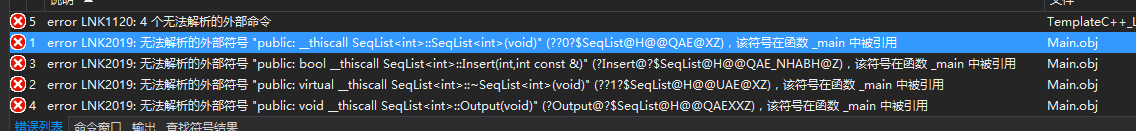
\includegraphics[width = 14cm]{MustKnowError.png}
			\caption{Error: 没包含cpp文件}
		\end{figure}
		
	\textbf{解决方法}:同时包含.cpp与.h文件,或将实现写入.h文件
		\begin{figure}[h]
			\centering
			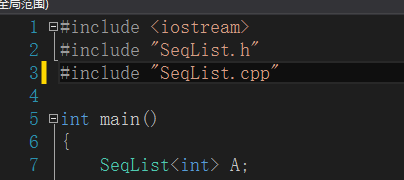
\includegraphics[scale = 0.6]{TemplateFirst.png}
			\caption{解决LNK2019 问题}
		\end{figure}	
 
 
	 \paragraph{特点}
		 \begin{itemize}
			 \item 抽象性:模版代码高度抽象,是函数和类的模范
			 \item \textbf{安全性}:型式检查能够发现大多数型式失配问题
			 \item \textbf{通用性}:函数和类模版定义一次,按需生成函数和类的实体
			 \item 易用性:接口相对直观且高度一致
			 \item \textbf{效率}: 减少冗余代码,提高编程效率,通过编译优化,提升程序执行效率
		 \end{itemize}
	
	\paragraph{用途}
		\begin{itemize}
			\item \textbf{函数模板}:构造函数集,实现不依赖特定数据结构的抽象算法
			\item \textbf{类模板}:构造类集,实现抽象数据结构
			\item \textbf{元编程}:构造在编译期执行的运算,提升程序执行效率
		\end{itemize}	 
		
\section{函数模版}
	\subsection{定义及使用}
			\begin{lstlisting}
	template <typedname AnyType>
	void Swap(AnyType &a, AnyType &b)
	{
		AnyType  temp;
		temp = a;
		a = b;
		b = temp;
	}			
			\end{lstlisting}
			
	\subsection{声明模版函数}
		\begin{lstlisting}			
	template<typename T>
	void Swap(T &a, T &b);			
		\end{lstlisting}
			
	\subsection{模版也可以重载}
			
	\subsection{实参的演绎-模版类型推导确定}
				
				当我们调用某些模版时,模板参数可以由我们所传递的实参来决定。如下
			\begin{lstlisting}
	template <typename T>
	inline T const& max(T const& a, T const& b);
			
	max(4,7);		//Ok: 两个实参的类型都是int
	max(4,4.2);		//ERROR: 第一个T为int,第二个T为double
			\end{lstlisting}
			
			有三种方法可以处理上面的错误:
			\begin{enumerate}[itemindent = 1em]
				\item 对实参进行强制类型转换,使他们可以相互匹配: max(static\_cast<double>(4),4.2);
				\item 显示指定T的类型:max<double>(4,4.2); 
				\item 指定两个参数可以具有不同的类型
			\end{enumerate}
			
	\subsection{定制非模版函数(重载函数模版)}
			函数模板功能非常强大,但是有时候可能会陷入困境,加入待比较的函数模板没有提供正确的操作符,或者提供的操作对某些特定的类型会产生不正确的操作结果,则程序不会对此进行编译。为了避免这种错误,可以使用函数模板和同名的非模板函数重载,这就是\textbf{函数定制},以完成对特定的类型等完成特定的功能.
			
			函数模板与同名的非模板函数重载必须遵守以下规定:
			\begin{itemize}[itemindent = 1em]
				\item 寻找一个参数完全匹配的\textbf{函数},如有,则调用它
				\item 如果失败,寻找一个\textbf{函数模板},使其实例化,产生一个匹配的模板函数,若有,则调用它
				\item 如果失败,再试低一级的对函数重载的方法,例如通过类型转换可产生的参数匹配等,若找到匹配的函数,调用它
			\end{itemize}
		\begin{lstlisting}
	// 定义函数模板,找出三个值中最小的值,与数据类型无关 
	template <class T> 
	T min(T ii, T jj, T kk) 
	{ 
		T temp; 
		if((ii<jj)&&(ii<kk)){        temp=ii;    } 
		else if((jj<ii)&&(jj<kk)){        temp=jj;    } 
		else    {        temp=kk;    } 
		return temp; 
	} 
	//非模板函数重载 
	const char* min(const char* ch1, const char* ch2,const char* ch3) 
	{ 
		const char* temp; 
		int result1 = strcmp(ch1,ch2); 
		int result2 = strcmp(ch1,ch3); 
		int result3 = strcmp(ch2,ch1); 
		int result4 = strcmp(ch2,ch3); 
		if((result1<0)&&(result2<0))    {        temp = ch1;    } 
		else if((result3<0)&&(result4<0))    {        temp=ch2;    } 
		else    {        temp=ch3;    } 
		return temp; 
	} 
	void main() 
	{ 
		cout<<min(100,20,30)<<endl; 
		cout<<min(10.60,10.64,53.21)<<endl; 
		cout<<min('c','a','C')<<endl;     
		cout<<min("anderson","Washington","Smith")<<endl; //正常输出 Smith
	} 	
		\end{lstlisting}
\section{函子}
	编写函数,求某个数据集的最小元,元素型式为T
	
	实现策略:使用\textbf{函数指针}作为回调函数参数
	
	实现策略:使用\textbf{函子(function object,functor)}作为回调函数参数
	
	\subsection{函数指针实现}
		\begin{lstlisting}
	template< typename T >
	const T & Min( const T * a, int n, bool (*comparer)(const T&, const T&) )
	{
		  int index = 0;
		  for( int i = 1; i < n; i++)
		  {
			    if( comparer( a[i], a[index] ) )
				      index = i;
		  }
		  return a[index];
	}
	
		\end{lstlisting}
	
	\subsection{函子}
		\subparagraph{目的}:
			\begin{itemize}
				\item 功能上:类似函数指针
				
				\item 实现上:重载函数调用操作符,必要时重载小于比较操作符
			\end{itemize}
			
		\subparagraph{优点}:
			\begin{itemize}
				\item 函数指针不能内联,而函子可以,效率更高
				
				\item 函子可以拥有任意数量的额外数据,可以保存结果和状态,提高代码灵活性
				
				\item 编译时可对函子进行型式检查
			\end{itemize}
			
		\subparagraph{例子}\verb|->|
		
			\begin{lstlisting}
	template< typename T >  class Comparer
	{
	public:
		  //  确保型式T已存在或重载operator<
		  bool operator()( const T & a, const T & b )  {  return a < b;  }
	};
	
	template< typename T, typename Comparer >
	const T & Min( const T * a, int n, Comparer comparer )
	{
		  int index = 0;
		  for( int i = 1; i < n; i++)
		  {
			    if( comparer( a[i], a[index] ) )    index = i;
		  }
		  return a[index];
	}
	
	
	//  使用方法
	int a[8] = { 9, 2, 3, 4, 5, 6, 7, 8 };
	int min = Min( a, 8, Comparer<int>() );    //  构造匿名函子作为函数参数
			\end{lstlisting}		
			
\section{类模板}
		\subsection{定义类模板}
			\begin{lstlisting}	
	//.h file		
	template <Class Type>    //First imoprtant thing
		
	class Stack
	{
	private:
		enum {MAX = 10};     //constant specific to class
		Type items[MAX];
		int  top;
	public:
		Stack();
		bool isEmpty();
		bool push(const Type& item);
		bool pop(Type &item);
	};		    
			\end{lstlisting}
				
				
		\subsection{使用类模板}
			\begin{lstlisting}	
	//.cpp file		
	template <class Type>
	bool Stack<Type>::isEmpty()
	{
		return top==0;
	}			
			\end{lstlisting}
			
		\subsection{类模板别名}
			\begin{lstlisting}			
	typedef std::array<double,12> arrd;
		
	arrd gallons;			
			\end{lstlisting}
	
	
		\subsection{类模板显示特化}
			使用特定的型或值显式特化类模板,\textbf{以定制类模板代码}
			
			\begin{lstlisting}
	template<> class A<char> { … };
			\end{lstlisting}

			\begin{itemize}
				\item 显式特化版本\textbf{覆盖}体化版本
				
				\item 显式特化并\textbf{不要求}与原始模板\textbf{相同},特化版本可以具有不同的数据成员或成员函数
				
				\item 类模板可以部分特化,结果仍是类模板,以支持类模板的部分定制
			\end{itemize}
\section{模版参数}
	\subsection{非类型模版参数}
		\verb|template<class T, size_t N> class Stack{};|
	\begin{lstlisting}
	template<class T, size_t N> class Stack{
		T data[N]; // Fixed capacity is N
		size_t count;
		
	public:
		void push(const T& t);
	};
	
	template<class T>
	inline void Stack<T>::push(const T& t){// Something}
	\end{lstlisting}

	\subsection{默认模版参数}
		\verb|template<class T, size_t N = 100> class Stack{};|
	
		\begin{lstlisting}
	template<class T = int, size_t N = 100>
	class Stack{
		T data[N];
		size_t count;
	public:
		void push(const T& t);
	};
	
	Stack<> myStack; 	// Same as Stack<int, 100>
		\end{lstlisting}
	
	\subsection{模版类型的模版参数}
	\verb|template<class T, template<class U> class Seq> class Container{};|
	
	\begin{lstlisting}
	template<class T, template<class U> class Seq>
	class Container{
		Seq<T> seq;
	public:
		void append(const T& t){seq.push_back(t);}
		// Other Stuffs
	};
	
	Container<int, vector> container;
	\end{lstlisting}
	
	\subsection{typename}
	 必须 对 \textbf{模版中的嵌套 类型}使用 \verb|typename|进行说明,否则模版会编译不过
	\begin{lstlisting}
	template<class T, template<class U, class = allocate<U> > class Seq>
	void printSeq(const Seq<T>& seq)
	{
		for(typename Seq<T>::iterator b = seq.begin(); b != seq.end();)
		{
			cout<< *b++ <<endl;
		}
	}
	\end{lstlisting}
	
	\subsection{模板类中再有模版成员}
		\begin{lstlisting}
	template<typename T> class complex{
		template<class X> complex(const complex<X>&);
	};
	
	complex<float> z(1,2);
	complex<double> w(z);
	
	int data[5] = {1, 2, 3, 4, 5};
	vector<int> v1(data, data+5);
	vector<double> v2(v1.begin(),v1.end());
		\end{lstlisting}



\section{模版特化}
	\paragraph{特化}将类型抽取出来固定,那么前面就不再具有泛化类型,\verb|template<被抽取走>  class specialLize<用特化的类型放到此处>|,可以理解为模版针对不同参数的重载。
	
	\subsection{全特化 Full Specialization}
		\verb|template<>|
		\begin{lstlisting}
// 函数特化
	template<class T> const T& min(const T& a, const T& b)
	{
		return (a<b) ? a:b;
	}
	
	// An explicit sepcialization of the min template
	template<>
	const char* const& min<const char*> (const char* const& a, const char* const& b)
	{
		return (strcmp(a,b) < 0) ? a : b;
	}
	
// 类特化
	template<class T, class Allocator = allocator<T> > class vector{};
	// 全特化	
	template<> class vector<bool, allocator<bool> >{};	
		\end{lstlisting}
	\subsection{偏特化 Partial Specialization}
		改变多模版参数的一个为固定值,或同类型的指针类型,然后特化函数
		\begin{lstlisting}
	// 偏特化  第一个参数特化,第二参数不特化
	template<class Alloc> class vector<bool, Alloc> {};
		\end{lstlisting}
\section{模版友元}
	\begin{lstlisting}
	// Necessary forward Declarations;
	template<class T> class Frinedly;
	template<class T> void f(const Friendly<T> &);
	
	template<class T> class Friendly
	{
		T t;
	public:
		Friendly(const T& theT):t (theT){}
		// f后的<> 必不可少,要不就是普通函数而不是模版函数了
		friend void f<>(const Friendly<T>&);
		void g(){ f(*this); }
	}
	
	
	// 特化 友元
	
	template<class T> class Friendly
	{
		template<class U> friend void f<>(const Friendly<U>&);
		/*
			由于友元声明的模版参数独立于T,因此任意的T和U的组合都允许使用,形成友元关系
			
			像成员模版一样,友元模版也可以出现 在 非模版类中。
		*/
	}
	\end{lstlisting}	
	
\section{元编程}
	

\section{enable\_shared\_from\_this}
	
	
\section{参考}\url{http://developer.51cto.com/art/201208/351569.htm}    

\chapter{Effective}
	\section{Effective C++}
		\subsection{C++ 基本相关性能提升}
		\paragraph{1.尽量以const,enum,inline替换\#define} 编译过程:\verb|.c|文件--预处理-->\verb|.i|文件--编译-->\verb|.o|文件--链接-->\verb|bin|文件
		
		多了类型检查,因为\verb|#define| 只是单纯的替换
		\paragraph{2.尽可能使用const} const允许你告诉编译器和其他程序员某值应保持不变,\textbf{只要“某值”确实是不该被改变的,那就该确实说出来}。
		\paragraph{3.确定对象被使用前已先被初始化}
			\subparagraph{赋值与初始化} C++规定,对象的成员变量的初始化动作发生在进入构造函数本体之前。所以应将成员变量的初始化置于构造函数的初始化列表中
			
			\begin{lstlisting}
ABEntry::ABEntry(const std::string& name, const std::string& address,
const std::list<PhoneNumber>& phones)
{ 
	theName = name;                //这些都是赋值,而非初始化
	theAddress = address;          //这些成员变量在进入函数体之前已调用默认构造函数,接着又调用赋值函数,
	thePhones = phones;            //即要经过两次的函数调用。            
	numTimesConsulted = 0;
} 
	 
ABEntry::ABEntry(const std::string& name, const std::string& address,
const std::list<PhoneNumber>& phones) 
:theName(name),                    //这些才是初始化 
 theAddress(address),                //这些成员变量只用相应的值进行拷贝构造函数,所以通常效率更高。
 thePhones(phones),
 numTimesConsulted(0){} 
			\end{lstlisting}
				
			\subparagraph{Note}  C++有着十分固定的“成员初始化次序”。\textbf{基类总是在派生类之前被初始化},而\textbf{类的成员变量总是以其说明次序被初始化}。所以:\verb|当在成员初始化列表中列各成员时,最好总是以其声明次序为次序|。
		\subsection{C++ 构造/析构/赋值性能提升}
		\paragraph{4.C++默认编写并调用哪些函数} 如果你\textbf{自己没声明},\textbf{编译器就会}为类声明(编译器版本的)一个\textbf{拷贝构造}函数,一个\textbf{拷贝赋值操作符}和一个\textbf{析构}函数。此外\textbf{如果你没有声明任何构造函数},\textbf{编译器也会}成为你声明一个默认构造函数。所有这些函数都是\verb|public|且\verb|inline|,编译器产生规则如下:

			\begin{itemize}
				\item \verb|调用准则|:\textbf{惟有}当这些函数\textbf{被需要}(被调用),它们才会被编译器创建出来。即有需求,编译器才会创建它们。
				\item \verb|析构函数|:\textbf{编译器产生的析构函数}是个\verb|non-virtual|,\textbf{除非}这个类的\textbf{基类自身声明有}\verb|virtual|析构函数
				\item \verb|拷贝构造|:至于\textbf{拷贝构造函数和拷贝赋值操作符},编译器创建的版本\textbf{只是单纯地}\textit{将}来源对象的\textbf{每一个非静态成员变量}\textit{拷贝到}目标对象 (\verb|浅拷贝|)
				\item \verb|构造函数|:如一个类\textbf{声明了一个构造函数}(无论有没参数),编译器\textbf{就不再为}它创建默认构造函数
			\end{itemize}
				
		\paragraph{5.若不想使用编译器自动生成的函数,就该明确拒绝} 为驳回编译器自动(暗自)提供的机能,可将相应的成员函数声明为\verb|private|并且不予实现。使用像\verb|noncopyable|这样的基类也是一种做法, 除此C++11 提供\verb|=delete| 关键字可以完成该操作。
			
		\paragraph{6.为多态基类声明virtual析构函数} 当基类的指针指向派生类的对象的时候,当我们使用完,对其调用\verb|delete|的时候,其结果将是未有定义——基类成分通常会被销毁,而派生类的充分可能还留在堆里。这可是形成资源泄漏、败坏之数据结构、在调试器上消费许多时间
			
			消除以上问题的做法很简单:给基类一个\verb|virtual|析构函数。此后删除派生类对象就会如你想要的那般。
			
			 \verb|STL容器|都不带\verb|virtual|析构函数,所以最好别派生它们
			 
		\begin{lstlisting}[frame = lbrT,xleftmargin=.02\textwidth]
// Note:
1、带有多态性质的基类应该声明一个virtual析构函数。如果一个类带有任何virtual函数,它就应该拥有一个virtual析构函数

2、一个类的设计目的不是作为基类使用,或不是为了具备多态性,就不该声明virtual析构函数
		\end{lstlisting}
				 
		\paragraph{7.别让异常逃离析构函数} 析构函数绝对不要吐出异常。如果一个被析构函数调用的函数可能抛出异常,析构函数应该捕捉任何异常,然后吞下它们(不传播)或结束程序
		
		\paragraph{8.决不让构造和析构过程中调用virtual函数} 基类的构造函数的执行要早于派生类的构造函数,当基类的构造函数执行时,派生类的成员变量尚未初始化。派生类的成员变量没初始化,即为指向虚函数表的指针\verb|vptr|没被初始化又怎么去调用派生类的\verb|virtual|函数呢?析构函数也相同,派生类先于基类被析构,又如何去找派生类相应的虚函数?
		
		\paragraph{9.令operator= 返回一个reference to *this}
			对于赋值操作符,我们常常\textbf{要达到}这种类似效果,即\textbf{连续赋值}
			\begin{lstlisting}[xleftmargin=.04\textwidth]
 int x, y, z;
 x = y = z = 15;
 
 赋值采用右结合律,所以上述连锁赋值被解析为
 x = (y = (z = 15));
 这里15先被赋值给z,然后其结果(更新后的z) 再赋值给y,然后其结果(更新后的y)再赋值给x.
			\end{lstlisting}
			
			为了实现“连锁赋值”,赋值操作符必须\textbf{返回一个“引用”}指向操作符的左侧实参,这个协议适合所有的赋值运算。
			\begin{lstlisting}[xleftmargin=.04\textwidth]
Widget&  operator = (const Widget &rhs)
{
	...
	return *this;
}

class Widget{
public:
	Widget& operator+=(const Widget& rhs)   //这个协议使用于所有赋值相关运算 (+=, -=, *=等)
	{
		...
		return *this;
	}
	
	Widget& operator= (int rhs)
	{
		...
		return *this;
	}
};
			\end{lstlisting}
		\paragraph{10.在operator =中处理“自我赋值”}
			自我赋值如下所示:
		\begin{lstlisting}
Widget w;
w = w;
a[i] = a[j]; //i == j or i != j
*px = *py;	 // px,py指向同个地址;
		\end{lstlisting}
		
		\begin{lstlisting}
// 该怎么做
Widget& Widget::operator=(const Widget& rhs)
{ 
	Widget temp(rhs);
	swap(temp);
	return *this;
} 
		\end{lstlisting}
		
		“许多时候一群精心安排的语句就可以导出异常安全(\verb|new| 新对象时出错,那么原来的东西亦将不复存在)(自我赋值)的代码。”以下note给出正确做此事的规矩.
		\begin{lstlisting}[frame = lbrT]
1、确保当对象自我赋值时operator =有良好行为。其中技术包括比较“来源对象”和“目标对象”的地址、精心周到的语句顺序、以及copy-and-swap
2、确定任何函数如果操作一个以上的对象,而其中多个对象是同一个对象时,其行为仍然正确
		\end{lstlisting}	
				
		\paragraph{11.复制对象时勿忘其每一个成员} 如果你为class \textbf{添加一个成员变量},你必须同时修改 复制构造函数 和 赋值操作符函数,当\textbf{使用继承时},子类需重写 拷贝构造,且\textbf{不要忘了基类的成分}
		
			\begin{lstlisting}
PriorityCustomer::PriorityCustomer(const PriorityCustomer& rhs)
: 	Customer(rhs), 			// 调用 Base类的拷贝构造函数
	priority(rhs.priority)
{
	logCall("PriorityCustomer Copy constructor");
}

PriorityCustomer& operator=(const PriorityCustomer& rhs)
{
	Customer::operator=(rhs);  	// 对Base  类成分进行赋值动作
	priority = rhs.priority;
	return (*this);
}
			\end{lstlisting}
		

	\subsection{资源管理}
		\paragraph{12.以对象管理资源} 使用\verb|shared_ptr| 等代理对象管理指针
		\paragraph{13.在资源管理类中小心拷贝行为}
		\paragraph{14.在资源管理类中提供对原始资源的访问}
		\paragraph{15.成对使用new和delete时要采取相同形式}
		\paragraph{16.以独立语句将newed对象置入智能指针}
	\subsection{设计与声明}
		\paragraph{17.让接口容易被正确使用,不易被误用}
		\paragraph{18.设计class犹如设计type}
		\paragraph{19.宁以pass-by-reference-to-const替代psss-by-value} 这种传递方式效率高得多:没有任何构造函数或析构函数被调用,因为没有任何新对象被创建。
		
		\paragraph{20.必须返回对象时,别妄想返回其reference}
			函数创建新对象的途径有二:在栈空间和堆空间
			
			\begin{itemize}
				\item \textbf{栈上}:即在函数内的局部变量。局部变量在函数返回后就没有存在的意义,若还对它“念念不忘”,将带来灾难性后果。所以传引用在栈上不可行
				\item \textbf{堆上}:在堆上构造一个对象,并返回。看似可行,也埋下了资源泄漏的危险。谁该对这对象实施delete呢?别把这种对资源的管理寄托完全寄托于用户。所以传引用在堆上不可行
				\item \textbf{静态对象}:出于我们对多线程安全性的疑虑,以及当线程中两个函数对单份对象的处理也可能带来不可测行为。所以静态对象也是不可行的
			\end{itemize}
			
			一个“必须返回新对象”的函数的正确写法是:就让那个函数返回一个新对象
		\paragraph{21.将成员变量声明为private}
		\paragraph{22.宁以non-member、non-friend替换member函数} 这样做可以增加封装性、包裹弹性和\textbf{机能扩充性}
		\paragraph{23.若所有参数皆需类型转换,请为此采用non-member函数}
		\paragraph{24.考虑写出一个不抛异常的swap函数}
	\subsection{实现}
		\paragraph{25.尽可能延后变量定义式的出现时间}
		\paragraph{26.尽量少做转型动作}
		\paragraph{27.避免返回handls指向对象内部成分}
		\paragraph{28.为“异常安全”而努力是值得的}
		\paragraph{29.透彻了解inlining的里里外外}
		\paragraph{30.将文件间的编译依存关系降至最低}
	\subsection{继承与面向对象设计}
		\paragraph{31.确定你的public继承塑模出is-a关系}
		\paragraph{32.避免遮掩继承而来的名称}
		\paragraph{33.区分接口继承和实现继承}
			\verb|public|继承分为:1、\verb|接口继承|2、\verb|实现继承|
			\begin{itemize}
				\item 成员函数的接口总是会被继承
				\item 声明一个\textbf{纯虚函数}的目的是为了\textbf{让派生类继承函数接口}-\verb|"变化性"|
				\item 声明一个\textbf{虚函数}的目的是\textbf{让派生类继承该函数的接口和缺省实现}-\verb|"不变性,与变化性"|
				\item 声明一个\textbf{非虚函数}的目的是\textbf{为了令派生类继承函数的接口及一份强制性实现}-\verb|"不变性,凌驾特异性"|
			\end{itemize}
		\paragraph{34.考虑virtual函数以外的其它选择}
		\paragraph{35.绝不重新定义继承而来的non-virtual函数}
		\paragraph{36.绝不重新定义继承而来的缺省参数值}
		\paragraph{37.通过符合塑模出has-a或“根据某物实现出”}
	\section{More Effective C++}
		\subsection{基础议题(Basics)}
			\paragraph{1.仔细区别 pointers 和 references}
				在任何情况下都\textbf{不能使用}\textit{指向空值}的\textbf{引用}。一个引用必须总是指向某些对象。在C++里,引用应被初始化,不存在指向空值的引用这个事实意味着使用引用的代码效率比使用指针的要高。因为在使用引用之前不需要测试它的合法性。
				
				指针与引用的另一个重要的不同是指针可以被重新赋值以指向另一个不同的对象。但是引用则总是指向在初始化时被指定的对象,以后不能改变
				
				总的来说,在以下情况下你应该\textbf{使用指针},\textit{一是}你考虑到存在不指向任何对象的可能(在这种情况下,你能够设置指针为空),\textit{二是}你需要能够在不同的时刻指向不同的对象(在这种情况下,你能改变指针的指向)。如果总是指向一个对象并且一旦指向一个对象后就\textit{不会改变指向},那么你应该\textbf{使用引用}。
				还有一种情况,就是当你\textbf{重载某个操作符}时,你应该使用引用
			\paragraph{2.最好使用 C++ 转型操作符}
				\verb|static_cast<double>(value)|
				
			\paragraph{3.绝对不要以多态方式处理数组} 继承 后仍然使用 基类数组,导致数组的下标运算出现问题,因为数组是根据元素的sizeof 进行计算下一个元素出现的位置,如果派生类的 sizeof 值不同,将会出现内存错误。
				\begin{lstlisting}
	#include <iostream>
	using namespace std;
	
	struct B
	{
		virtual void print() const{cout<<"base print()"<<endl;}
	};
	struct D : B
	{
		void print() const{cout<<"derived print()"<<endl;}
		int id;  //如果没有此句,执行将正确,因为基类对象和子类对象长度相同  
	};
	
	int fun(const B array[],int size)
	{
		for(int i = 0;i<size;++i)
		{
			array[i].print();
		}
	}
	
	int main()
	{
		B barray[5];
		fun(barray,5);
		D darray[5];
		fun(darray,5);
	}
				\end{lstlisting}
			\paragraph{4.避免无用的 default constructors}
			
		\subsection{操作符(Operators)}
			\paragraph{5.对定制的“类型转换函数”保持警觉}
				\textbf{定义类似功能的函数},而抛弃隐式类型转换,\textbf{使得类型转换必须显示调用}。例如 \verb|String|类没有定义对\verb|Char*|的隐式转换,而是用\verb|c_str|函数来实施这个转换。拥有单个参数(或除第一个参数外都有默认值的多参数)构造函数的类,很容易被隐式类型转换,最好加上 \verb|explicit| 防止\textbf{隐式类型转换}
				
				\subparagraph{隐身类 类型抓换}
					\begin{itemize}
						\item  可以用 \textbf{单个形参来调用} 的构造函数定义了\textit{从} \textbf{形参类型 到 该类类型} 的一个隐式转换,这里应该注意的是, “可以用单个形参进行调用” 并不是指构造函数只能有一个形参,而是它可以有多个形参,但那些形参都是有默认实参的。
						\begin{lstlisting}
	#include <string>
	#include <iostream>
	using namespace std ;
	class BOOK  //定义了一个书类
	{
	private:
		string _bookISBN ;  //书的ISBN号
		float _price ;    //书的价格
	
	public:
		//定义了一个成员函数,这个函数即是那个“期待一个实参为类类型的函数”
		//这个函数用于比较两本书的ISBN号是否相同
		bool isSameISBN(const BOOK & other ){
			return other._bookISBN==_bookISBN;
		}
	
		//类的构造函数,即那个“能够用一个参数进行调用的构造函数”(虽然它有两个形参,但其中一个有默认实参,只用一个参数也能进行调用)
		BOOK(string ISBN,float price=0.0f):_bookISBN(ISBN),_price(price){}
	};
	
	int main()
	{
		BOOK A("A-A-A");
		BOOK B("B-B-B");
		
		cout<<A.isSameISBN(B)<<endl;   //正经地进行比较,无需发生转换
		
		cout<<A.isSameISBN(string("A-A-A"))<<endl; //此处即发生一个隐式转换:string类型-->BOOK类型,借助BOOK的构造函数进行转换,以满足isSameISBN函数的参数期待。
		cout<<A.isSameISBN(BOOK("A-A-A"))<<endl;    //显式创建临时对象,也即是编译器干的事情。
		
		system("pause");
	}
						\end{lstlisting}
						
							代码中可以看到,\verb|isSameISBN|函数是期待一个\verb|BOOK|类类型形参的,但我们却传递了一个\verb|string|类型的给它,这不是它想要的啊!还好,\verb|BOOK|类中有个构造函数,它使用一个\verb|string|类型实参进行调用,编译器调用了这个构造函数,隐式地将\verb|stirng|类型转换为\verb|BOOK|类型(构造了一个BOOK\textbf{临时对象}),再传递给\verb|isSameISBN|函数。
							
							隐式类类型转换还是会带来风险的,正如上面标记,\textbf{隐式转换得到类的临时变量,完成操作后就消失了},我们构造了一个完成测试后被丢弃的对象。
						\item 隐式类型转换运算符只是一个样子奇怪的成员函数:\verb|operator| \textbf{关键字},其后跟一个类型符号。你不用定义函数的返回类型,因为返回类型就是这个函数的名字。例如\textbf{为了允许}\verb|Rational|(有理数)类\textbf{隐式地转换为}\verb|double|类型(在用有理数进行混合类型运算时,可能有用),你\textbf{可以如此声明}\verb|Rational|类
						
						\begin{lstlisting}
	class Rational {
	public:
		...
		operator double() const; // 转换Rational类成 double类型
	}; 
	
	Rational r(1, 2); // r 的值是1/2
	double d = 0.5 * r; // 隐式转换 r 到double,
						\end{lstlisting}
					\end{itemize}
				
				\subparagraph{避免 隐身转换}	一般来说,越有经验的C++程序员就越喜欢避开类型转换运算符。例如在\verb|C++|标准库委员会工作的人员是在此领域最有经验的,他们加在库函数中的\verb|string|类型没有包括隐式地从\verb|string|转换成C风格的\verb|char*|的功能,而是定义了一个成员函数\verb|c_str|用来完成这个转换,这是巧合么?我看不是。
					\begin{itemize}
						\item 声明装换功能的函数,如\verb|string| 的\verb|c_str()|函数
						\item \verb|explicit operator Type() const;|
						\item \verb|explicit BOOK(string ISBN,float price=0.0f);|
					\end{itemize}
					
			\paragraph{6.区别 increment/decrement 操作符的前置和后置形式}
			\paragraph{7.千万不要重载 \&\&, || 和 , 操作符}
			\paragraph{8.了解各种不同意义的 new 和 delete}
				\subparagraph{new操作符(new operator)和new操作(operator new)的区别}
					当你写这样的代码:
					\verb|string *ps = new string("Memory Management");|
					你使用的\verb|new是new操作符|。这个操作符就象\verb|sizeof|一样是语言内置的,你不能改变它的含义,它的功能总是一样的。它要完成的功能分成两部分。\textbf{第一部分}是分配足够的内存以便容纳所需类型的对象。\textbf{第二部分}是它调用构造函数初始化内存中的对象。new操作符总是做这两件事情,你不能以任何方式改变它的行为。
					
					你所能改变的是如何为对象分配内存。\verb|new|操作符调用一个函数来完成必需的内存分配,你能够重写或重载这个函数来改变它的行为。\verb|new|操作符为分配内存所调用函数的名字是\verb|operator new|。
					函数\verb|operator new| 通常这样声明:
					\verb|void * operator new(size_t size);|
					
					就象\verb|malloc|一样,\verb|operator new|的职责\textbf{只是分配内存}。它对构造函数一无所知。
			
				\subparagraph{placement new}
		\subsection{异常(Exceptions)}
			\paragraph{--堆栈辗转开解stack-unwinding}如果一个函数中出现异常,在函数内即通过 \verb|try..catch| 捕捉的话,可以继续往下执行;如果不捕捉就会抛出(或通过 \verb|throw |显式抛出)到外层函数,则当前函数会终止运行,释放当前函数内的局部对象(局部对象的析构函数就自然被调用了),外层函数如果也没有捕捉到的话,会再次抛出到更外层的函数,该外层函数也会退出,释放其局部对象……如此一直循环下去,直到找到匹配的 catch 子句,如果找到 main 函数中仍找不到,则退出程序。
			
			\paragraph{9.利用 destructors 避免泄漏资源}
			\paragraph{10.在 constructors 内阻止资源泄漏} 使用智能指针 在初始化列表中进行初始化 堆上资源可以防止 异常情况下的资源泄漏,\textbf{其实,防止内存泄漏就用 智能指针的手段就可以了}
			
			\paragraph{11.禁止异常流出 destructors 之外}
				这一条讲得其实是捕获析构函数里的异常的重要性。第一是防止程序调用 \verb|terminate| 终止(这里有个名词叫:堆栈辗转开解 \verb|stack-unwinding|);第二是析构函数内如果发生异常,则异常后面的代码将不执行,无法确保我们完成我们想做的清理工作。
				
				之前我们知道,析构函数被调用,会发生在对象被删除时,如栈对象超出作用域或堆对象被显式 \verb|delete| (还有继承体系中,virtual 基类析构函数会在子类对象析构时调用)。除此之外,在异常传递的堆栈辗转开解(\verb|stack-unwinding|)过程中,异常处理系统也会删除局部对象,从而调用局部对象的析构函数,而此时如果该析构函数也抛出异常,C++程序是无法同时处理两个异常的,就会调用 \verb|terminate()|终止程序(会立即终止,连局部对象也不释放)。另外,如果异常被抛出,析构函数可能未执行完毕,导致一些清理工作不能完成。
				
				所以不建议在析构函数中抛出异常,如果异常不可避免,则应在析构函数内捕获,而不应当抛出
				
			\paragraph{12.了解 "抛出一个 exception ”  与 “传递一个参数” 或 “调用一个虚函数”之间的差异}
			\paragraph{13.以 by reference 方式捕捉 exceptions} 提高效率
			
			\paragraph{14.明智运用 exception specifications} 毫无疑问,异常规格是一个引人注目的特性。它使得代码更容易理解,因为它明确地描述了一个函数可以抛出什么样的异常
			\paragraph{15.了解异常处理的成本}
			
		\subsection{效率(Efficiency)}
			\paragraph{16.谨记 80-20 法则}
			\paragraph{17.考虑使用 lazy evaluation(缓式评估)}
			\paragraph{18.分期摊还预期的计算成本}
			\paragraph{19.了解临时对象的来源}
			\paragraph{20.协助完成“返回值优化(RVO)}
			\paragraph{21.利用重载技术避免隐式类型转换}
			\paragraph{22.考虑以操作符复合形式(op=)取代其独身形式(op)}
			\paragraph{23.考虑使用其它程序库}
			\paragraph{24.了解 virtual functions、multiple inheritance、virtual base classes、runtime type identification 的成本 }
			
		\subsection{技术(Techniques,Idioms,Patterns)}
			\paragraph{25.将 constructor 和 non-member functions 虚化}
			\paragraph{26.限制某个 class 所能产生的对象数量}
			\paragraph{27.要求(或禁止)对象产生于 heap 中}
			\paragraph{28.Smart Pointer(智能指针)}
			\paragraph{29.Reference counting(引用计数)}
			\paragraph{30.Proxy classes(替身类、代理类)}
			
		\subsection{杂项讨论(Miscellany)}
			\paragraph{31.在未来时态下发展程序}
			\paragraph{32.将非尾端类设计为抽象类}	
				
	\section{Effective Modern C++}
		\subsection{Deducing Types}
		\subsection{auto}
		\subsection{Moving to Modern C++}
		\subsection{Smart Pointers}
		\subsection{Rvalue References, Move Semantics, and Perfect Forwarding}
		\subsection{Lambda Expressions}
		\subsection{The Concurrency API}
		\subsection{Tweaks}
	\section{Effective STL}
		\subsection{容器}
			\paragraph{1.慎重选择容器类型,根据需要选择高效的容器类型}
			\paragraph{2.不要试图编写独立于容器类型的代码}
			\paragraph{3.确定容器中的对象拷贝正确而高效。也就是防止在存在继承关系时发生剥离}
			\paragraph{4.调用empty而不是检查size()是否为0来判断容器是否为空} 原因是调用\verb|empty|比检查size()更加高效
			\paragraph{5.尽量使用区间成员,而不是多次使用与之对应的单元素成员函数,原因是这样更加高效} 如尽量使用\verb|vector|的\verb|assign|或\verb|insert|成员函数,而不是一直使用\verb|push_back|
			\paragraph{6.小心C++编译器最烦人的分析机制}
			\paragraph{7.如果在容器中包含了能过new操作创建的指针,切记在容器对象析构前将指针delete掉} 使用智能指针如\verb|shared_ptr|(C++11)是个比较好的选择
			\paragraph{\sout{8.切勿创建包含auto\_ptr的容器对象}} \verb|auto_ptr|不是采用引用计数实现的,放进容器中就等着出问题吧,特别是当对容器使用\verb|sort|这类会对元素进行赋值的算法之后
			
			\paragraph{9.慎重选择删除元素的方法} 这一点很重要,因为在删除一个元素之后会导致一些迭代器、指针及引用失效。所以如果手写循环删除元素一定要小心。最好的方法是\verb|vector、string、deque|采用\verb|erase-remove|这样的习惯写法,方便又安全,\verb|list|应当使用成员函数\verb|remove|,\textbf{关联容器}使用成员函数\verb|erase|。
				
			要小心的一点是算法\verb|remove|并不是真正的删除容器中的元素,因为它没有这个能力,它只能将无用的元素移去末尾。之后你必须用成员函数\verb|erase|删除无用区间
			\paragraph{10.了解分配器allocator的约定和限制}
			\paragraph{11.理解自定义分配器合理用法}
			\paragraph{12.切勿对STL容器的线程安全性有不切实际的依赖} 请手工保证线程安全,不要依赖\verb|STL|
		\subsection{vector And string}
			\paragraph{13.尽量用vector和string代替动态分配的数组}
			\paragraph{14.使用reserve来避免不必要的内存重新分配} 成员函数\verb|reserve|可以为容器预留一块内存,当容器大小(size)增大时,\textbf{不用重新分配内在,可以提高效率}。需要缩减分配的内存时可以使用后面提到的\verb|swap技术|,或者使用成员函数\verb|.shrink_to_fit|
			
			\paragraph{15.注意string实现的多样性}
			\paragraph{16.了解如何把vector和string数据传给旧的C API} \verb|vector|请使用 \verb|&vector[0]|,当然先要确定容器不为空。\verb|string|使用\verb|c_str()|方法
			
			\paragraph{17.使用“swap 技巧”除去多余的容量} 与临时变量交换,然后利用 临时变量的 RAII 机制,保证了在任何情况下,使用对象时先构造对象,最后析构对象。从而在析构该临时对象时 将空间释放掉
			
			\paragraph{18.避免使用vector<bool>} 因为它不是容器,它是用位来存储\verb|bool|值的,所以它也没有迭代器,不能对其使用标准算法。最好使用\verb|deque <bool> 或bitset|代替之
			
		\subsection{关联容器}
			\paragraph{19.理解相等equality 和等价equivalence 的区别} 在实际中相等的概念是基于 \verb|operator==| 的。\verb|find|对“相同”的定义是相等,是以 \verb|operator==|为基础的; \verb|set::instert|对“相同”的定义是等价,是以\verb|operator< |为基础的
			
			\paragraph{20.为包含指针的关联容器指定比较类型}	默认情况的比较类型是 \verb|less<T>|,所以\textbf{只会比较指针的值},\textit{而不是}\textbf{指针指向的值},所以需要手工指定比较类型,以比较指针指向的值。
			
			\paragraph{21.总是让比较函数在等值情况下返回false} 特别是在关联容器基于比较函数判断等价的情况下。否则会导致相同的值按照定义是不等价的
			\paragraph{22.切勿直接修改set 或 multiset中的键} 会破坏该数据结构。而\verb|map|中的键被\verb|const|修饰,不能更改
			\paragraph{23.考虑用排序的vector 替代 关联容器}
			\paragraph{24.当效率至关重要时,请在map::operator[]与map::insert之间做出谨慎选择} 选择的标准是:当向\verb|map|中添加元素时,要优先选择\verb|insert|; 当更新已经在\verb|map|中的元素的值时,要优先选择\verb|operator[]|
			\paragraph{25.熟悉散列容器} \verb|unordered_map、unordered_multimap、unordered_set、unordered_multiset|
		\subsection{迭代器}
			\paragraph{26.尽量使用iterator,而不是const\_iterator、reverse\_iterator及const\_reverse\_iterator} 使用\verb|iterator|会减少很多麻烦,所以使用STL时尽量使用\verb|iterator|
			
			\paragraph{27.使用distance和advance将容器的const\_iterator转换成iterator} 首先明确的是不能使用\verb|const_cast|进行转换,因为这两个根本就是两个完全不相关的类,比\verb|string和complex<double>|之间的关系还远。可以使用下面的技术转换,\verb|i是iterator|类型,\verb|ci是const_iterator|类型:
			
				\begin{lstlisting}
typedef IntDeque::const_iterator ConstIter;
advance(i, distance<ConstIter>(i, ci));   // <ConstIter> 不能少,否则编译通不过
				\end{lstlisting}
			\paragraph{28.正确理解由reverse\_iterator的base()成员函数所产生的iterator的用法} 向右有一个位置的偏移,保证了对于插入操作而言,\verb|ri和ri.base()|是等价的
			
			对于删除而言则不是等价的,要先\verb|++ri|,如\verb|v.erase((++ri).base())|;	
			\paragraph{29.对非格式化的逐个字符的输入考虑使用 istreambuf\_iterator} 比\verb|istream_iterator|效率更高而且更方便(不用清\verb|iOS::skipws|标志)。相对的还有\verb|ostreambuf_iterator|
		\subsection{算法}
			\paragraph{30.确保目标区间足够大}:
			
			\verb|transform(values.begin(), values.end(), results.end(), transmogrify); |
			
			可以更改为
			
			\verb|transform(values.begin(), values.end(), back_inserter(results), transmogrify);|
			
			应该使用插入迭代器。插入迭代器有 \verb|inserter|、\verb|back_inserter|、\verb|front_inserter|、\verb|ostream_iterator|
			\paragraph{31.了解各种与排序有关的选择}
				\subparagraph{非稳定排序}都要求随机访问迭代器 \verb|RandomAccessIterator| 
					\begin{itemize}[itemindent = 1em]
						\item \verb|sort|:基于快排的排序
						\item \verb|partial_sort|:部分排序,指定排序区间
						\item \verb|nth_element|:将排序后位于前n个位置的元素放在前n个位置,但不对它们进行排序。
					\end{itemize}
				\subparagraph{稳定排序}
				
					\begin{itemize}[itemindent = 1em]
						\item \verb|stable_sort|:稳定排序,排序后等价元素的相对位置不会变
						\item \verb|list::sort|
					\end{itemize}
				\subparagraph{分割序列的算法}
					只需要双向迭代器
					\begin{itemize}[itemindent = 1em]
						\item \verb|partition|
						\item \verb|stable_partition|:不改变相同元素顺序
					\end{itemize}
			\paragraph{32.如果确实需要删除元素,则需要在remove这一类算法之后调用成员函数erase}
				算法\verb|remove|\textbf{不能真正删除元素},因为它没有这个能力,\textbf{必须调用}类似\verb|erase|这样的成员函数才行,\verb|list|的成员\verb|remove|\textbf{可以真正删除元素}。类似\verb|remove|这样的算法有\verb|remove_if、unique|
				
			\paragraph{33.对包含指针的容器使用remove这一类算法时要特别小心} 因为被“删除“的值可能也不存在于序列最后面,而是被覆盖了。与\verb|remove|算法的实现有关
			
			\paragraph{\sout{34.了解哪些算法要求使用排序区间作为参数}}
			\paragraph{\sout{35.通过mismatch或lexicographical\_compare实现简单忽略大小写的字符串比较}}
			
			\paragraph{36.理解copy\_if算法的正确实现}
			\paragraph{37. 使用accumulate或者for\_each进行区间统计}
		\subsection{函数子、函数子类、函数及其他}
			\paragraph{38.遵循按值传递的原则来设计函数子类} 在STL中,函数对象往往会按值传递和返回,所以在设计函数对象时要保证经过了值传递之后还能正常工作
			
			\paragraph{39.确保判别式predicate是纯函数pure function} "\verb|纯函数|"是指返回值仅仅依赖于其参数的函数
			\paragraph{40.若一个类是函数子,则就使它可配接adaptable}
			\paragraph{41.理解ptr\_fun、mem\_fun、mem\_fun\_ref的来由}
			\paragraph{42.确保 less<T>与operator< 具有相同的语义}
		\subsection{在程序中使用STL}
			\paragraph{43.算法调用优先于手写的循环}
			\paragraph{44.容器的成员函数优于同名的算法} 因为成员函数更高效,成员函数可以根据特定的容器及实现作出优化
			\paragraph{45.正确区分 count、find、binary\_search、lower\_bound、upper\_bound 和 equal\_range} 根据需要选择最高效的算法
				
				\begin{figure}[h]
					\centering
					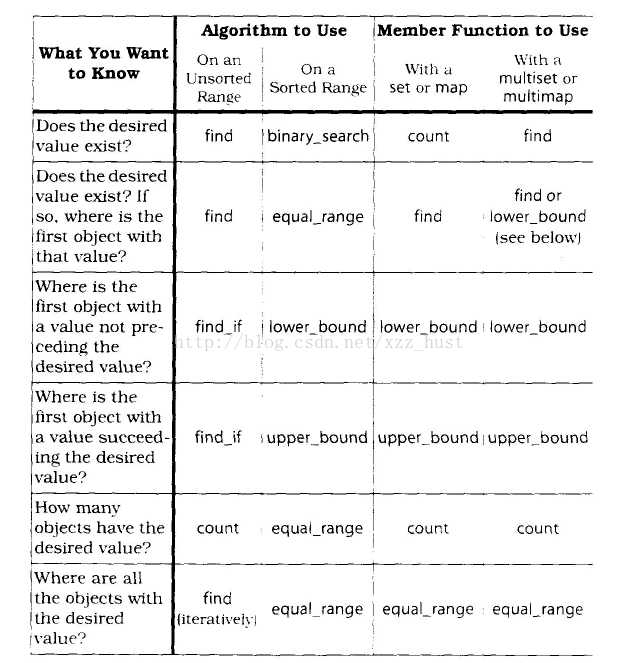
\includegraphics[scale = 0.7]{STL-Effective.png}
				\end{figure}
			\paragraph{46.考虑使用函数对象而不是函数作为STL算法参数} 一个事实是STL的sort比C语言标准中的qsort更快。原因就是sort使用函数对象,而qsort使用函数指针作为参数。\textbf{如果一个函数对象的}\verb|operator()|\textbf{已经被声明为内联的},那么其在函数体内也是内联的,但对于函数指针就不一样了,通过函数指针传递的函数不大可能会被优化成内联的,即使该函数被声明为内联的。
			
			\paragraph{47.避免产生“直写型(write-only)”代码} "直写型"代码复杂而难以理解,不便于维护。”直写型“代码就是那种一句话完成n多功能的代码,晦涩难懂。最好将”直写型“代码分解为易读的代码
			
			\paragraph{48.总是包含(\#include)正确的头文件}
			\paragraph{49.学会分析与STL相关的编译器诊断信息}

	\section{提升C++编程性能的技术}
		\subsection{跟踪范例}
			\subparagraph{关注点} 本章引入的实际问题为:定义一个简单的Trace类,将当前函数名输出到日志文件中。Trace对象会带来一定的开销,因此\textit{在默认情况}下\textbf{不会开启Trace功能}。
			
			问题是:\verb|怎么设计Trace类,使得在不开启Trace功能时引入的开销最小|
			
			\subparagraph{解决方案} 
				\begin{enumerate}
					\item \textbf{宏}:用\textbf{宏}来\verb|开关Trace功能|很简单,在不开启时开销完全没有
					\begin{lstlisting}
#ifdef TRACE
Trace trace("aaa");
#endif
					\end{lstlisting}
						
					\item \textbf{静态状态变量}:使用状态变量的话有一定的运行时开销,但能保证灵活性,是一种比较合理的选择
					\begin{lstlisting}
class Trace {
public:
	...
	static bool isTraceEnabled;
	void Debug() {
		if (isTraceEnabled) {
			...
		}
	}
}
					\end{lstlisting}
				\end{enumerate}
				
			\subparagraph{涉及技术- 延迟创建} 原本的\verb|Trace|类中内置\verb|string|成员,这样在不开启\verb|Trace|时也要承担构造和析构的开销。可以将其改为\verb|string*|,并在真正需要开启时再创建该成员。
			
			如果\verb|Trace|的开启时间远小于总时间,则此方法很有效,否则当动态创建的开销大于固定的1次构造和析构的开销时,原方法更好一些
			
		\subsection{虚函数}
		\subsection{临时对象}
			\subparagraph{关注点} 如何避免产生不必要的临时对象
			
			\subparagraph{类型不匹配} 在\textbf{不同类型间}的\textbf{赋值}容易无意中导致临时对象的创建。可以通过在单参数构造函数前加\verb|explicit|来避免这种隐式的转换产生
			
			\subparagraph{避免重复创建相同的临时对象} 临时对象有一个就够了..相同的对象的反复创建无形的增加了 工作量
				\begin{lstlisting}
Complex a;
for (int i = 0; i < 10; ++i) {
	a += 1.0;
}

其中每次循环都会创建一个值为1.0的Complex对象。可以在循环外创建一个值为1.0的Complex对象,来减少这种开销:
Complex one(1.0);
for (int i = 0; i < 10; ++i) {
	a += one;
}
				\end{lstlisting}
		\subsection{内存池}
			\subsubsection{单线程内存池}
				\subparagraph{关注点} 默认的通用内存管理器的性能在特定场景下会造成一定的性能瓶颈。本章讨论的是在单线程环境下,每次分配固定大小和不固定大小的内存时,实现比通用\verb|new/delete|性能更好的内存池管理器
				
				\subparagraph{Rational 专用内存池} 每次分配\verb|Rational|大小的内存块,用一个空闲链表维护已分配的空闲内存,在释放时重新将此内存块放回到链表中
				
				\begin{lstlisting}
class Rational {
	...
	static list<char *> freeList;
	void *operator new(size_t size) {
		if (freeList.empty()) {
			return new char[sizeof(Rational)];
		} else {
			void *buf = freeList.back();
			freeList.pop_back();
			return buf;
		}
	}
	void operator delete(void *ptr, size_t size) {
		freeList.push_back(ptr);
	}
};
				\end{lstlisting}
				
				\textbf{此版本的内存池}从不收缩,如果需要释放内存,则需要新增一个接口。
				
				\textbf{此版本的内存池}与通用内存管理器相比,收益在于:
					\begin{itemize}[itemindent = 1em]
						\item 每次分配的大小为固定值,不用在空闲列表中进行大量的查找(直接返回末端指针)。
						\item 不用处理并发情况,没有临界区						
					\end{itemize}
				
				\subparagraph{固定大小内存池实现} 不只针对Rational,而是扩展为支持任意固定大小的类:
					\begin{lstlisting}
template <typename T>
class FixedSizeMemoryPool {
public:
	FixedSizeMemoryPool(): size_(sizeof(T))
	{}
	~FixedSizeMemoryPool() {
		for(char *&p: freeList_) {
			delete[] p;
		}
	}
	void *Alloc() {
		if (freeList_.empty()) {
			return new char[size_];
		} else {
			void *buf = freeList_.back();
			freeList_.pop_back();
			return buf;
		}
	}
	void Free(void *buf) {
		freeList_.push_back(buf);
	}
private:
	list<char *> freeList_;
	const size_t size_;
};

// Rational则需要改为:
class Rational {
public:
	void *operator new(size_t size) {
		return pool.Alloc();
	}
	void operator delete(void *ptr, size_t size) {
		pool.Free(ptr);
	}
private:
	static FixedSizeMemoryPool<Rational> pool;
};
					\end{lstlisting}
				\subparagraph{不定大小内存池} 不定大小的内存池的管理方法与上面的版本不同,因为没有办法直接从链表中返回一个内存块(大小不同)。这里我们在需要时分配一个大的固定大小的内存块,每次分配单个对象的内存时就从这个内存块上分配,空间不够时就分配大的内存块。
				
				随着通用性的增加,性能也在逐渐下降。因此,在非常需要性能时,牺牲一些灵活性通用性也许会有很好的效果。
			\subsubsection{多线程内存池} 在Alloc和Free时加锁,其它保持不变

		\subsection{引用计数}
			\subparagraph{关注点} \verb|C++|使用了引用计数\textbf{来解决垃圾回收问题},基本思想是\textbf{把对象清除的责任}\textit{从}客户端代码\textbf{转移给}对象本身。
			
			引用计数可以\textbf{减少内存使用}、\textbf{避免内存泄漏},但在执行速度方面却可能会有坏处,尤其是在多线程环境中
			
			\subparagraph{引用计数的实现}方案1:
			\begin{lstlisting}
class RefCountBase {
public:
	Attach() {
		++refCount_;
	}
	Detach() {
		if (--refCount_ == 0) {
			delete this;
		}
	}
protected:
	RefCountBase(): refCount_(0) {}
	RefCountBase(const RefCountBase &rc): refCount_(0) {}
	RefCountBase &operator=(const RefCountBase &rc) {
		return *this;
	}
	virtual ~RefCountBase() {}
	
	size_t refCount_;
};

如类A继承自RefCountBase,为了实现引用计数,还需要一个代理类SmartPtr充当A的智能指针
template <typename T>
class SmartPtr {
public:
	SmartPtr(T *ptr = nullptr): ptr_(ptr) {}
	SmartPtr(const SmartPtr &sptr): ptr_(sptr.ptr_) {
		if (ptr_) {
			ptr_->Attach();
		}
	}
	SmartPtr &operator=(const SmartPtr &sptr) {
		if (sptr.ptr_) {
			sptr.ptr_->Attach();
		}
		if (ptr_)
		ptr_->Detach();
		
		ptr_ = sptr.ptr_;
		return *this;
	}
	T *operator->() { return ptr_; }
	T &operator*() ( return *ptr_; )
private:
	T *ptr_;
};
			\end{lstlisting}
			
			实现B:将计数功能放入\verb|SmartPtr|中。去掉\verb|RefCountBase|,而是在\verb|SmartPtr|中增加 一个\verb|size_t| \verb|*count_|,对\verb|ptr_的Attach|操作变为\verb|++*count_|,而\verb|Detach|操作则变为\verb|--*count_|。其它相同
			
			\subparagraph{并发引用计数} \verb|SmartPtr|中需要同时对\verb|count_和ptr_|进行操作,在并发环境下这就意味着\textbf{需要在操作前后加锁},来\textbf{保证}对两个对象的\textbf{原子操作},从而避免数据竞争
			
			\subparagraph{引用计数的性能} 实现\verb|A|中需要对原类进行修改,如果不能进行这种修改,则只能使用实现\verb|B|。实现\verb|B|中因为需要操作\textbf{两个堆上的成员}(\verb|count_和ptr_|),创建和清除性能会比实现\verb|A|差一些
			
			\textbf{优点}:
				\begin{lstlisting}[frame = lbrT]
1、 防止内存泄露
2、 高效的赋值操作。尤其是作为写时复制(COW)的重要环节,如果赋值后很少有修改操作的话,相比于深复制,引用计数的收益非常明显
3、 节省内存空间。尤其是体积非常大的对象
4、 可以方便的实现RAII。将引用计数的Detach操作变为某种关闭操作,则可很方便地实现RAII
				\end{lstlisting}
			
			\textbf{缺点}:
				\begin{lstlisting}[frame = lbrT]
1、 COW中如果修改较多,那么性能相比深复制不一定有提升
2、 在并发环境下对它的操作还有锁的开销,可能会影响性能比较多
				\end{lstlisting}
			
			下列条件会\textbf{增加引用计数的收益}:
				\begin{lstlisting}[frame = lbrT]
1、 目标对象消耗大量资源
2、 资源的分配和释放很昂贵
3、 目标对象高度共享
4、 引用的创建和清除很廉价
				\end{lstlisting}
		\subsection{循环引用}
			参考文献:\url{http://www.cnblogs.com/TianFang/archive/2008/09/20/1294590.html}
		
			引用计数是一种便利的内存管理机制,但它有一个很大的缺点,那就是不能管理循环引用的对象。一个简单的例子如下:
			\begin{lstlisting}
	#include <string>
	#include <iostream>
	#include <boost/shared_ptr.hpp>
	#include <boost/weak_ptr.hpp>
	
	class parent;
	class children;
	
	typedef boost::shared_ptr<parent> parent_ptr;
	typedef boost::shared_ptr<children> children_ptr;
	
	class parent
	{
		public:
		~parent() { std::cout <<"destroying parent\n"; }
		
		public:
		children_ptr children;
	};
	
	class children
	{
		public:
		~children() { std::cout <<"destroying children\n"; }
		
		public:
		parent_ptr parent;
	};
	
	
	void test()
	{
		parent_ptr father(new parent());
		children_ptr son(new children);
		
		father->children = son;
		son->parent = father;
	}
	
	void main()
	{
		std::cout<<"begin test...\n";
		test();
		std::cout<<"end test.\n";
	}	
			\end{lstlisting}
		运行该程序可以看到,即使退出了\verb|test|函数后,由于\verb|parent和children|对象互相引用,\textbf{它们的引用计数都是1,不能自动释放},\textit{并且此时这两个对象再无法访问到}。\textbf{这就引起了c++中那臭名昭著的内存泄漏}。	
			
		一般来讲,解除这种循环引用有下面有三种可行的方法:
			\begin{enumerate}[itemindent = 1em]
				\item 当只剩下最后一个引用的时候需要手动打破循环引用释放对象。
				\item 当parent的生存期超过children的生存期的时候,children改为使用一个普通指针指向parent。
				\item 使用弱引用的智能指针打破这种循环引用。
			\end{enumerate}
		虽然这三种方法都可行,但方法1和方法2都需要程序员手动控制,麻烦且容易出错。这里主要介绍一下第三种方法和boost中的弱引用的智能指针\verb|boost::weak_ptr|。
		
			\subparagraph{强引用弱引用}
				一个强引用当被引用的对象活着的话,这个引用也存在(就是说,\textbf{当至少有一个强引用,那么这个对象就不能被释放})。\verb|boost::share_ptr|就是强引用。
				
				相对而言,弱引用当引用的对象活着的时候不一定存在。仅仅是当它存在的时候的一个引用。弱引用并不修改该对象的引用计数,这意味这弱引用它并不对对象的内存进行管理,\textbf{在功能上类似于普通指针},然而一个比较大的区别是,\textbf{弱引用能检测到所管理的对象是否已经被释放},从而避免访问非法内存。	
				
			
			\subparagraph{通过弱引用打破循环引用}
				由于弱引用不更改引用计数,类似普通指针,只要把循环引用的一方使用弱引用,即可解除循环引用。对于上面的那个例子来说,只要把children的定义改为如下方式,即可解除循环引用:
				\begin{lstlisting}
	class children
	{
	public:
		~children() { std::cout <<"destroying children\n"; }
	
	public:
		boost::weak_ptr<parent> parent;
	};
				\end{lstlisting}
			
			最后值得一提的是,虽然通过弱引用指针可以有效的解除循环引用,但这种方式必须在程序员能预见会出现循环引用的情况下才能使用,也可以是说这个仅仅是一种编译期的解决方案,如果程序在运行过程中出现了循环引用,还是会造成内存泄漏的。因此,不要认为只要使用了智能指针便能杜绝内存泄漏。毕竟,对于C++来说,由于没有垃圾回收机制,内存泄漏对每一个程序员来说都是一个非常头痛的问题。
		
			\subparagraph{实践操作示例}
				参考文献:\url{https://blog.csdn.net/xtzmm1215/article/details/45868835}
				\begin{lstlisting}
	class B;  
	class A  
	{  
		public:// 为了省去一些步骤这里 数据成员也声明为public  
		weak_ptr<B> pb;  
		//shared_ptr<B> pb;  
		void doSomthing()  
		{  
			shared_ptr<B> pp = pb.lock();  
			if(pp)//通过lock()方法来判断它所管理的资源是否被释放  
			{  
				cout<<"sb use count:"<<pp.use_count()<<endl;  
			}  
		}  
		
		~A()  
		{  
			cout << "kill A\n";  
		}  
	};  
	
	class B  
	{  
		public:  
		//weak_ptr<A> pa;  
		shared_ptr<A> pa;  
		~B()  
		{  
			cout <<"kill B\n";  
		}  
	};  
	
	int main(int argc, char** argv)  
	{  
		shared_ptr<A> sa(new A());  
		shared_ptr<B> sb(new B());  
		if(sa && sb)  
		{  
			sa->pb=sb;  
			sb->pa=sa;  
		}  
		sa->doSomthing();  
		cout<<"sb use count:"<<sb.use_count()<<endl;  
		return 0;  
	}  
				\end{lstlisting}
				
		\subsection{代码优化}
		\subsection{设计优化}
		\subsection{可伸缩性}
		\subsection{系统体系结构相关性}

	\section{深入探索 C++ 对象模型}
	
	\section{STL 源码剖析}
	
	\section{参考}
		\paragraph{Effective C++} \url{http://blog.csdn.net/shenzi/article/details/5601038}
		
		\paragraph{More Effective C++} \url{http://www.cnblogs.com/tianyajuanke/archive/2012/11/29/2795131.html}
		
		\paragraph{Effective Mordern C++} \url{http://blog.csdn.net/cteng/article/details/41912179}
		
		\paragraph{Effective STL} \url{http://blog.csdn.net/xzz_hust/article/details/9624613}
		
		\paragraph{提高C++性能的编程技术} \url{http://www.cnblogs.com/fuzhe1989/p/3546598.html}
		
		\paragraph{STL 源码剖析} \url{http://blog.csdn.net/shenya1314/article/details/54923558}
%%%%%%%%%%%%%%%%%%%%%%%%%%%%%%%%%%%%%%%%%%%%%%%%%%%%%%%%%%%%%%%%%%%%%%%CHAPTER_并行库_OpenMP_Using%%%%%%%%%%%%%%%%%%%%%%%%%%%%%%%%%
\chapter{OpenMP 并行技术}


\chapter{GPU 并行技术}
	\section{OpenCL}
	
	\section{CUDA}

\end{document} 
 		    